\documentclass[usetitle=true, journal=jpclcd, manuscript=letter]{achemso}

\usepackage[version=4]{mhchem}
\usepackage{color}
\usepackage{geometry}
\geometry{letterpaper}                     % ... or a4paper or a5paper or ... 
%\geometry{landscape}                		   % Activate for for rotated page geometry
%\usepackage[parfill]{parskip}    		     % Activate to begin paragraphs with an empty line rather than an indent
\usepackage{graphicx}
\usepackage{subcaption}				
\usepackage{amssymb}
\usepackage{amsmath}
\usepackage{setspace}
\usepackage[T1]{fontenc}
\usepackage{siunitx} %BRJ added. is this OK??
\usepackage{chemmacros}

\usepackage{xspace}

\DeclareSIUnit{\molar}{M}
\DeclareSIUnit[number-unit-product = {\,}]
\cal{cal}
\DeclareSIUnit\kcal{\kilo\cal}


\newcommand{\kon}{$k_{\textrm{on}}$\xspace}
\newcommand{\koff}{$k_{\textrm{off}}$\xspace}
\let\oldAA\AA
\renewcommand{\AA}{\oldAA\xspace}
\newcommand{\bcd}{$\beta$-cyclodextrin\xspace}


\title{Quantitative Ranking of Ligand Binding Kinetics 
		with a Multiscale Milestoning Simulation Approach}

% author list
\author{Benjamin R. Jagger} 
\affiliation[Dept. of Chemistry and Biochemistry, University of California, San Diego]
{Department of Chemistry and Biochemistry, University of California, San Diego, 
9500 Gilman Drive, La Jolla, California 92093-0340, United States}

\author{Christopher T. Lee} 
\affiliation[Dept. of Chemistry and Biochemistry, University of California, San Diego]
{Department of Chemistry and Biochemistry, University of California, San Diego, 
9500 Gilman Drive, La Jolla, California 92093-0340, United States}

\author{Rommie E. Amaro} 
\affiliation[Dept. of Chemistry and Biochemistry, University of California, San Diego]
{Department of Chemistry and Biochemistry, University of California, San Diego, 
9500 Gilman Drive, La Jolla, California 92093-0340, United States}
\email{ramaro@ucsd.edu}

\begin{document}

\newpage

\begin{abstract}
\section{abstract}
Predicting the rate of nonfacilitated permeation of solutes across lipid bilayers is important to drug design, toxicology, and signaling. These rates can be estimated using molecular dynamics simulations combined with the inhomogeneous solubility-diffusion model, which requires calculation of the potential of mean force and position-dependent diffusivity of the solute along the transmembrane axis. In this paper, we assess the efficiency and accuracy of several methods for the calculation of the permeability of a model DMPC bilayer to urea, benzoic acid, and codeine. We compare umbrella sampling, replica exchange umbrella sampling, adaptive biasing forces, and multiple-walker adaptive biasing forces for the calculation of the transmembrane PMF. No definitive advantage for any of these methods in their ability to predict the permeability coefficient \perm~was found, provided that a sufficiently long equilibration is performed. For diffusivities, a Bayesian inference method was compared to a Generalized Langevin method, both being sensitive to chosen parameters and the slow relaxation of membrane defects.
%{\bf Although the performance for predicting log Pm was generally fair, the accuracy of these calculations could be improved by the development of more accurate force fields and methods for the calculation of the PMF and diffusion coefficient profiles.}
Agreement within 1.5 log units of the computed \perm~with experiment is found for all permeants and methods.  Remaining discrepancies can likely be attributed to limitations of the force field as well as slowly relaxing collective movements within the lipid environment.  Numerical calculations based on model profiles show that \perm~can be reliably estimated from only a few data points, leading to recommendations for calculating \perm~from simulations.

% suggestion from Chris C.:
%Although the agreement with experiment, however perfectible, is by and large reasonable, the present set of calculations brings to light aspects where improvement is desirable. While the methodology is robust and has proven appropriate for a variety of applications, sampling remains a major concern, in particular for the estimation of diffusivities, owing to the slowly relaxing collective movements within the lipid environment. The discrepancies between theory and experiment also illustrate the shortcomings of macromolecular force fields in describing small, drug-like permeants.

%YW: replacing the last sentence with something on concentrating the computing resources on a few data points? sth like: Our analysis also shows that only a few data points on the PMF and diffusivity profiles contribute significantly to Pm. For this reason, we recommend focusing computational resources on these critical points, rather than evenly spreading them over the entire transmembrane axis.

\begin{tocentry}
\begin{center}
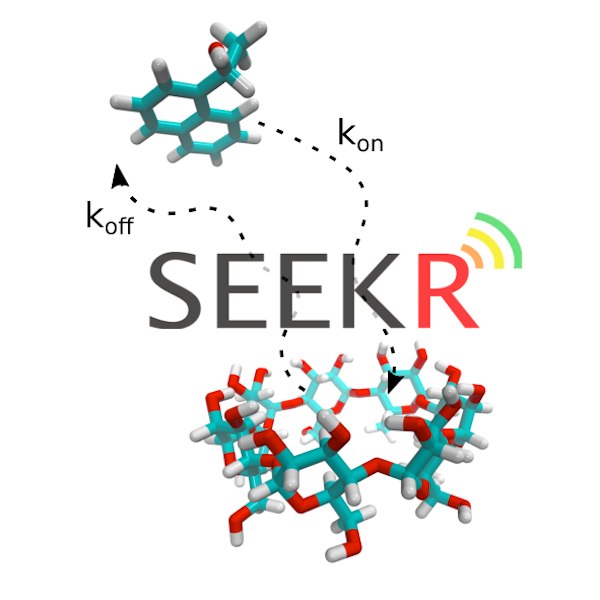
\includegraphics{images/bcd_toc.png}
\end{center}
\end{tocentry}
\end{abstract}

\newpage

%!TEX ROOT = ../ctl-phd-thesis.tex

\par The goal of biology is to understand life to an extent that one can predict the eventual behaviors of a living system under or in the absence of a stimulus or perturbation.
Although many debate the utility of quantitative modeling in answering this question, I will abstain from such discussion and focus on the benefits of modeling as I view them.
The development of a whole cell or organism model has become a hot topic in modern biology\cite{Roberts2014}.
As biologists uncover the mysteries which make life possible, they unveil new complexities\cite{CheckHayden2010}.
These complex and non-linear behaviors are not amenable to scrutiny via traditional research methods which are driven by classical hypotheses (i.e., by varying one parameter at a time and observing and characterizing the results to form conclusions).
Simple experimental models, while elegant, test isolated model behaviors in simplified systems which are often not generalizable.
In order to derive a general conclusion, many expensive experiments must be run to explore the solution space at large potential cost.

\par One strategy to reduce the experimental cost burden is to shift towards inexpensive mathematical modeling.
Mathematical models in biology are increasing in popularity, and come in a wide variety of flavors\cite{Gunawardena2014}.
For example, there are information and data driven models as well as models based on the fundamentals of physical principles.
In this dissertation, I will focus on the development of methods in support of the latter.
By codifying our knowledge of the physical world into a model, we can gain many benefits.
First, physical models can serve as a glue to reconcile the results of individual experiments under isolated conditions.
Cleverly designed mathematical models are also amenable to computed solutions using numerical methods.
Combining knowledge and computation, inexpensive parameter sweeps that eliminate physical impossibilities and guide experimental efforts can serve to reduce the experimental cost of biology.

\par Physical models can also produce other benefits for science.
During the design and validation phase of model construction, when a physical model fails to reproduce experimental results, this is a litmus test for the limitations of our current understanding.
By studying the assumptions of the model and querying the differences between prediction and experiment, scientists can pinpoint possible knowledge gaps.
Once a physical model is sufficiently validated, due to the fundamental basis of transferable physical properties, the models can also be used to generate prospective predictions.
For example, in an inspiring study, Hodgkin and Huxley created a famous model describing the propagation of an action potential along a giant squid axon\cite{HUXLEY1952}.
Although the model was based on empirical fitting of electrophysiology data, many speculated upon the physical implications of the mathematics.
One term in particular, predicting the presence of four voltage-sensitive gates in the sodium ion channel, was later experimentally confirmed by crystallographic structure which resolved the tetrameric channel structure\cite{Sigg2014a}.

\par We live in an exciting time, where there is a convergence of emerging structural data, legacy experimental parameters, and computational power.
In order to understand life, we must embrace the complexity of biology.
The work described in this dissertation seeks to address several challenges which hinder the routine application of large systems biology models.
This includes the computational prediction of various biological rates such as diffusion, permeability, and binding/unbinding, strategies to develop models of individual protein dynamics, and the capacity to generate multiscale geometric models suitable for biological modeling.

\section{Overview of Chapter Contents}

\par To reiterate and highlight the opportune convergence of computing and biological data, \cref{chap:exascale} discusses the potential applications and gains afforded by future exascale supercomputers to biology.
This chapter provides some perspective on the role that computers can play to solve various biological problems.
We speculate upon not only the contributions of computation to basic science, but also upon the impact of computation and technology on translational fields such as personalized medicine.
In this chapter, we also address and frame some of the aforementioned challenges to future modeling efforts with solutions described in the subsequent chapters.

\par Owing to the complexity of biology, a complete systems model will require the definition of many rates.
Due to the basic nature of many of these measurements, the experimental work to measure these values may not be publishable and is therefore difficult to source.
Although robotics which automate assay development and screening are amenable to some tasks, the complexity of experimental setups for measuring kinetic properties can often hinder accurate and high-throughput measurement.
To augment the existing data and measurements, molecular simulations such as Molecular Dynamics (MD) can be employed to generate estimates\cite{Leach2001,Durrant2011a}.
MD effectively integrates the classical equations of motion for an atomistic system.
Given that the typical timescales of simulation are typically much shorter than the timescales of the process of interest, brute force MD simulations can rarely capture the dynamics of interest with sufficient statistics.
Instead, using strategies derived from statistical mechanics, many enhanced sampling strategies have been developed to facilitate the estimation of classically intractable properties\cite{Chipot2007,Tuckerman2010}.
In \cref{chap:permeability}, we compare the efficiency of four enhanced sampling strategies to compute drug passive membrane permeability.
We find that there are many orthogonal degrees of freedom which can hinder the convergence of these calculations and recommend some best practices for future work.

\par While studying membrane permeability, I had many stimulating discussions with my colleague Lane Votapka on the topic.
During our overlap in the group, Lane was working on the development of a software tool which facilitates the use of milestoning to compute various rates.
Milestoning is another enhanced sampling strategy where, instead of observing the full transition from start to finish of a process, we collect statistics of transitions along many small segments of the full pathway and stitch them together in postprocessing\cite{Faradjian2004,Majek2010,Vanden-Eijnden2008,Kirmizialtin2011,Votapka2015,Bello-Rivas2015,Votapka2017c}.
The application of milestoning theory to permeability calculations was not straightforward since the natural currency of milestoning is transition probabilities, while the expressions to compute permeability required potentials of mean force.
To solve this, Lane derived a new relation to compute permeability values using transition probabilities from milestoning which we validated using a toy model inspired by my prior work on permeability.
This research is described in \cref{chap:mileperm}.

\par After learning about the virtues of the milestoning method, the group started thinking about possible applications of milestoning to compute other rates of interest.
By chance, my colleague Ben Jagger and I met Professor Chia-en Chang at a local conference where she was presenting preliminary results describing brute-force MD calculations of host-guest binding kinetics and thermodynamics\cite{Tang2017}.
This dataset which contained several ligands, experimentally determined kinetics, and brute-force MD was the ideal system to benchmark the use of SEEKR\cite{Votapka2017c}.
Chia-en kindly shared the dataset with us and working with Ben, we predicted the binding kinetics of the system using milestoning.
The results of this work are described in \cref{chap:bcd} along with some best practices to monitor the convergence of computed rate estimates which we developed along the way.

\par Also of interest for biological simulations is the dynamics of protein movement.
Not only are the dynamics of proteins critical to their biological function, but protein dynamics also influence phenomena such as drug binding.
In \cref{chap:allostery}, we present a review of many different strategies to use computers to inform the rational design of allosteric drugs.
Previously I had worked with Robert Malmstrom on a paper describing the applications of Markov state models to model protein kinase A dynamics with and without cyclic AMP\cite{Malmstrom2015a}.
During this project, we started thinking about the use of MSMs to model perturbations to the conformational ensembles of protein targets by drugs and using the information to support drug discovery efforts.
Later working with Bryn Taylor, we investigated the impact of drug binding to GPCR CCR2.
The generation and description of our CCR2 MSMs is presented in \cref{chap:ccr2}.

\par Another important aspect of cell modeling is the generation of computable geometries to represent cellular scenes.
Meshes are commonly used in engineering fields as a general geometric representation.
The use of meshes is desirable since they are often also compatible with simulation methods such as finite elements.
However, the numerical behavior of algorithms is often limited by mesh conditioning.
To support the development of robust mesh generation codes for biological geometries, working with John Moody, we developed the Colored Abstract Simplicial Complex library which is described in \cref{chap:asc}.

\par In summary, the work in this dissertation explores the use of various modeling strategies to predict values of interest or to generate geometric meshes in support of future multiscale modeling efforts.



%%!TEX root = bcd_SI.tex

\section*{Methods}
\subsection*{System Preparation} 
\par GAFF\cite{Wang2004,Wang2006} forcefield parameters for the seven guest molecule
along with both GAFF and Q4MD-CD\cite{Cezard2011} parameterizations of $\beta$-cyclodextrin 
were obtained from Tang and Chang\cite{Tang2017}. For comparison we use identical structure and
parameterizations as those used in their study. These initial structures were 
used by the SEEKR software for preparation of the milestoning simulations. 
The preparation procedure was the same for each of the seven guest molecules and 
followed standard SEEKR protocols\cite{Votapka2017}. All systems were solvated 
with TIP3P waters\cite{Jorgensen1983a}.

\subsubsection*{Preparation of milestoning simulations with SEEKR} 
\par The bound state of the host-guest complex was defined as the center of mass (COM) 
of the \bcd. The guest molecule was considered to be bound when 
its COM was within 1.5~\AA of the bound state coordinates. From this bound state, 
spherical milestones were defined in increasing 1.5~\AA increments from 1.5~\AA to
13.5~\AA. Furthermore, spherical milestones of radius 7.5~\AA and less, were 
divided into two half-spheres to better capture the asymmetries between the two faces. 
When the ligand is less than 7.5~\AA away from the bound state, it is trapped on 
a particular face due to the size of the host molecule. For milestone distances 
greater than 7.5~\AA, the ligand was found to freely sample both faces, and therefore 
a single spherical milestone was sufficient for sampling host-guest interactions. 
In total, 14 unique milestones were defined. In practice, this was achieved via 
post-processing the simulations on each face to identify any trajectories that 
crossed from one face to the other, and modifying the transitions accordingly in 
the milestoning model. In addition, two simulations were conducted for the outermost 
milestones (one with the ligand initiated on each face), and these were then 
combined into a single milestone (with double the sampling) for milestones that 
were not restricted to a particular face.


\par The first 13 milestones correspond to the MD region, while the 14th and 
outermost milestone corresponds to the BD region. The standard SEEKR preparation 
protocol\cite{Votapka2017} was then used to generate the coordinate, parameter, 
and simulation files necessary for a milestoning calculation. For each of the MD 
milestones, a copy of the apo \bcd structure was generated and the guest 
molecule was then placed at the appropriate radius from the bound state coordinates. 
Any water molecules that clashed with the guest molecule were removed. The guest 
distribution for the BD milestone was constructed by first running a conventional 
BD simulation where trajectories terminated at the appropriate distance for the 
milestone surface (13.5~\AA).

\subsection*{Simulation}
\subsubsection*{MD Simulations}
\par A modified version of NAMD 2.12 was used for all MD simulations\cite{Phillips2005}.
For all 13 milestones in the MD region, the standard SEEKR procedure for 
minimization, equilibration and simulation was followed. First, 5000 steps of 
minimization were performed to allow for relaxation, particularly of solvent, 
around the newly placed guest molecule. Further relaxation of the solvent was 
achieved by a series of 2~ps heating simulations that gradually increased the 
temperature from 298~K to 350~K and then cooled back to 298~K. Host and guest atoms 
were constrained during these heating simulations to ensure that the guest 
remained on the appropriate milestone surface. To obtain the equilibrium 
distribution of the guest molecule on each milestone, 200 ns of constant 
volume simulation was performed. A $\SI{90}{kcal\cdot mol^{-1}\cdot\angstrom^{-2}}$ 
harmonic restraint was used to hold the COM of the guest molecule at the appropriate 
distance from the binding site. To minimize any bias of the arbitrary guest 
starting conformation, the first 40~ns of each simulation were discarded and 
therefore were not included as part of the equilibrium distribution. From these 
trajectories, position and velocity configurations were selected every 0.2~ns, 
resulting in a total of 800 configurations per milestone. To obtain the first
hitting point distribution (FHPD) of each milestone, 10 independent and 
unrestrained simulations were initiated from these equilibrium configurations. 
Each simulation was propagated backwards in time by reversing its velocity at 
constant energy and volume (a total of 8000 reversals for each milestone). 
Only trajectories that struck an adjacent milestone before recrossing the 
milestone on which they originated were included as part of the FHPD for that 
milestone. To obtain the transition probabilities and times necessary for the 
calculation of kinetic parameters, all members of the FHPD were brought back to 
their starting position and velocity and new unrestrained simulations were then 
initiated from each configuration. These simulations were propagated forward in 
time at constant energy and volume. Once a simulation crossed its starting 
milestone again, it was monitored for crossing of adjacent milestones. 
When an adjacent milestone was crossed, the simulation was stopped and the 
transition and incubation time were recorded. Although more of the equilibrium 
simulation trajectories could likely have been used without biasing the results 
based on the starting conformation, the 8000 reversal trajectories that resulted 
from the 160~ns used were more than sufficient to sample the transitions between 
the milestones, resulting in hundreds of observed transitions between each milestone. 
In total, 2.6~${\mu}s$ of equilibrium sampling (160~ns for 16 milestones) were 
used and approximately 570~ns of FHPD sampling for a total of 3.2~${\mu}s$ of 
simulation used in the milestoning model. The total cost per ligand (including 
simulation discarded for equilibration) was therefore $\sim$3.8 ${\mu}s$. 
 %This is roughly half of the simulation time needed by Tang and Chang.

\subsubsection*{BD Simulations}
\par All BD simulations were performed using the BrownDye software package\cite{Huber2010}. 
Electrostatic potentials of the host and guest molecules used as inputs for the 
BD simulation were calculated with APBS version 1.4\cite{Baker2001}. To match 
experimental conditions, APBS calculations and BD simulations were carried out 
with a solvent dielectric of 78, a solute dielectric of 2, and zero ionic concentration. 
An initial series of simulations were initiated from the b-surface, a sphere that 
encloses the entire host molecule and has sufficient radius for the guest molecule 
to be situated in bulk solvent such that forces between the host and guest are centrosymmetric. 
$10^6$ independent BD simulations were initiated from random points on the b-surface 
and and were propagated until the guest either contacted the outermost milestone 
(13.5~\AA) or escaped. Trajectories that successfully contacted the 13.5~\AA milestone 
were used as the FHPD for this milestone. Another series of $10^6$ BD simulations 
were initiated from the FHPD and propagated until contacting the second-outermost 
milestone (12.0~\AA) or escaping to the q-surface. This procedure is automated by 
SEEKR.

\subsection*{Milestoning Calculations}
\par Statistics from all milestones in the MD and BD regions were extracted 
using SEEKR and combined to construct a transition kernel as well as an incubation 
time vector. These are the two key quantities for the calculation of kinetic 
parameters in milestoning theory.\cite{Faradjian2004} As described previously, 
a post-simulation analysis was performed to account for ligand transitions 
between the two faces of the \bcd ring for milestones of radius 7.5~\AA 
or less. The analysis portion of SEEKR was then used to compute the desired 
kinetic quantities, \kon and \koff, as well as the free energy of binding $\Delta G_{bind}$.


%!TEX root = BCD.tex

%\section*{Results and Discussion}

%\subsection*{Determination of Kinetic and Thermodynamic Parameters}

%Simulation data and the resulting milestoning model were used to calculate 
%both \kon (figure \ref{fig:on_scatter}) and \koff (figure \ref{fig: off_scatter}).
%Values obtained from SEEKR with both GAFF\cite{Wang2004,Wang2006} and Q4MD\cite{Cezard2011} forcefields are compared to experimentally available values \cite{Fukahori2004,Fukahori2006,Nishikawa2002,Nishikawa2006,Rekharsky1998,Barros1998}
%as well as the calculated long timescale MD values from Tang et al\cite{Tang2017}.

%put actual values in table in SI?

%\subsubsection*{On Rates}

\par SEEKR calculations and the long timescale MD simulations struggle to 
reproduce both the values and rank ordering of the experimentally determined \kon's (Fig.~\ref{fig:on_scatter}).
\begin{figure}
	\begin{subfigure}{\linewidth}
	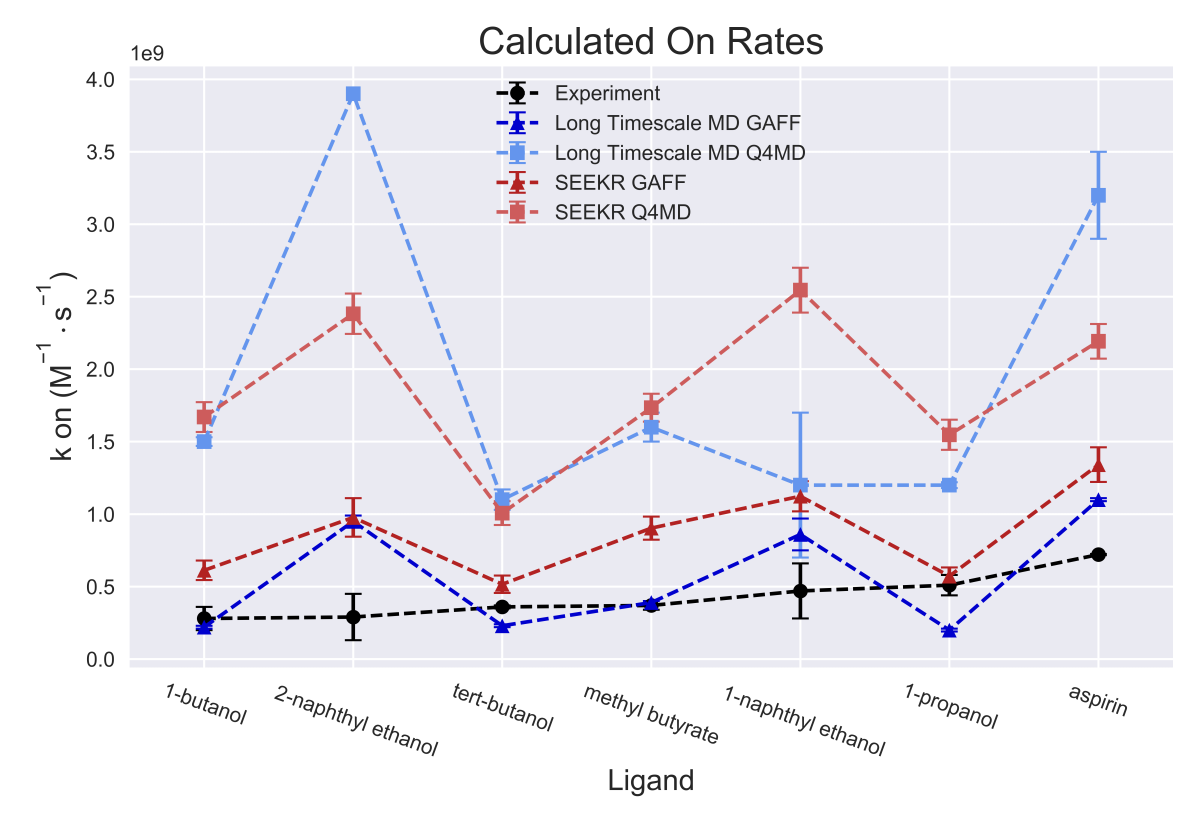
\includegraphics{images/on_scatter_resize.png}
	\caption{}
	\end{subfigure}

	\bigskip
	

	\begin{subfigure}{\linewidth}%<-- changed width
		%\centering
        %\renewcommand\tabularxcolumn[1]{m{#1}}% <-- added
        %\renewcommand\arraystretch{1.3}
        %\setlength\tabcolsep{2pt}% <-- added
    \begin{tabular}{
l  S[table-format = 2.3(3), separate-uncertainty] 
  S[table-format = 2.3(3), separate-uncertainty] 
 }%{\linewidth}%{*{4}{>{\centering\arraybackslash}X}}% <-- changed

\textbf{Method} & \textbf{Kendall} & \textbf{Spearman}  \\
\hline
      SEEKR GAFF      &    -0.20(31)           &    -0.29(40)            \\ 
      SEEKR Q4MD      &    0.14(29)           &    0.14(38)             \\ 
      Long Timescale MD GAFF      &    0.24(26)           &    0.25(29)                     \\ 
      Long Timescale MD Q4MD      &    0.00(28)           &    -0.05(37)                     \\ 
     

    \end{tabular}
        \caption{}
	\end{subfigure}
	\caption{a) Experimental and calculated on rates for SEEKR GAFF and Q4MD forcefields as well as long timescale MD with both forcefields. b) Calculated rank correlation coefficients. Errors are determined with a bootstrapping analysis. }
  \label{fig:on_scatter}
  \end{figure}
However, similar qualitative results are seen with the SEEKR calculations and 
long timescale MD calculations using the same forcefield.
%Chia-en directly from paper "GAFF-CD provided slightly more flexible β-CD, which produced more complicated H-bond
%networks between the free β-CD and water molecules in the first hydration shell, thereby resulting in slower kon and larger desolvation penalty"
On rates calculated using Q4MD are approximately one order of magnitude faster 
than experimental rates, while the GAFF forcefield produces rates closer to the 
experimental values, differing by approximately a factor of 3 or less.

\par Both methods fail to effectively order the ligands by increasing \kon, 
as demonstrated by low or negative Kendall and Spearman rank correlation coefficients.
As the values of all the experimental rates have limited variability (all within 
half an order of magnitude), the sensitivity of the methods as well as the errors 
associated with the calculations and experiments makes differentiation and 
ordering challenging. 
%Both simulation methods appear to show a stronger 
%dependence on the size and mass of the ligands than experiment, with both the 
%GAFF and Q4MD forcefields producing faster rates for larger compounds, a trend 
%not seen in the experimental rates.

%coment on uncharged small systems and how BD may struggle here?

 

%%!TEX root = BCD.tex

%%\documentclass[11pt,letterpaper]{article}

%%\usepackage{color}

%%\setlength{\textwidth}{17cm}
%%\setlength{\textheight}{20.5cm}
%%\setlength{\oddsidemargin}{-.1cm}
%%\setlength{\topmargin}{-2 cm}

%%\renewcommand{\baselinestretch}{1.0}

%%\newcommand{\hl}[1]{\textcolor{red}{#1}}
%\newcommand{\hl}[1]{\textbf{#1}}
%\providecommand{\e}[1]{\ensuremath{\times 10^{#1}}}

%%\begin{document}

\begin{table}

\centering
%\resizebox{\textwidth}{!}
{
\resizebox{\textwidth}{!}{\begin{tabular}{
l S[table-format = 2.3(3)e2, separate-uncertainty] |
l  S[table-format = 2.3(3)e2, separate-uncertainty] |
l S[table-format = 2.3(3)e2, separate-uncertainty]  |
l  S[table-format = 2.3(3)e2, separate-uncertainty] }

% \resizebox{\textwidth}{!}{\begin{tabular}{
% l S[table-format = 4.2(4)e8, separate-uncertainty, table-figures-uncertainty = 4.2] |
% l  S[table-format = 4.2e8, separate-uncertainty, table-figures-uncertainty = 4.2] |
% l S[table-format = 4.2e8, separate-uncertainty, table-figures-uncertainty = 4.2]  |
% l  S[table-format = 4.2e8, separate-uncertainty, table-figures-uncertainty = 4.2] |}

%\multicolumn{8}{c}{\kon rates}
\hline

 \multicolumn{2}{c}{\textbf{Experiment}} & \multicolumn{2}{c}{\textbf{SEEKR}} & \multicolumn{2}{c}{\textbf{Brute Force MD (GAFF)}} & \multicolumn{2}{c}{\textbf{Brute Force MD (Q4MD)}} \\ 
 \hline \hline


 \multirow{2}{*}{\textbf{ligand}} & \kon  & \multirow{2}{*}{\textbf{ligand}}	& \kon  & \multirow{2}{*}{\textbf{ligand}}	& \kon   & \multirow{2}{*}{\textbf{ligand}}	& \kon   \\
 & {(\si{\per\molar\per\second})} & & {(\si{\per\molar\per\second})} & & {(\si{\per\molar\per\second})} & & {(\si{\per\molar\per\second})} \\



 \hline

1-butanol & 2.8(8)e8 & \color{red}{1-propanol} & 6.53(50)e8 & \color{red}{1-propanol}	& 2.00(10)e8 & \color{red}{\textit{tert}-butanol} & 11.00(70)e8 \\ 

2-naphthylethanol &	2.90(190)e8	& \color{red}{\textit{tert}-butanol} 	& 7.25(47)e8	& \color{red}{1-butanol}		& 2.20(10)e8 & \color{red}{1-propanol} 	& 12.00(20)e8 \\

\textit{tert}-butanol &	3.60(10)e8 	& \color{red}{1-butanol} &	9.66(63)e8 	&\textit{tert}-butanol&	2.30(10)e8 	& \color{red}{1-naphthylethanol} &	12.00(500)e8 \\

methyl butyrate & 3.70(30)e8 &	methyl butyrate & 11.11(57)e8 &	methyl butyrate &	3.90(10)e8 & \color{red}{1-butanol} & 15.00(30)e8 \\

 1-naphthylethanol & 4.70(180)e8 & 1-naphthylethanol & 13.06(118)e8 & 1-naphthylethanol & 8.60(110)e8 &	\color{red}{methyl butyrate}& 16.00(100)e8 \\

1-propanol & 5.10(70)e8 & \color{red}{aspirin} &	16.29(74)e8 & \color{red}{2-naphthylethanol} & 9.50(40)e8 & \color{red}{aspirin} &	32.00(300)e8 \\


aspirin & 7.21(4)e8 & \color{red}{2-naphthylethanol} & 16.89(79)e8 &	aspirin & 11.00(10)e8 &	\color{red}{2-naphthylethanol} &	39.00e8 \\

\hline
&&\si{\tau} & 0.048(270) & \si{\tau} & 0.24(26) & \si{\tau} & 0.27(24) \\

\hline

\end{tabular}}
}
\caption{ Comparison of \kon values from experiment, SEEKR calculations, and brute force MD simulations with two different forcefields\cite{Tang2017}.
For each method, guest molecules are ranked in order of increasing rates.Ligands that are ordered incorrectly with respect to experiment are colored red. Kendall rank correlation coefficients (\si{\tau}) are also reported for each method.}
\label{table:kon-results}
\end{table}

%%\end{document}

 %add Q4MD and correct values if using

%\subsubsection*{Off Rates}



\par Unlike the experimental \kon's, \koff's for the seven guest 
molecules span multiple orders of magnitude, making them a better target for 
ranking the compounds with SEEKR.
%consider rewording this! 
Again, off rates calculated with SEEKR are in good agreement with the long 
timescale MD simulations using the same forcefield (Fig.~\ref{fig: off_scatter}). Rates calculated using the 
GAFF forcefield are consistently faster than experiment by approximately one 
order of magnitude. 
\begin{figure}
	\begin{subfigure}{\linewidth}
	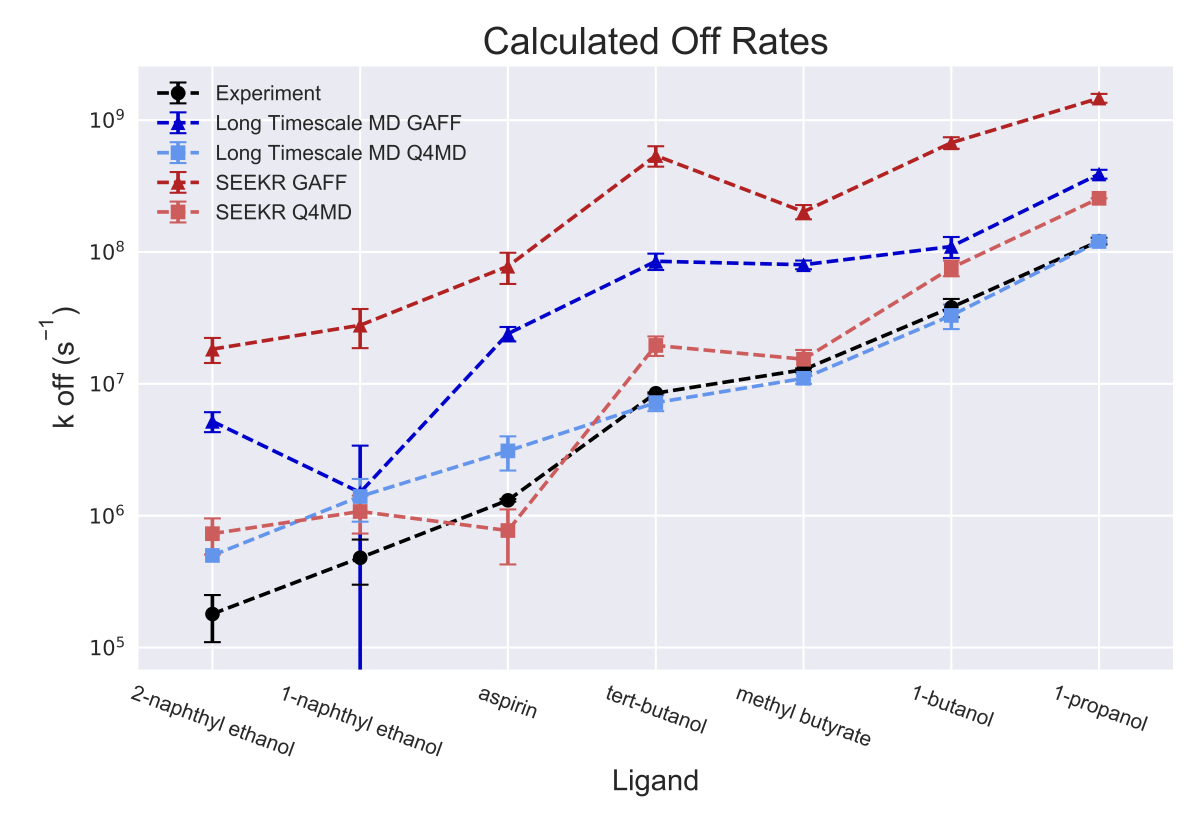
\includegraphics{images/off_scatter_resize.png}
	\caption{}
	\end{subfigure}

	\bigskip
	

	\begin{subfigure}{\linewidth}%<-- changed width
		%\centering
        %\renewcommand\tabularxcolumn[1]{m{#1}}% <-- added
        %\renewcommand\arraystretch{1.3}
        %\setlength\tabcolsep{2pt}% <-- added
    \begin{tabular}{
l  S[table-format = 2.3(3), separate-uncertainty] 
  S[table-format = 2.3(3), separate-uncertainty] 
 }%{\linewidth}%{*{4}{>{\centering\arraybackslash}X}}% <-- changed

\textbf{Method} & \textbf{Kendall} & \textbf{Spearman}  \\
\hline
      SEEKR GAFF      &    0.90(06)           &    0.96(04)            \\ 
      SEEKR Q4MD      &    0.81(09)           &    0.93(05)             \\ 
      Long Timescale MD GAFF      &    0.81(09)           &    0.93(04)                     \\ 
      Long Timescale MD Q4MD      &    01.00(05)           &    1.00(03)                     \\ 
     

    \end{tabular}
        \caption{}
	\end{subfigure}
	\caption{a) Experimental and calculated off rates for SEEKR GAFF and Q4MD forcefields as well as long timescale MD with both forcefields. b) Calculated rank correlation coefficients. Errors are determined with a bootstrapping analysis. }
	\label{fig: off_scatter}
\end{figure}
This trend is seen in both the long timescale MD and SEEKR, 
but is more pronounced in the SEEKR calculations. The Q4MD forcefield, however, 
more accurately reproduces the magnitude of the experimental values with both 
SEEKR and long timescale MD. SEEKR calculations with both Q4MD and GAFF 
forcefields were effective for ranking the compounds by increasing off rates, as evidenced by high rank correlation values.
%SEEKR with GAFF had a Kendall's $\tau = 0.90 \pm 0.06$ only mis-ordering the 
%tert-butanol and methyl butyrate ligands. The rank correlation coefficient for 
%SEEKR with Q4MD was slightly lower, $\tau = 0.81 \pm 0.09$ due to the additional 
%mis-ordering of the naphthyl ethanol ligands. 
The smaller magnitudes of the Q4MD 
values potentially contribute to this forcefield's difficulty to differentiate 
between compounds with similar rates, where the larger values associated with 
the GAFF forcefield allow for more variability in the rate value without changing 
the overall ordering. Both the GAFF and Q4MD forcefields successfully differentiate 
the three tighter binding compounds from the four weaker binding, with the tighter binding compounds 
all having slower off rates and a difference of one order of magnitude between 
the fastest tightly binding compound and the slowest weakly binding compound. This suggests that SEEKR 
could be useful for identifying and separating long residence time ligands from 
shorter residence time ligands and then further discriminating the compounds 
through ranking by \koff.


%%!TEX root = BCD.tex

%%\documentclass[11pt,letterpaper]{article}

%%\usepackage{color}

%%\setlength{\textwidth}{17cm}
%%\setlength{\textheight}{20.5cm}
%%\setlength{\oddsidemargin}{-.1cm}
%%\setlength{\topmargin}{-2 cm}

%%\renewcommand{\baselinestretch}{1.0}

%%\newcommand{\hl}[1]{\textcolor{red}{#1}}
%\newcommand{\hl}[1]{\textbf{#1}}
%\providecommand{\e}[1]{\ensuremath{\times 10^{#1}}}

%%\begin{document}

\begin{table}

\centering
%\resizebox{\textwidth}{!}
{
%\resizebox{\textwidth}{!}{\begin{tabular}{l S@{\pm} S l S @{\,\( \pm \)\,} S l S @{\,\( \pm \)\,} S l S@{\,\( \pm \)\,} S}
\resizebox{\textwidth}{!}{\begin{tabular}{
l S[table-format = 4.2(3)e2, separate-uncertainty] |
l  S[table-format = 4.2(4)e2, separate-uncertainty] |
l S[table-format = 4.2(4)e2, separate-uncertainty]  |
l  S[table-format = 2.3(1)e2, separate-uncertainty] } 

%\multicolumn{8}{c}{\kon rates}
\hline
 \multicolumn{2}{c}{\textbf{Experiment}} & \multicolumn{2}{c}{\textbf{SEEKR}} & \multicolumn{2}{c}{\textbf{Brute Force MD (GAFF)}} & \multicolumn{2}{c}{\textbf{Brute Force MD (Q4MD)}} \\ 
 \hline \hline

 \multirow{2}{*}{\textbf{ligand}} & \koff  & \multirow{2}{*}{\textbf{ligand}}	& \koff  & \multirow{2}{*}{\textbf{ligand}}	& \koff   & \multirow{2}{*}{\textbf{ligand}}	& \koff   \\
 & {(\si{\per\second})} & & {(\si{\per\second})} & & {(\si{\per\second})} & & {(\si{\per\second})} \\



 \hline

2-naphthylethanol &	1.8(7)e6 &	\color{red}{1-naphthylethanol} & 	0.87(34)e6 &	 \color{red}{1-naphthylethanol}	& 1.50(190)e6 & 	2-naphthylethanol	& 0.5  \\
 1-naphthylethanol & 0.48(18)e6 & 	\color{red}{2-naphthylethanol} &	3.43(72)e6	& \color{red}{2-naphthylethanol}	& 5.20(90)e6	 & 1-naphthylethanol& 	1.4(5)e6 \\
aspirin & 	1.31(3)e6 &	aspirin & 	49.31(710)e6 & 	aspirin &	24.00(300)e6 & 	aspirin & 	3.1(9)e6 \\
\textit{tert}-butanol	& 8.50(10)e6 &	\color{red}{methyl butyrate} &	158.35(1550)e6 &	\color{red}{methyl butyrate} &	80.00(600)e6	& \textit{tert}-butanol &	7.2(10)e6 \\
methyl butyrate &	12.80(30)e6 & 	\color{red}{\textit{tert}-butanol} &	258.74(2793)e6 &	\color{red}{\textit{tert}-butanol} &	85.00(1200)e6 &	methyl butyrate &	11(1)e6 \\
1-butanol &	38.00(600)e6 &	1-butanol &	512.16(3745)e6 &	1-butanol &	110.00(2000)e6 &	1-butanol &	33(7)e6 \\
1-propanol &	121.00(700)e6 &	1-propanol &	1495.42(7686)e6 &	1-propanol &	390.00(3000)e6 &	1-propanol&	120(2)e6 \\
\hline

&&\si{\tau} & 0.81(5) & \si{\tau} & 0.81(9) & \si{\tau} & 1.00(4) \\

\hline

\end{tabular}}
}
\caption{ Comparison of \koff values from experiment, SEEKR calculations, and brute force MD simulations with two different forcefields\cite{Tang2017}.
For each method, guest molecules are ranked in order of increasing rates. Ligands that are ordered incorrectly with respect to experiment are colored red. Kendall rank correlation coefficients (\si{\tau}) are also reported for each method.}
\label{table:koff-results}
\end{table}

%%\end{document} %add Q4MD and correct values if using

%\subsubsection*{Binding Free Energy}
\par An additional benefit of kinetics calculations with SEEKR is that binding 
free energies can also be obtained from the same simulations (Fig.~\ref{fig:dg_scatter}). 
\begin{figure}
	\begin{subfigure}{\linewidth}
	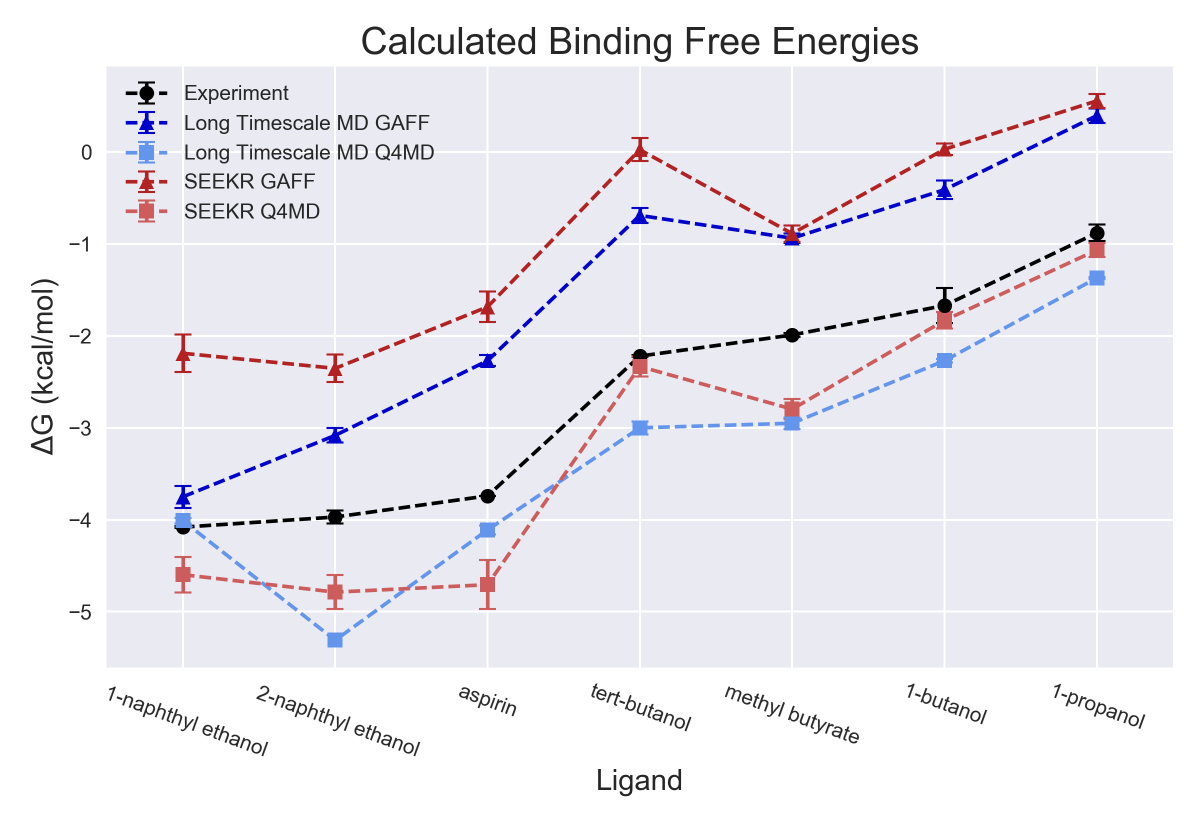
\includegraphics{images/dg_scatter_resize.png}
	\caption{}
	\end{subfigure}
	\bigskip
	\begin{subfigure}{\linewidth}%<-- changed width
		\centering
        %\renewcommand\tabularxcolumn[1]{m{#1}}% <-- added
        %\renewcommand\arraystretch{1.3}
        %\setlength\tabcolsep{2pt}% <-- added
	    \begin{tabular}{
	    	l  S[table-format = 2.3(3), separate-uncertainty] 
	  		S[table-format = 2.3(3), separate-uncertainty] 
	 	}%{\linewidth}%{*{4}{>{\centering\arraybackslash}X}}% <-- changed

			\textbf{Method} & \textbf{Kendall} & \textbf{Spearman}  \\
			\hline
	        SEEKR GAFF      &    0.88(08)           &    0.96(05)            \\ 
	        SEEKR Q4MD      &    0.73(10)           &    0.89(06)             \\ 
	        Long Timescale MD GAFF      &    0.90(07)           &    0.96(04)                     \\ 
	        Long Timescale MD Q4MD      &    0.87(11)           &    0.94(06)                     \\ 
	     

	    \end{tabular}
        \caption{}
	\end{subfigure}
	\caption{a) Experimental and calculated binding free energies for SEEKR GAFF and Q4MD forcefields as well as long timescale MD with both forcefields. b) Calculated rank correlation coefficients. Errors are determined with a bootstrapping analysis. }
	
	\label{fig:dg_scatter}
\end{figure}
Binding free energies calculated using the rate constants %$\Delta G= -RTln(k_{\textrm{on}}/k_{\textrm{off}})$, 
are most heavily influenced by the \koff for these ligands, as this value is more variable, where 
the \kon's for all ligands are more similar. Therefore, similar trends are observed 
for the calculated binding free energies as were observed for the off rates.
Binding free energies can also be calculated using the stationary probabilities 
for each milestone, rather than the rate constants, and produce similar results.
The GAFF forcefield consistently underestimates the binding free energies in both 
SEEKR and the long timescale MD, resulting from the consistent underestimation 
of the magnitudes of the \koff's. The magnitudes of the binding free 
energies calculated using Q4MD are in much better agreement with the experimental 
values, differing by 1 kcal or less. SEEKR with both Q4MD and GAFF successfully 
differentiates the three known tighter binding compounds from the four weaker binding compounds.
%Experimentally, there is a difference of 1.52 kcal/mol between the two groups.
%The GAFF calculation underestimates this difference, calculating a difference of 
%$0.79 \pm 0.19$ kcal/mol between the aspirin and methyl butyrate ligands while SEEKR 
%with Q4MD slightly overestimates the difference, calculating a difference of 
%$1.8 \pm 0.11$  kcal/mol between 1-naphthyl ethanol and methyl butyrate. Again 
%this suggests that SEEKR is a useful tool for differentiating tight binders 
%from weaker binders. 
SEEKR can also further discriminate ligands 
by its effective ranking %of ligands 
by binding free energies, demonstrated by high rank correlation values.

%producing Kendal 
%rank correlation values of $0.88 \pm 0.08$ for GAFF and $0.73 \pm 0.1$ for Q4MD.



%%!TEX root = BCD.tex

%%\documentclass[11pt,letterpaper]{article}

%%\usepackage{color}

%%\setlength{\textwidth}{17cm}
%%\setlength{\textheight}{20.5cm}
%%\setlength{\oddsidemargin}{-.1cm}
%%\setlength{\topmargin}{-2 cm}

%%\renewcommand{\baselinestretch}{1.0}

%%\newcommand{\hl}[1]{\textcolor{red}{#1}}
%\newcommand{\hl}[1]{\textbf{#1}}
%\providecommand{\e}[1]{\ensuremath{\times 10^{#1}}}

%%\begin{document}

\begin{table}

\centering
%\resizebox{\textwidth}{!}
{
\resizebox{\textwidth}{!}{\begin{tabular}{
l S[table-format = 1.2(2), separate-uncertainty] |
l  S[table-format = 1.2(2), separate-uncertainty] |
l S[table-format = 1.2(2), separate-uncertainty]  |
l  S[table-format = 1.2(2), separate-uncertainty] }

% \resizebox{\textwidth}{!}{\begin{tabular}{
% l S[table-format = 4.2(4)e8, separate-uncertainty, table-figures-uncertainty = 4.2] |
% l  S[table-format = 4.2e8, separate-uncertainty, table-figures-uncertainty = 4.2] |
% l S[table-format = 4.2e8, separate-uncertainty, table-figures-uncertainty = 4.2]  |
% l  S[table-format = 4.2e8, separate-uncertainty, table-figures-uncertainty = 4.2] |}

%\multicolumn{8}{c}{\kon rates}
\hline

 \multicolumn{2}{c}{\textbf{Experiment}} & \multicolumn{2}{c}{\textbf{SEEKR}} & \multicolumn{2}{c}{\textbf{Brute Force MD (GAFF)}} & \multicolumn{2}{c}{\textbf{Brute Force MD (Q4MD)}} \\ 
 \hline \hline


 \multirow{2}{*}{\textbf{ligand}} & $\Delta G$  & \multirow{2}{*}{\textbf{ligand}}	& $\Delta G$  & \multirow{2}{*}{\textbf{ligand}}	& $\Delta G$   & \multirow{2}{*}{\textbf{ligand}}	& $\Delta G$   \\
 & {(\si{\kcal\per\mol})} & & {(\si{\kcal\per\mol})} & & {(\si{\kcal\per\mol})} & & {(\si{\kcal\per\mol})} \\



 \hline

1-naphthylethanol & -4.08(1) & 1-naphthylethanol & -4.33(24) & 1-naphthylethanol	& -3.75(12) & \color{red}{2-naphthylethanol} & -5.31 \\ 

2-naphthylethanol &	-3.97(7)	& 2-naphthylethanol 	& -3.67(13)	& 2-naphthylethanol		& -3.08(8) & \color{red}{aspirin} 	& -4.11(5) \\

aspirin &	-3.74(00) 	& aspirin &	-2.07(9) 	& aspirin &	-2.27(6) 	& \color{red}{1-naphthylethanol} &	-4.01(03) \\

\textit{tert}-butanol & -2.22(1) &	\color{red}{methyl butyrate} & -1.15(7) &	\color{red}{methyl butyrate} &	-0.94(5) & \textit{tert}-butanol & -3.00(7) \\

 methyl butyrate & -1.99(2) & \color{red}{\textit{tert}-butanol} & -0.61(7) & \color{red}{\textit{tert}-butanol} & -0.69(8) &	methyl butyrate & -2.95(6) \\

1-butanol & -1.67(19) & 1-butanol &	-0.38(6) & 1-butanol & -0.41(10) & 1-butanol &	-2.27(2) \\


1-propanol & -0.88(9) & 1-propanol & 0.49(6) &	1-propanol & 0.40(8) &	1-propanol &	-1.37(1) \\

\hline
&&\si{\tau} & 0.90(7) & \si{\tau} & 0.90(7) & \si{\tau} & 0.87(10) \\

\hline

\end{tabular}}
}
\caption{ Comparison of \kon values from experiment, SEEKR calculations, and brute force MD simulations with two different forcefields\cite{Tang2017}.
For each method, guest molecules are ranked in order of increasing rates.Ligands that are ordered incorrectly with respect to experiment are colored red. Kendall rank correlation coefficients (\si{\tau}) are also reported for each method.}
\label{table:dG-results}
\end{table}

%%\end{document}


\par A key aspect of future development of the SEEKR software is the systematic 
development of methodological best-practices as well as the elucidation of the 
sensitivity of calculated kinetic parameters to various SEEKR input conditions.

%\subsubsection*{Sampling}
While it is possible to determine the kinetics for small systems like 
$\beta$-cyclodextrin using conventional long timescale MD simulations, increasing 
system size soon makes this inefficient or even impossible. 
%The advantage of the 
%SEEKR approach is twofold; 1) reducing the  simulation time required to obtain 
%accurate kinetics and 2) reducing the overall time required for calculations by 
%employing a highly parallel approach. The current bottleneck for SEEKR calculations 
%is obtaining the equilibrium distribution, which still requires relatively long MD simulations on the order of hundreds of nanoseconds per milestone. It is therefore of great interest to reduce the amount 
%of simulation necessary for achieving converged rate values.
The convergence of \kon and \koff were assessed by calculating the rate 
constants as a function of the reversal trajectory number at increasing intervals 
of 50 reversal numbers (with 10 trajectories initiated for each reversal number).
The reversal number is a direct measure of the equilibrium simulation length, as 
reversals are initiated from evenly spaced configurations of the equilibrium distribution.
In general, both the on and off rates appear converged in less than the maximum 
number of reversals available. Approximately half the total reversals 
(4000 of 8000) were sufficient for obtaining reasonably converged rate constants. 
This suggests that the total simulation cost to obtain a similar result could be 
as little as 2 ${\mu}s$ per ligand, rather than 3.8 ${\mu}s$.

%\begin{figure}
\begin{subfigure}{0.3\linewidth}
	\centering
	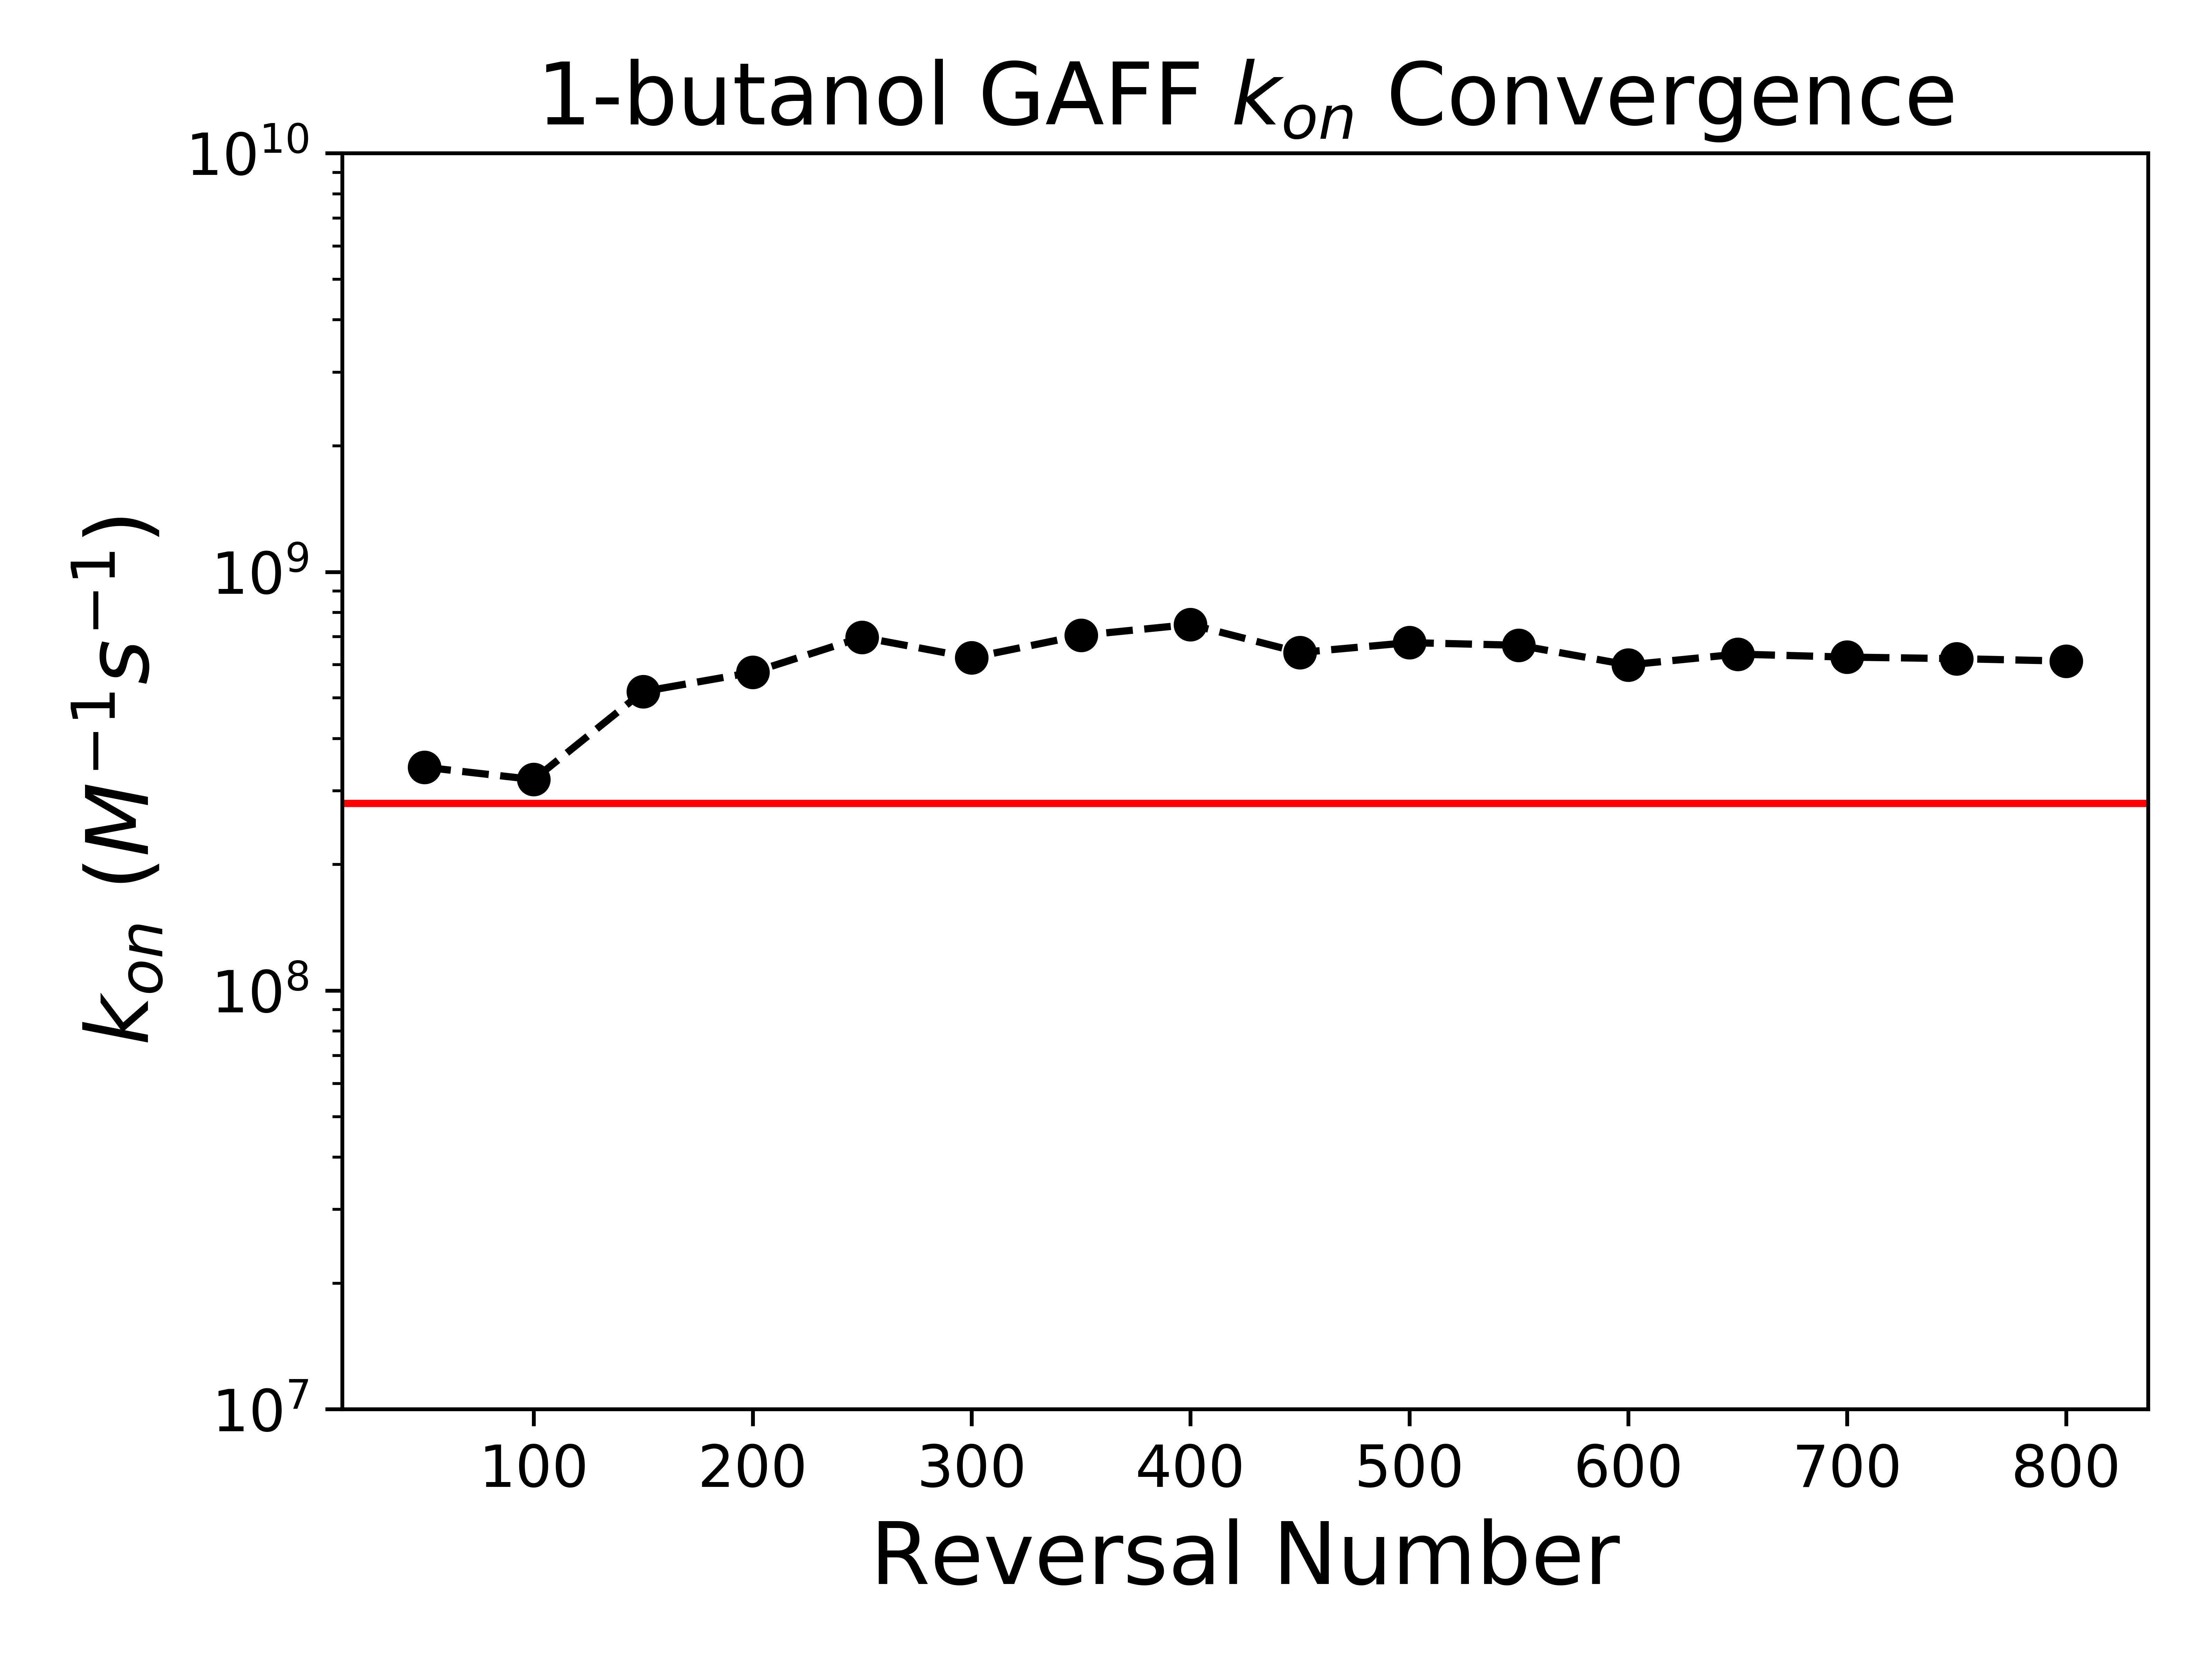
\includegraphics[width=\linewidth]{high_res_images/gaff_rate_conv_images/1-butanol_gaff_on_conv.png}
	\end{subfigure}%
\begin{subfigure}{0.3\linewidth}
		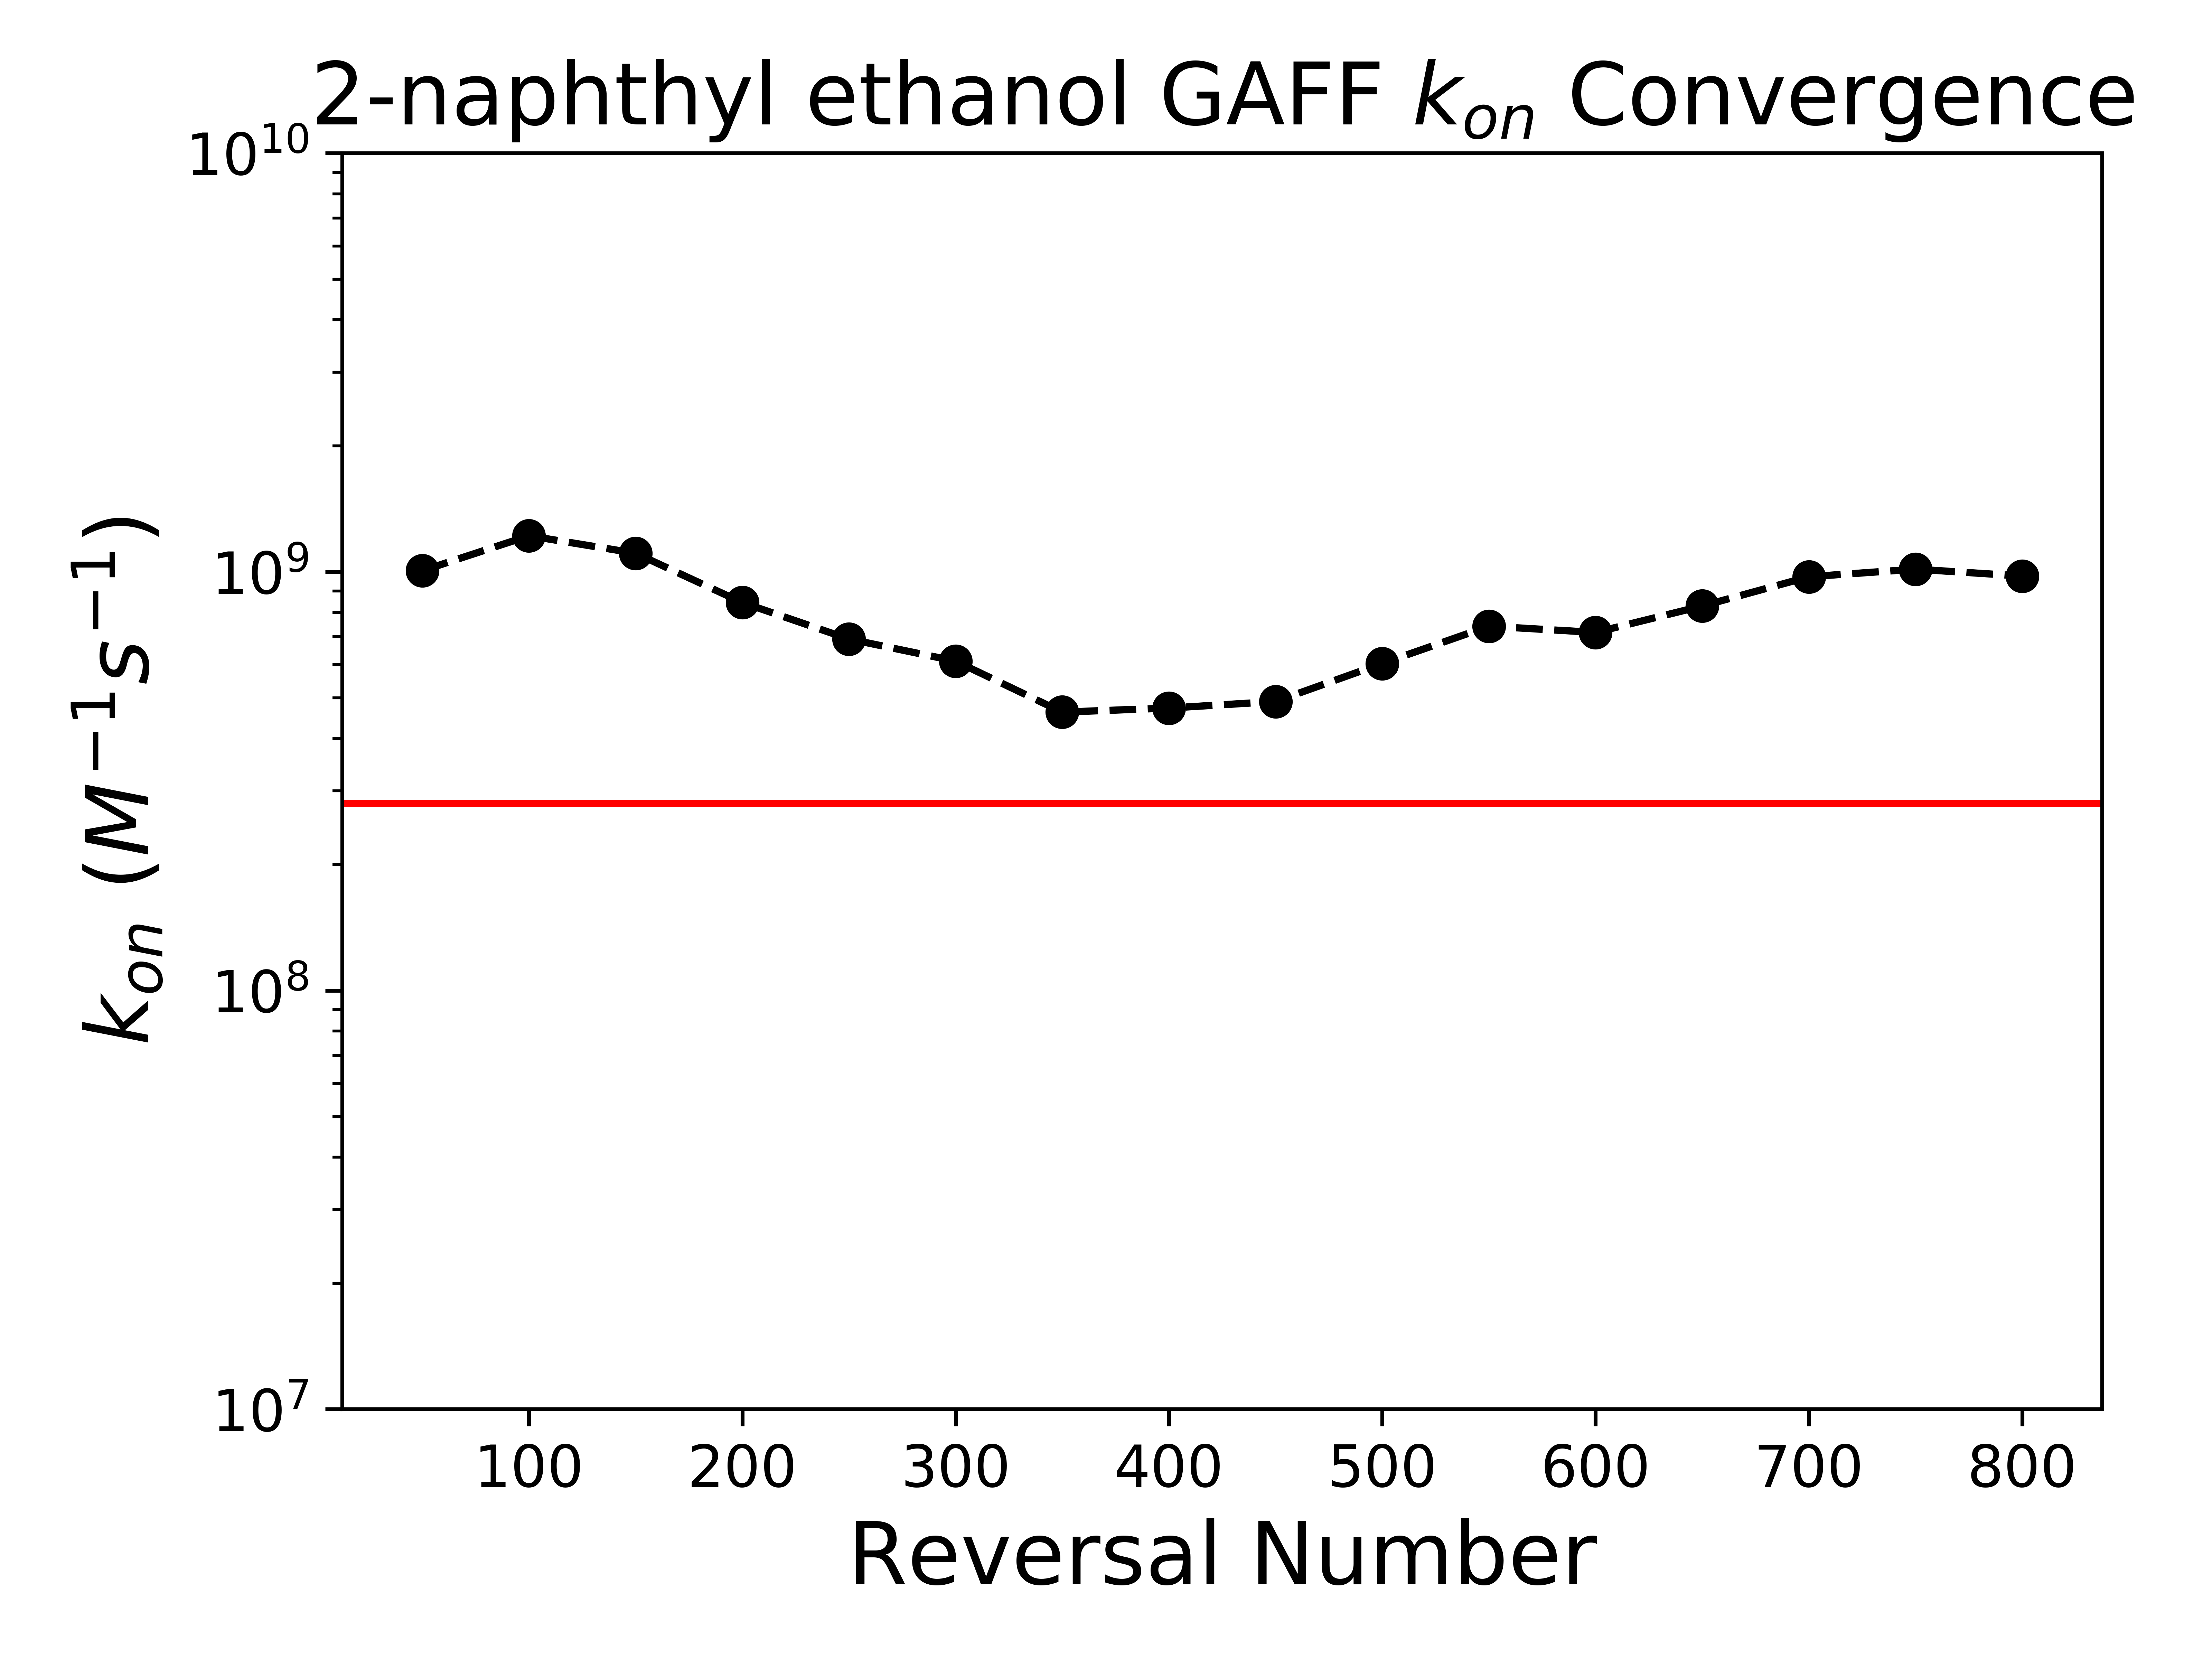
\includegraphics[width=\linewidth]{high_res_images/gaff_rate_conv_images/2-naphthylethanol_gaff_on_conv.png}
\end{subfigure}%
	\begin{subfigure}{0.3\linewidth}
		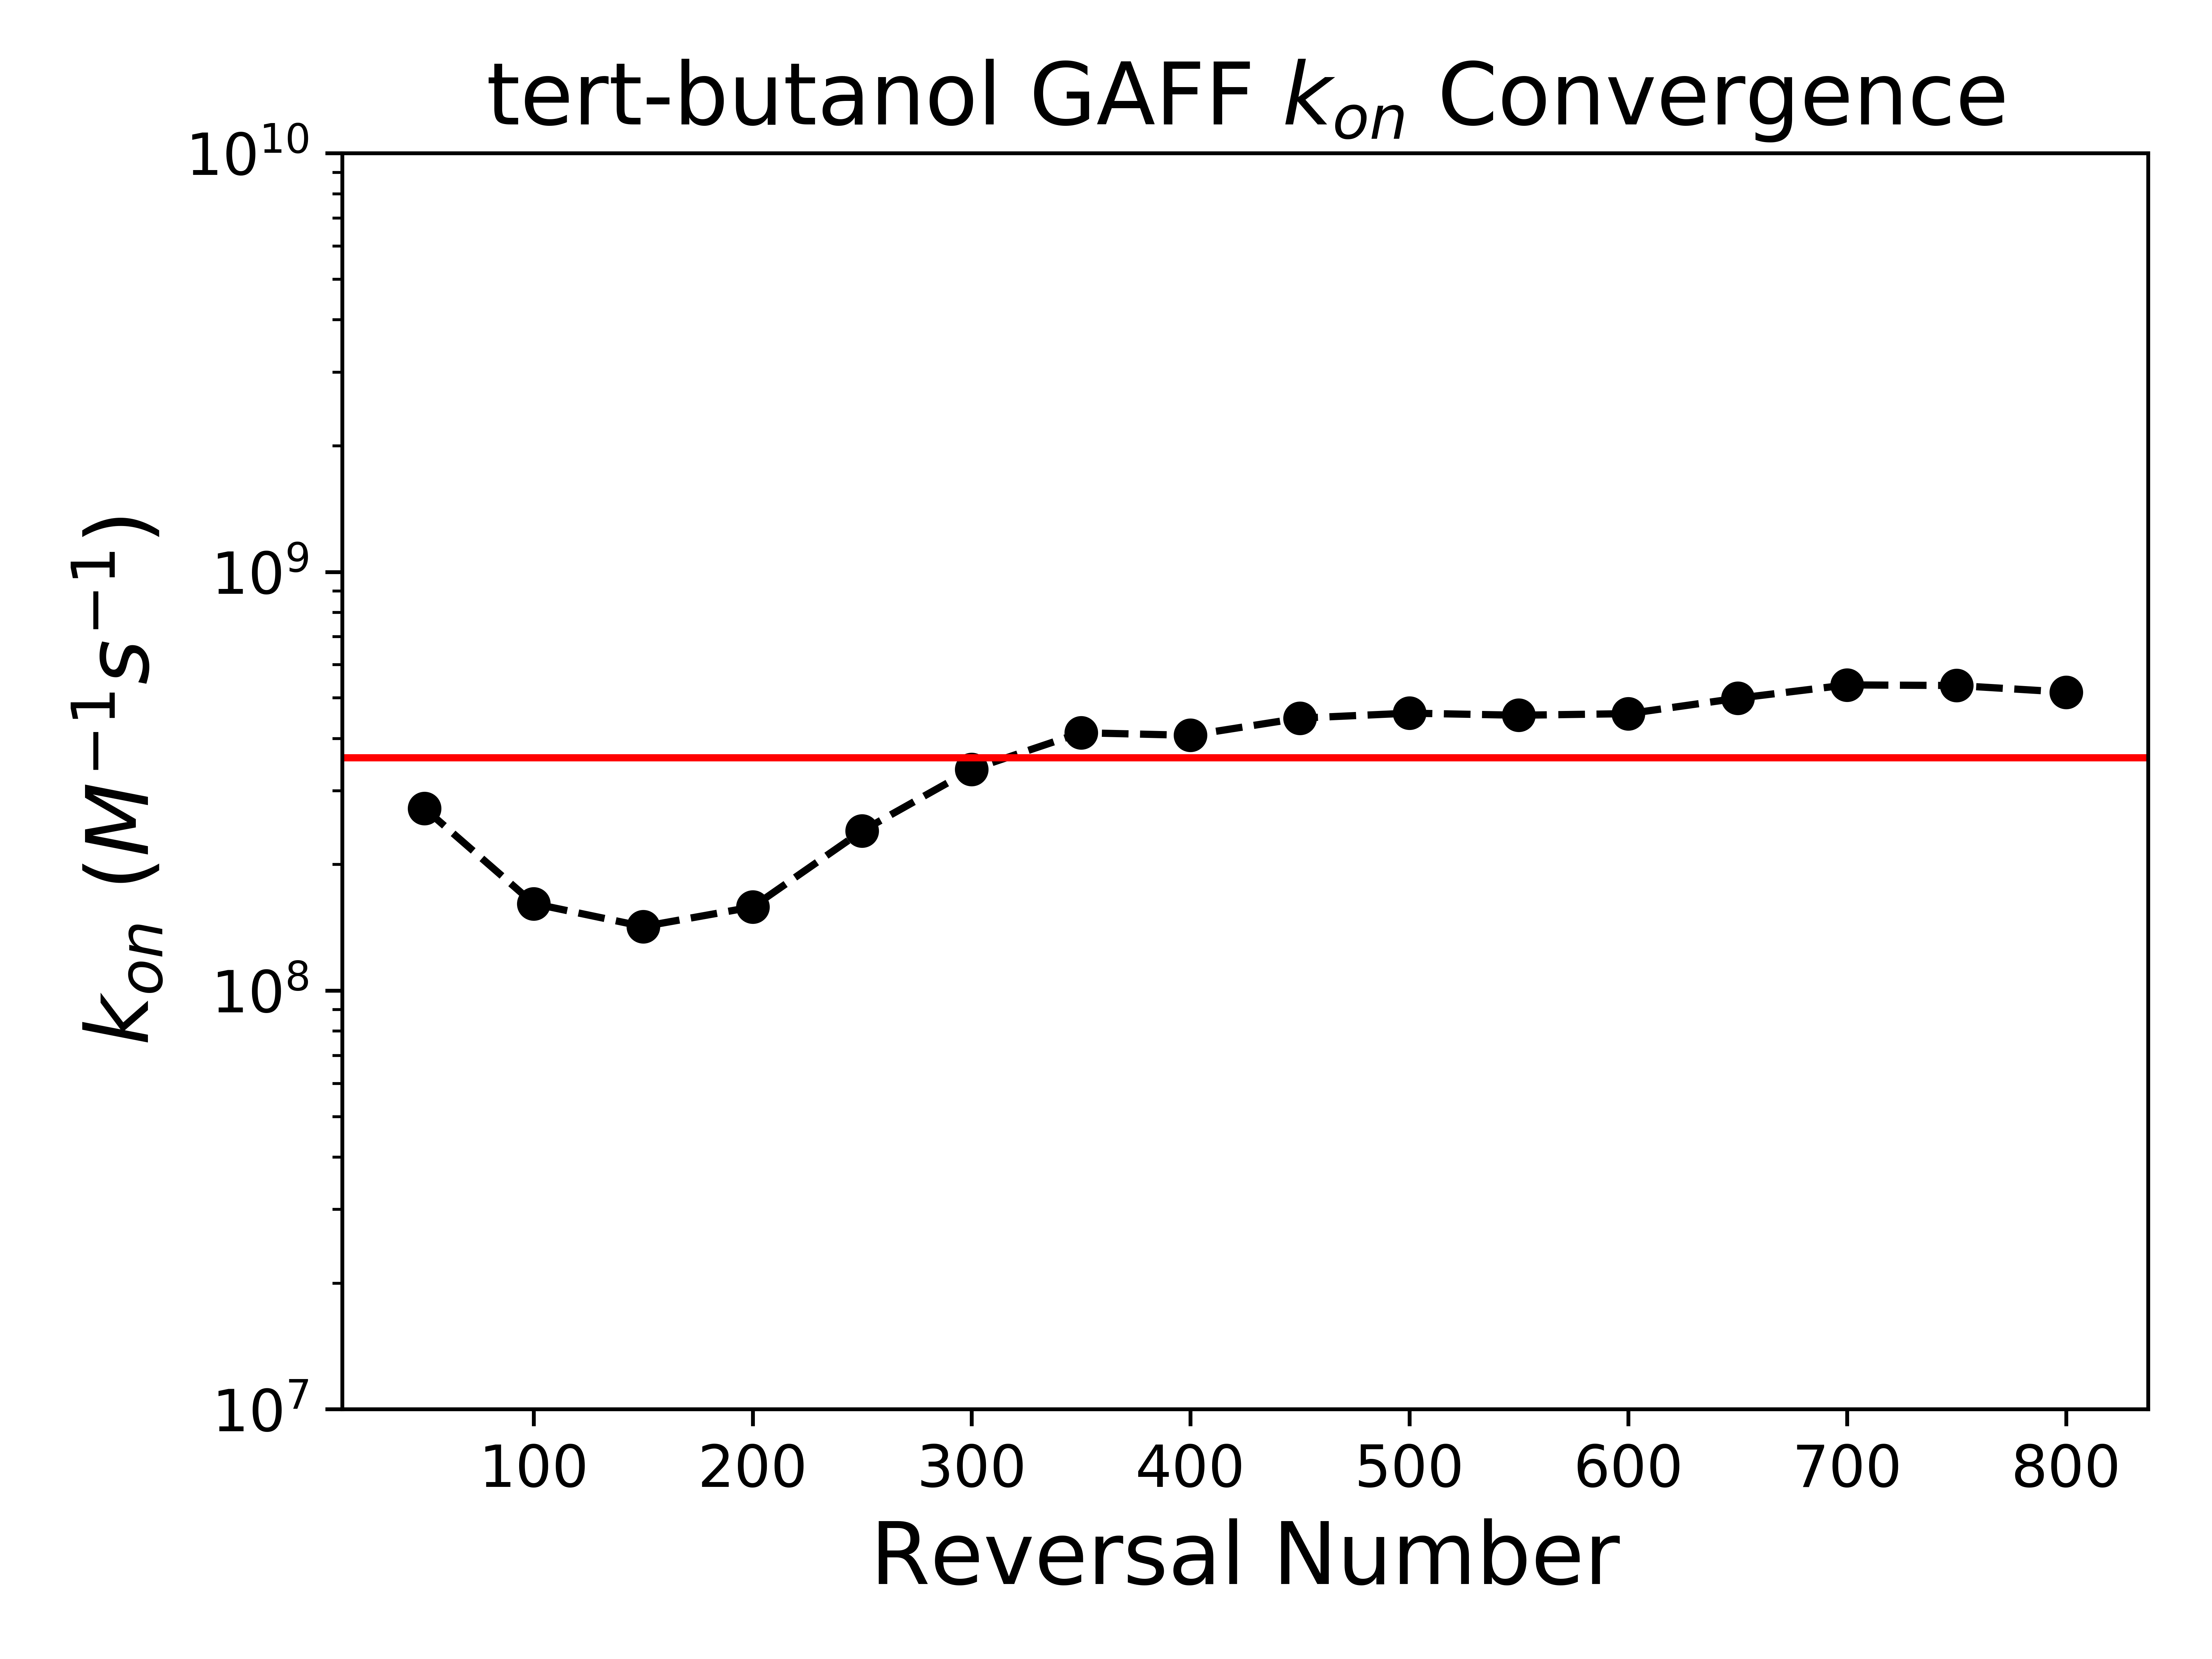
\includegraphics[width=\linewidth]{high_res_images/gaff_rate_conv_images/tert-butanol_gaff_on_conv.png}
	\end{subfigure}
	\begin{subfigure}{0.3\linewidth}
		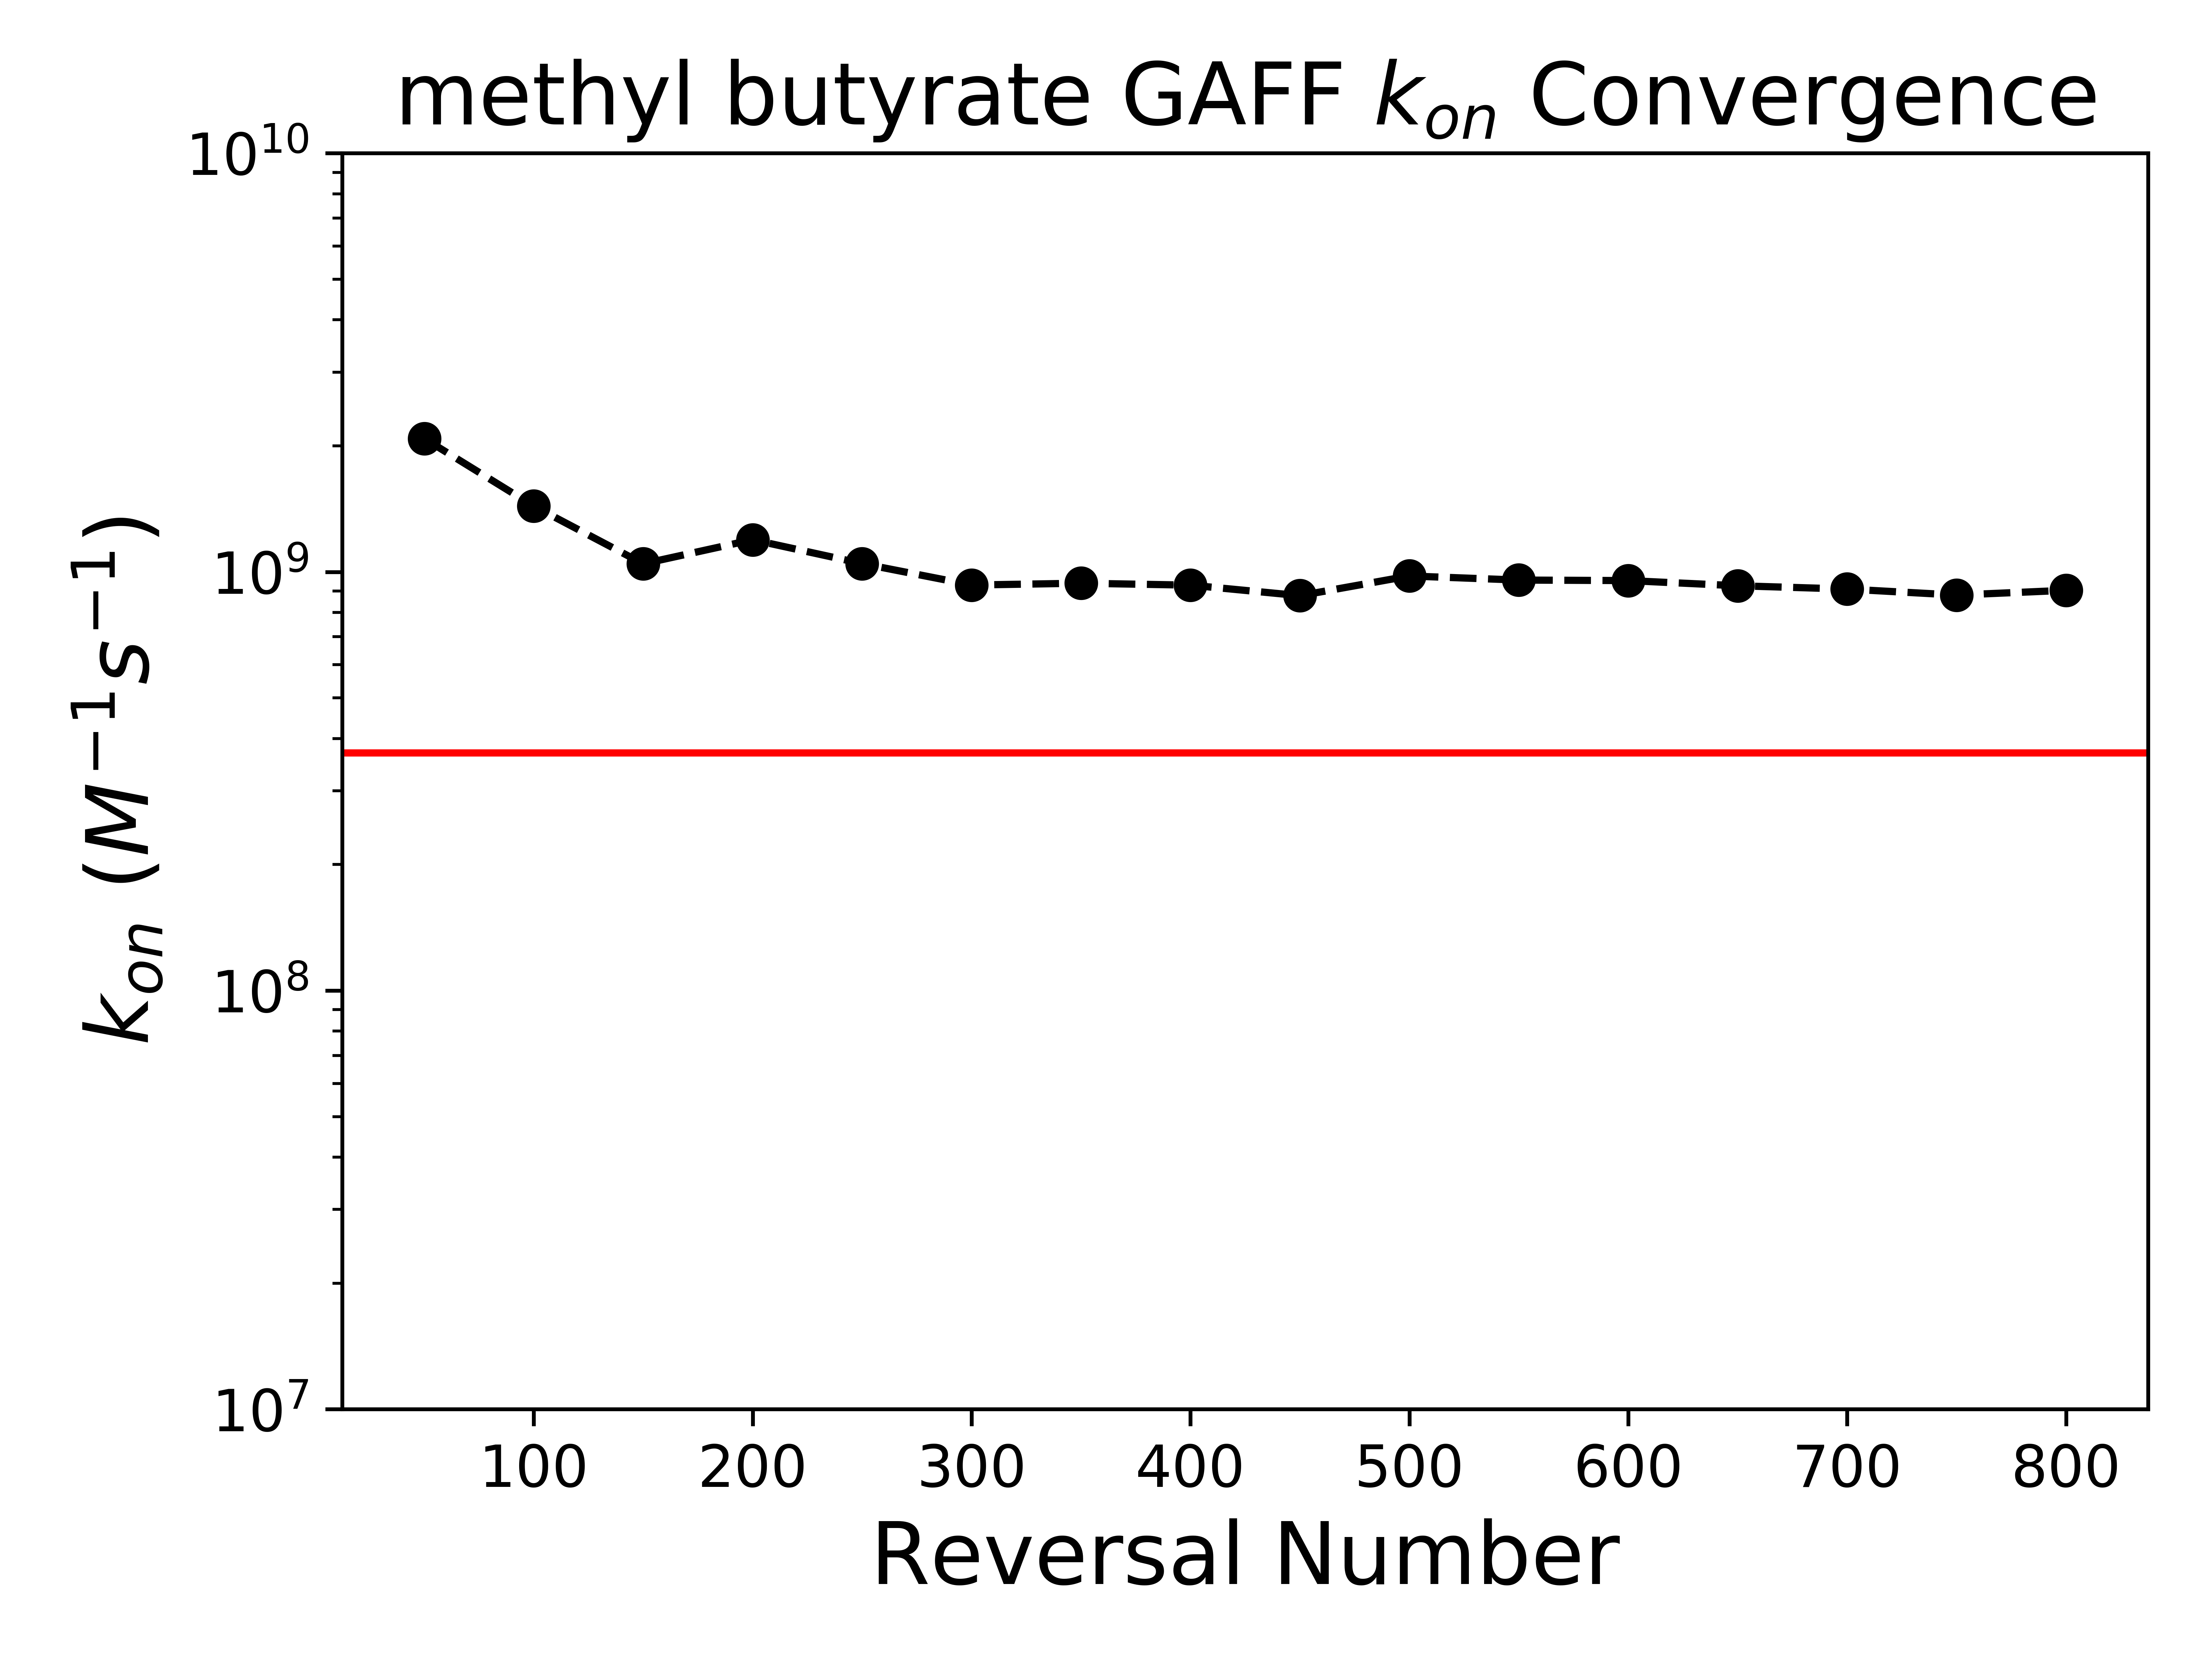
\includegraphics[width=\linewidth]{high_res_images/gaff_rate_conv_images/methylbutyrate_gaff_on_conv.png}
	\end{subfigure}
	\begin{subfigure}{0.3\linewidth}
		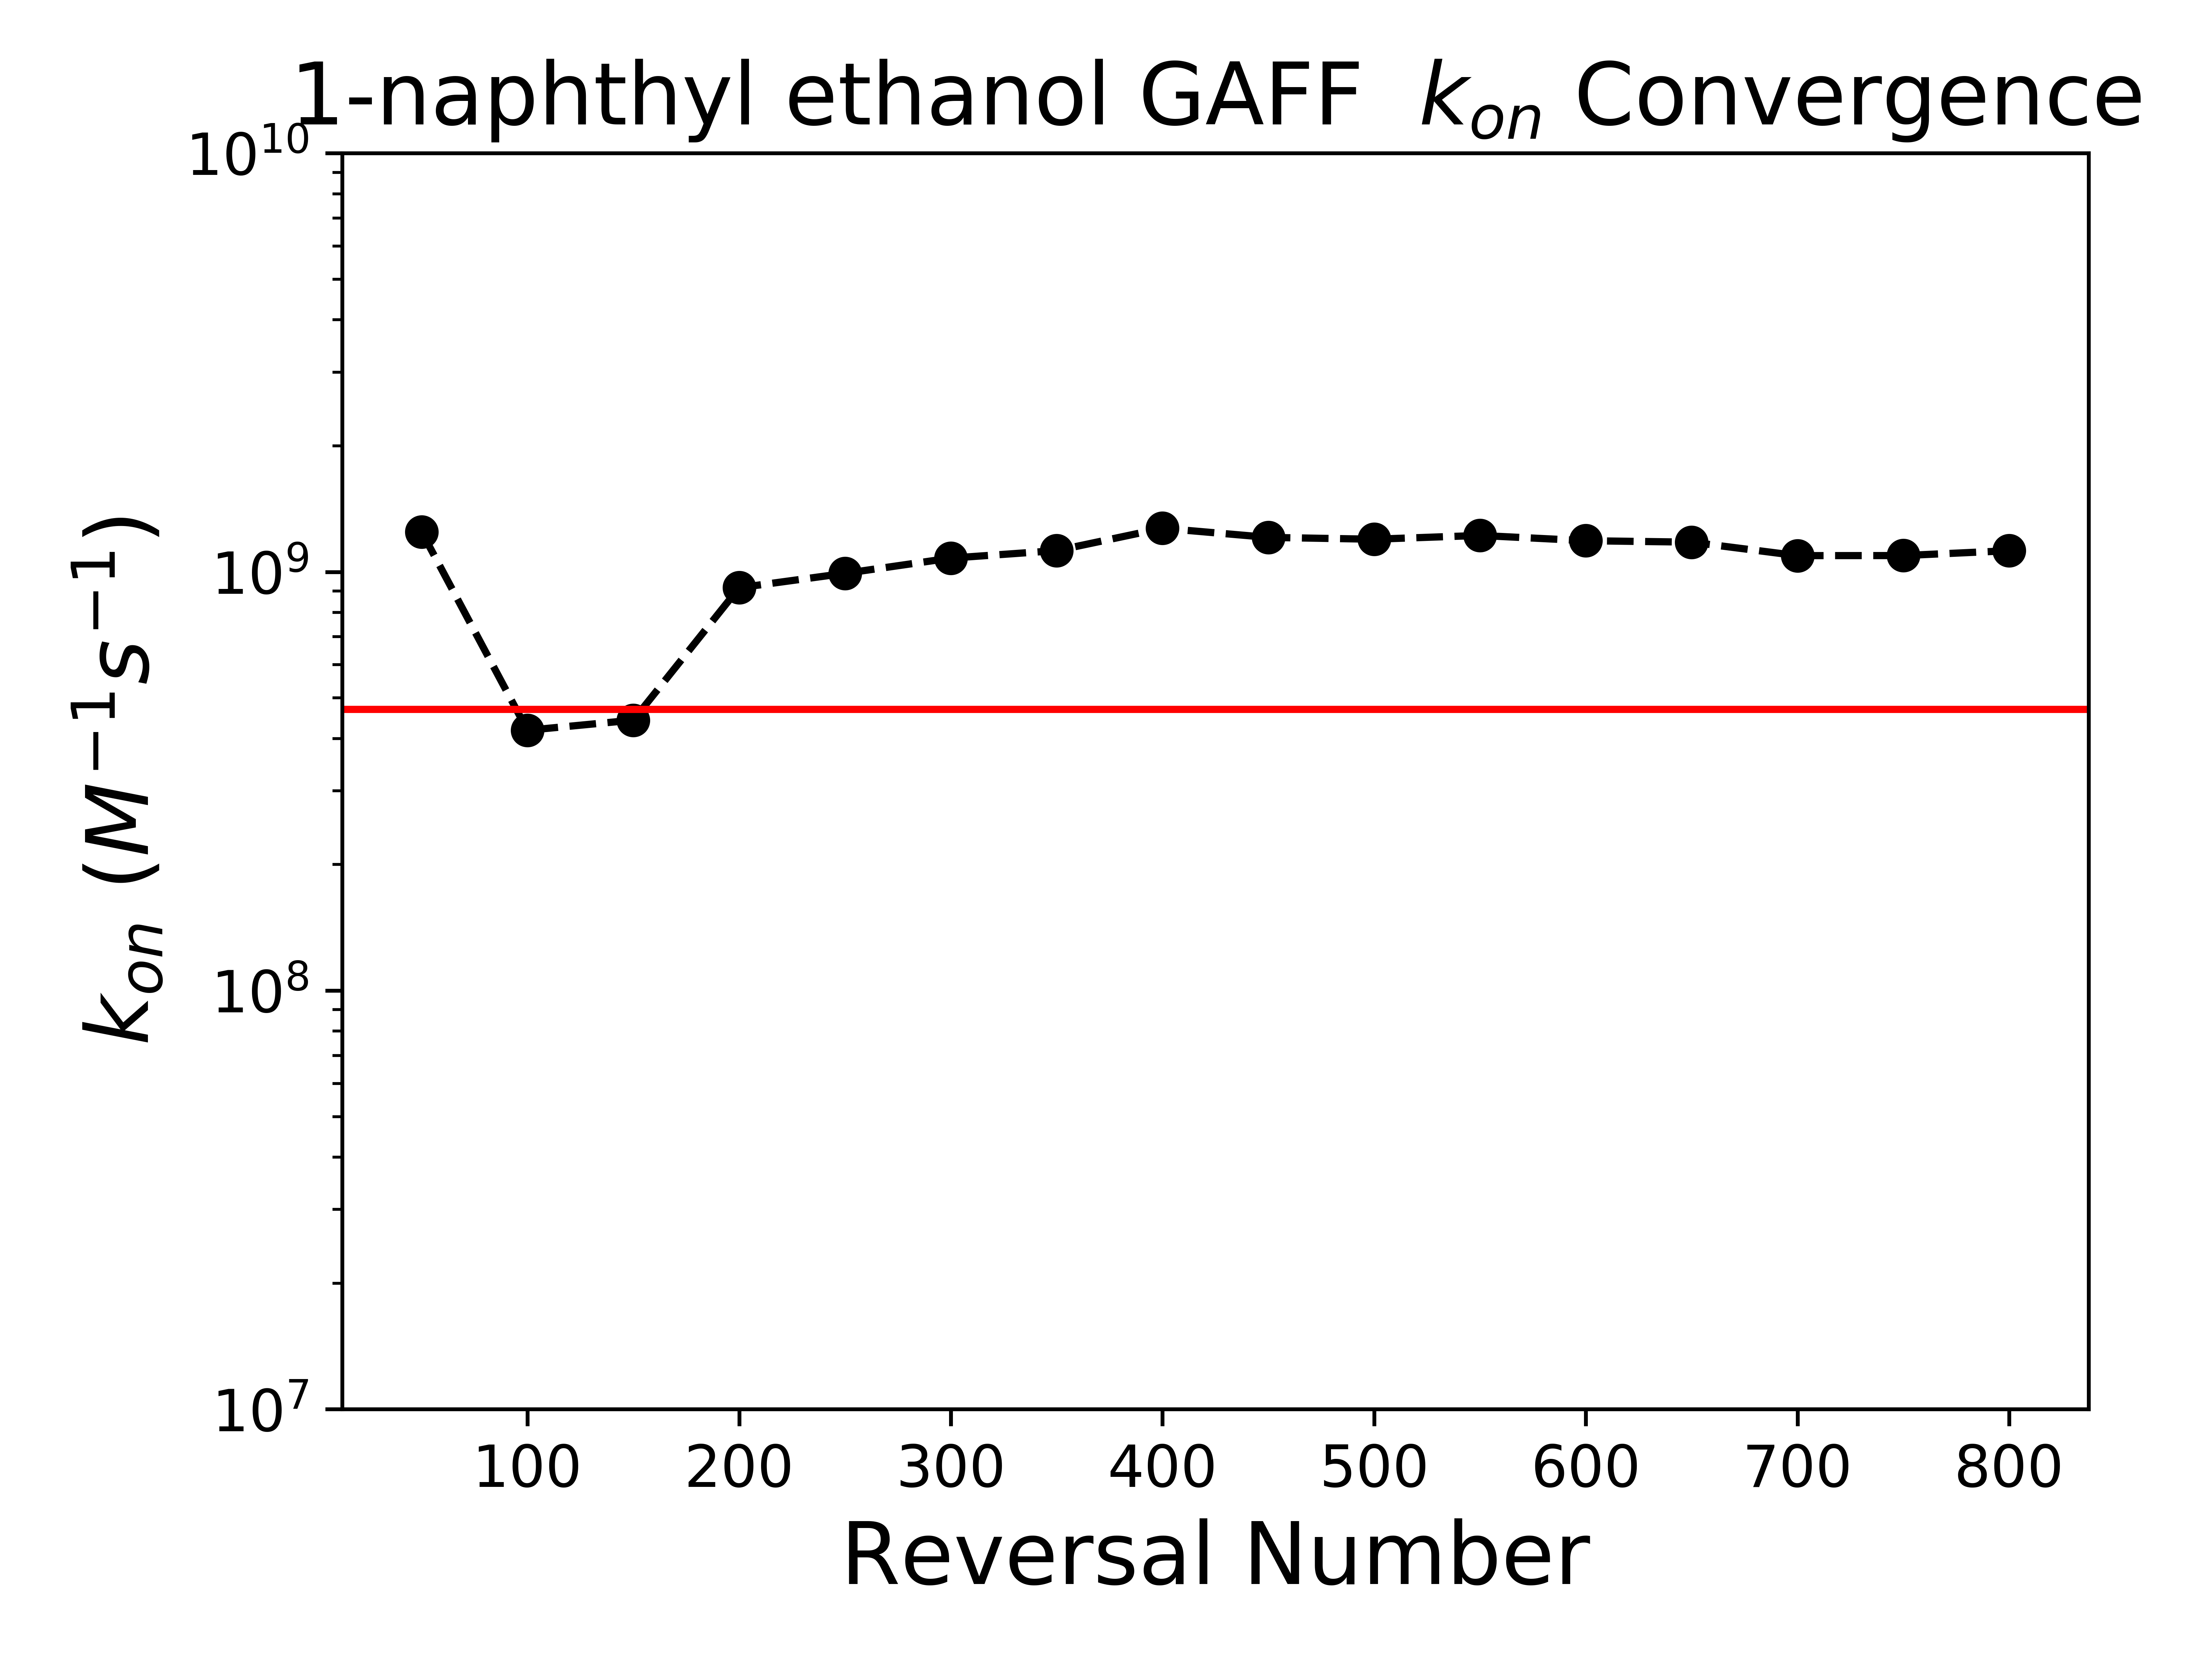
\includegraphics[width=\linewidth]{high_res_images/gaff_rate_conv_images/1-naphthylethanol_gaff_on_conv.png}
	\end{subfigure}
	\begin{subfigure}{0.3\linewidth}
		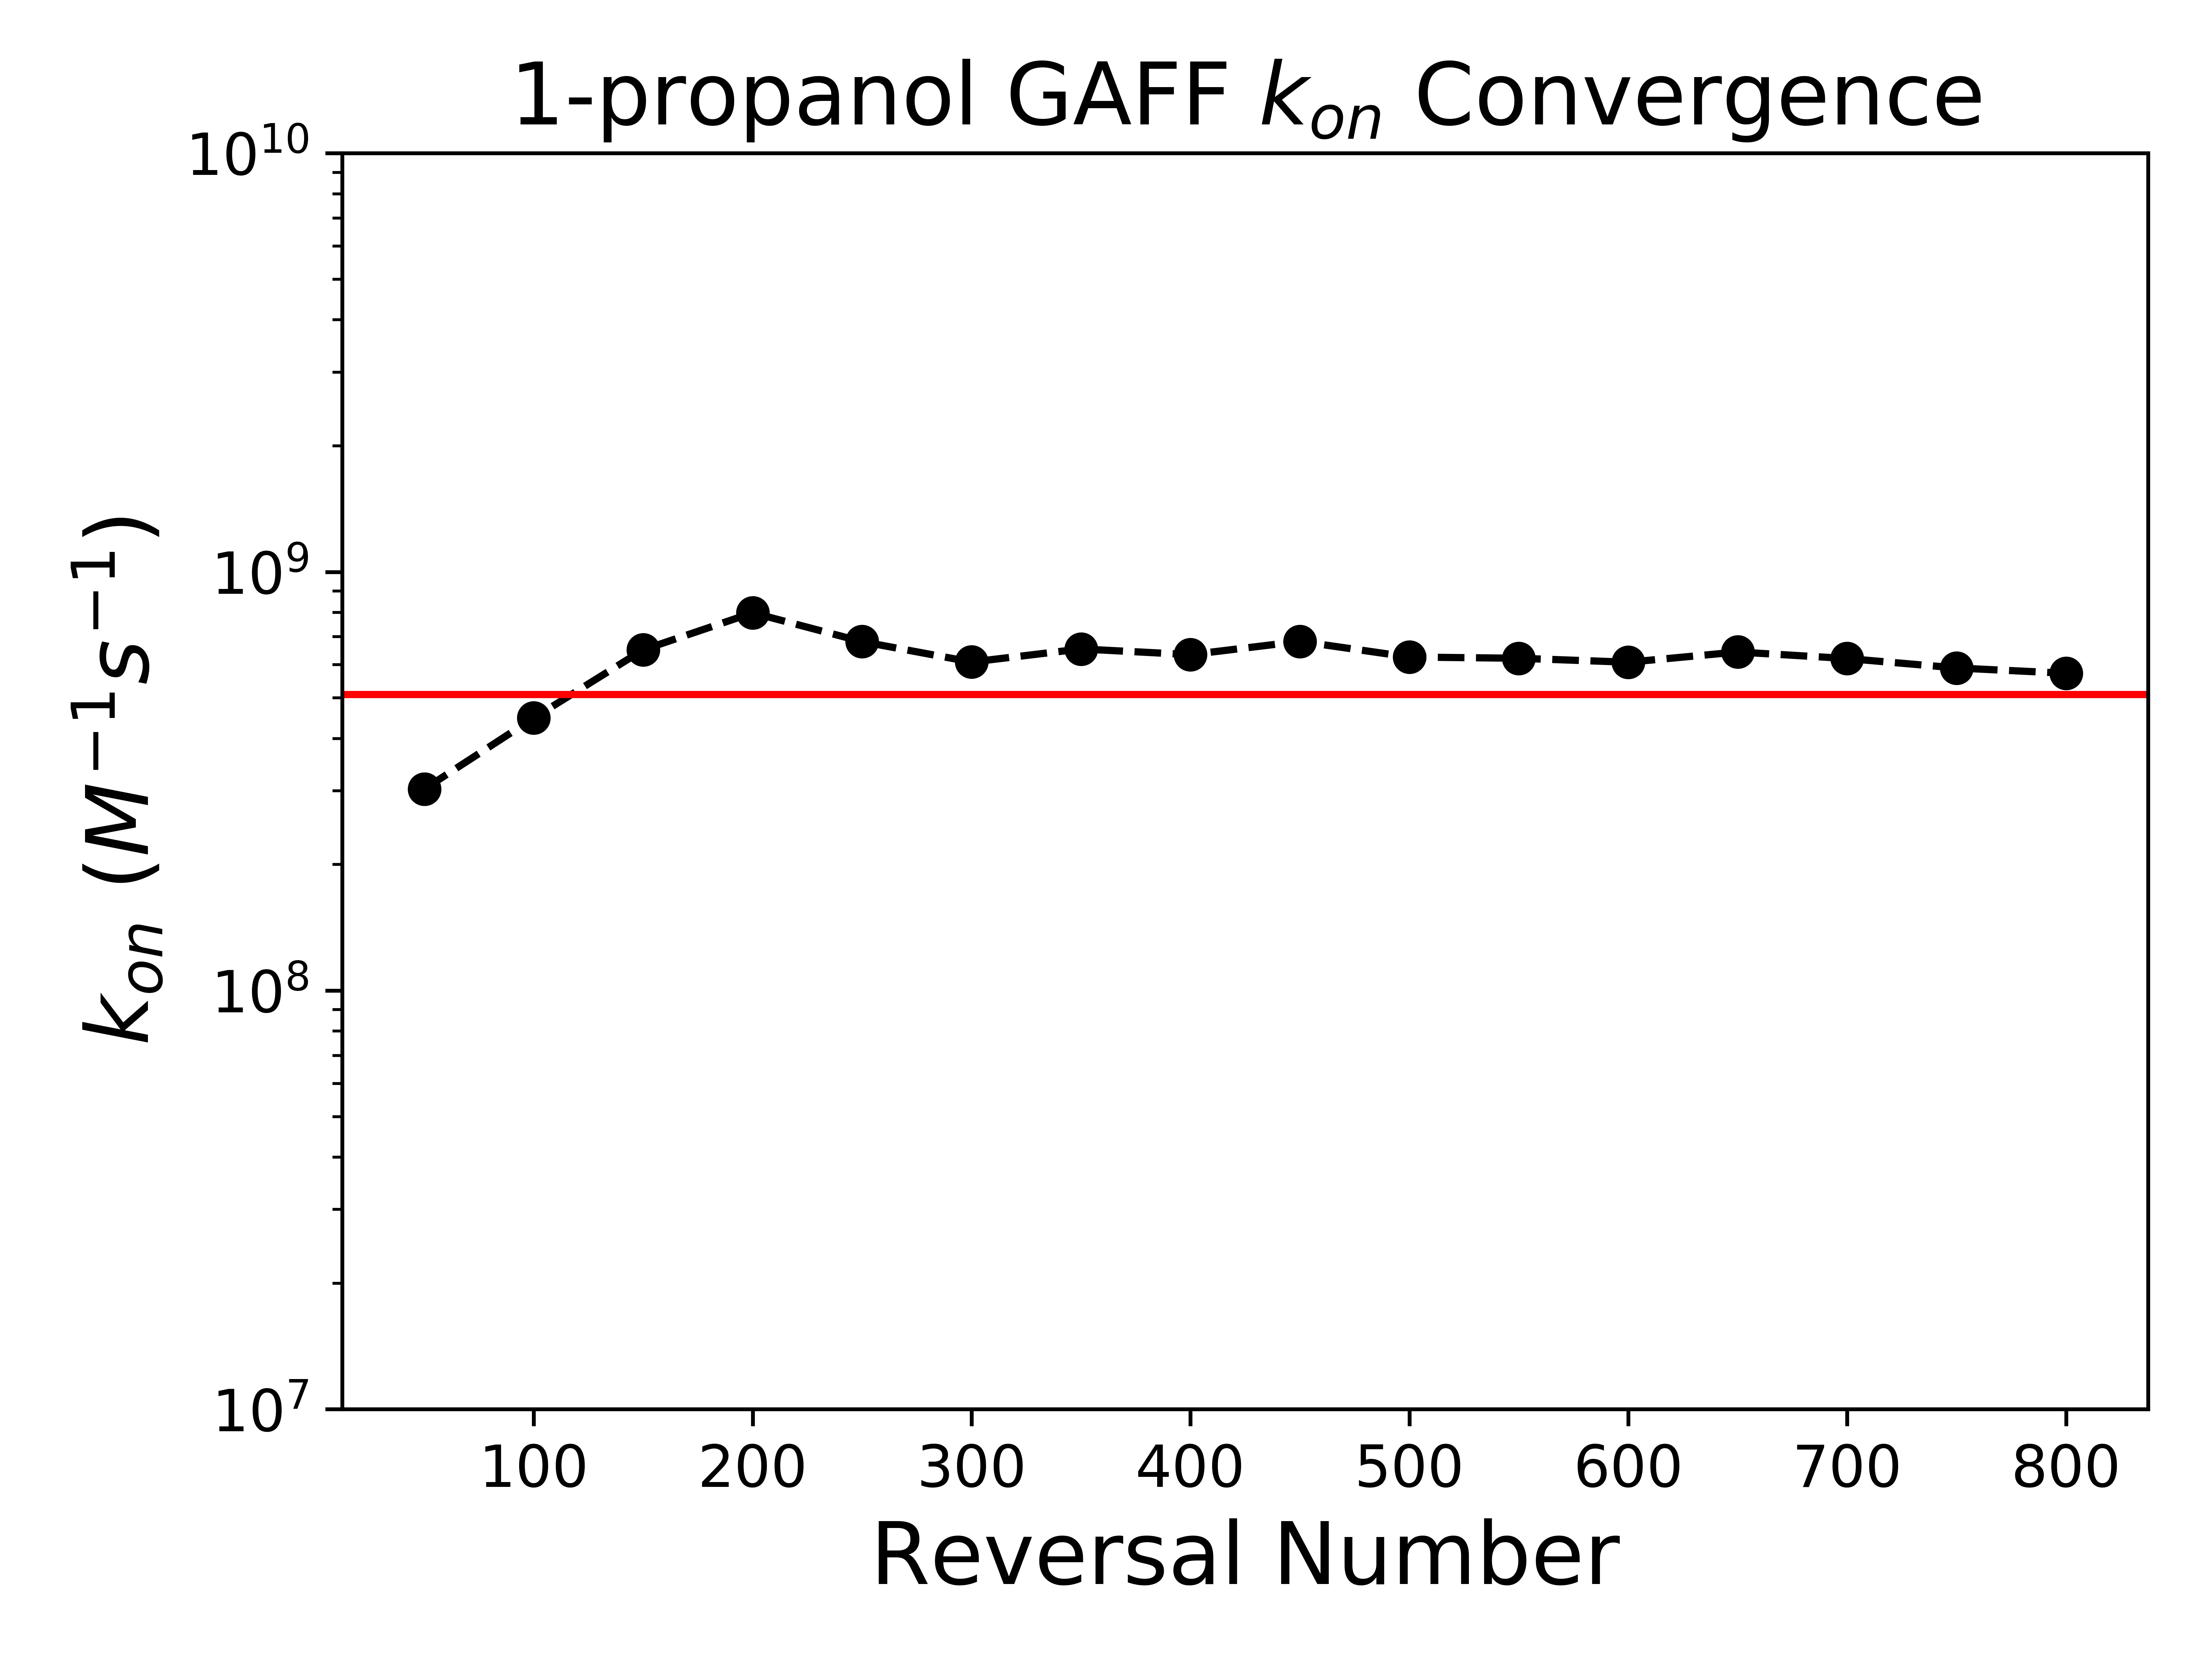
\includegraphics[width=\linewidth]{high_res_images/gaff_rate_conv_images/1-propanol_gaff_on_conv.png}
	\end{subfigure}
	\begin{subfigure}{0.3\linewidth}
		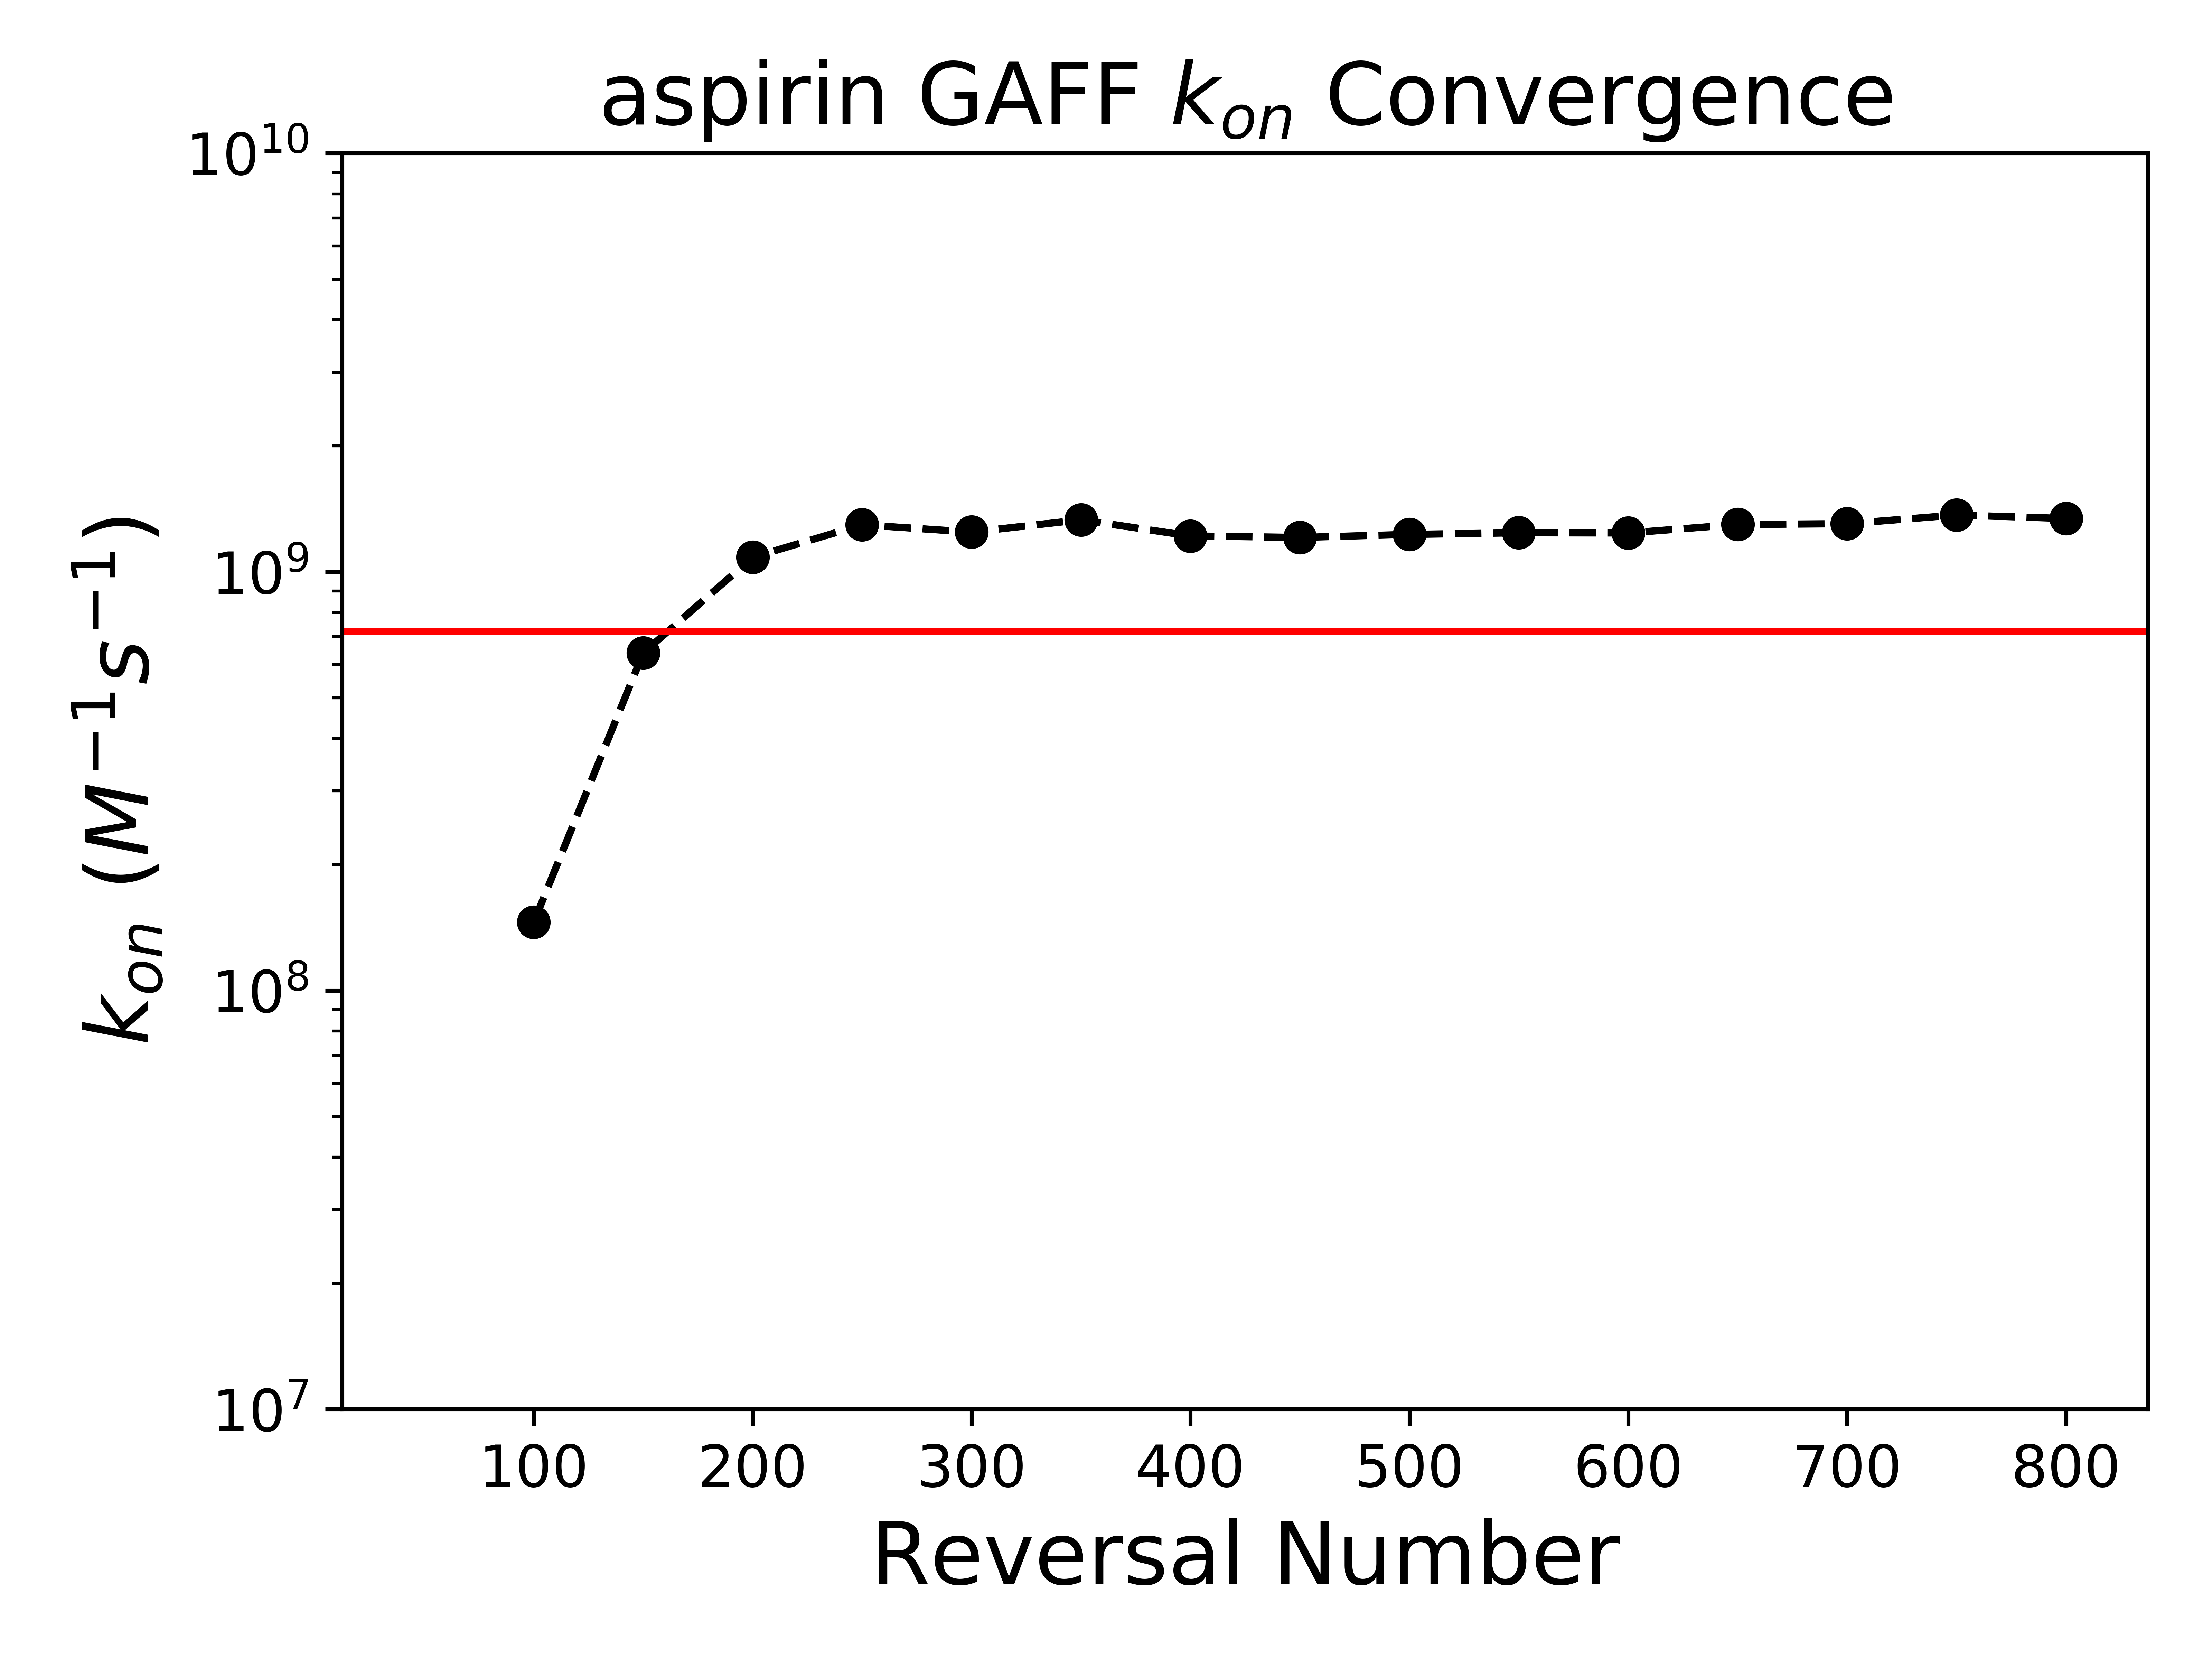
\includegraphics[width=\linewidth]{high_res_images/gaff_rate_conv_images/aspirin_gaff_on_conv.png}
	\end{subfigure}
	\caption{Convergence of on rates as a function of the number of reversals included using the GAFF forcefield}
\end{figure}
%\begin{figure}
\centering
	\begin{subfigure}{0.3\linewidth}
	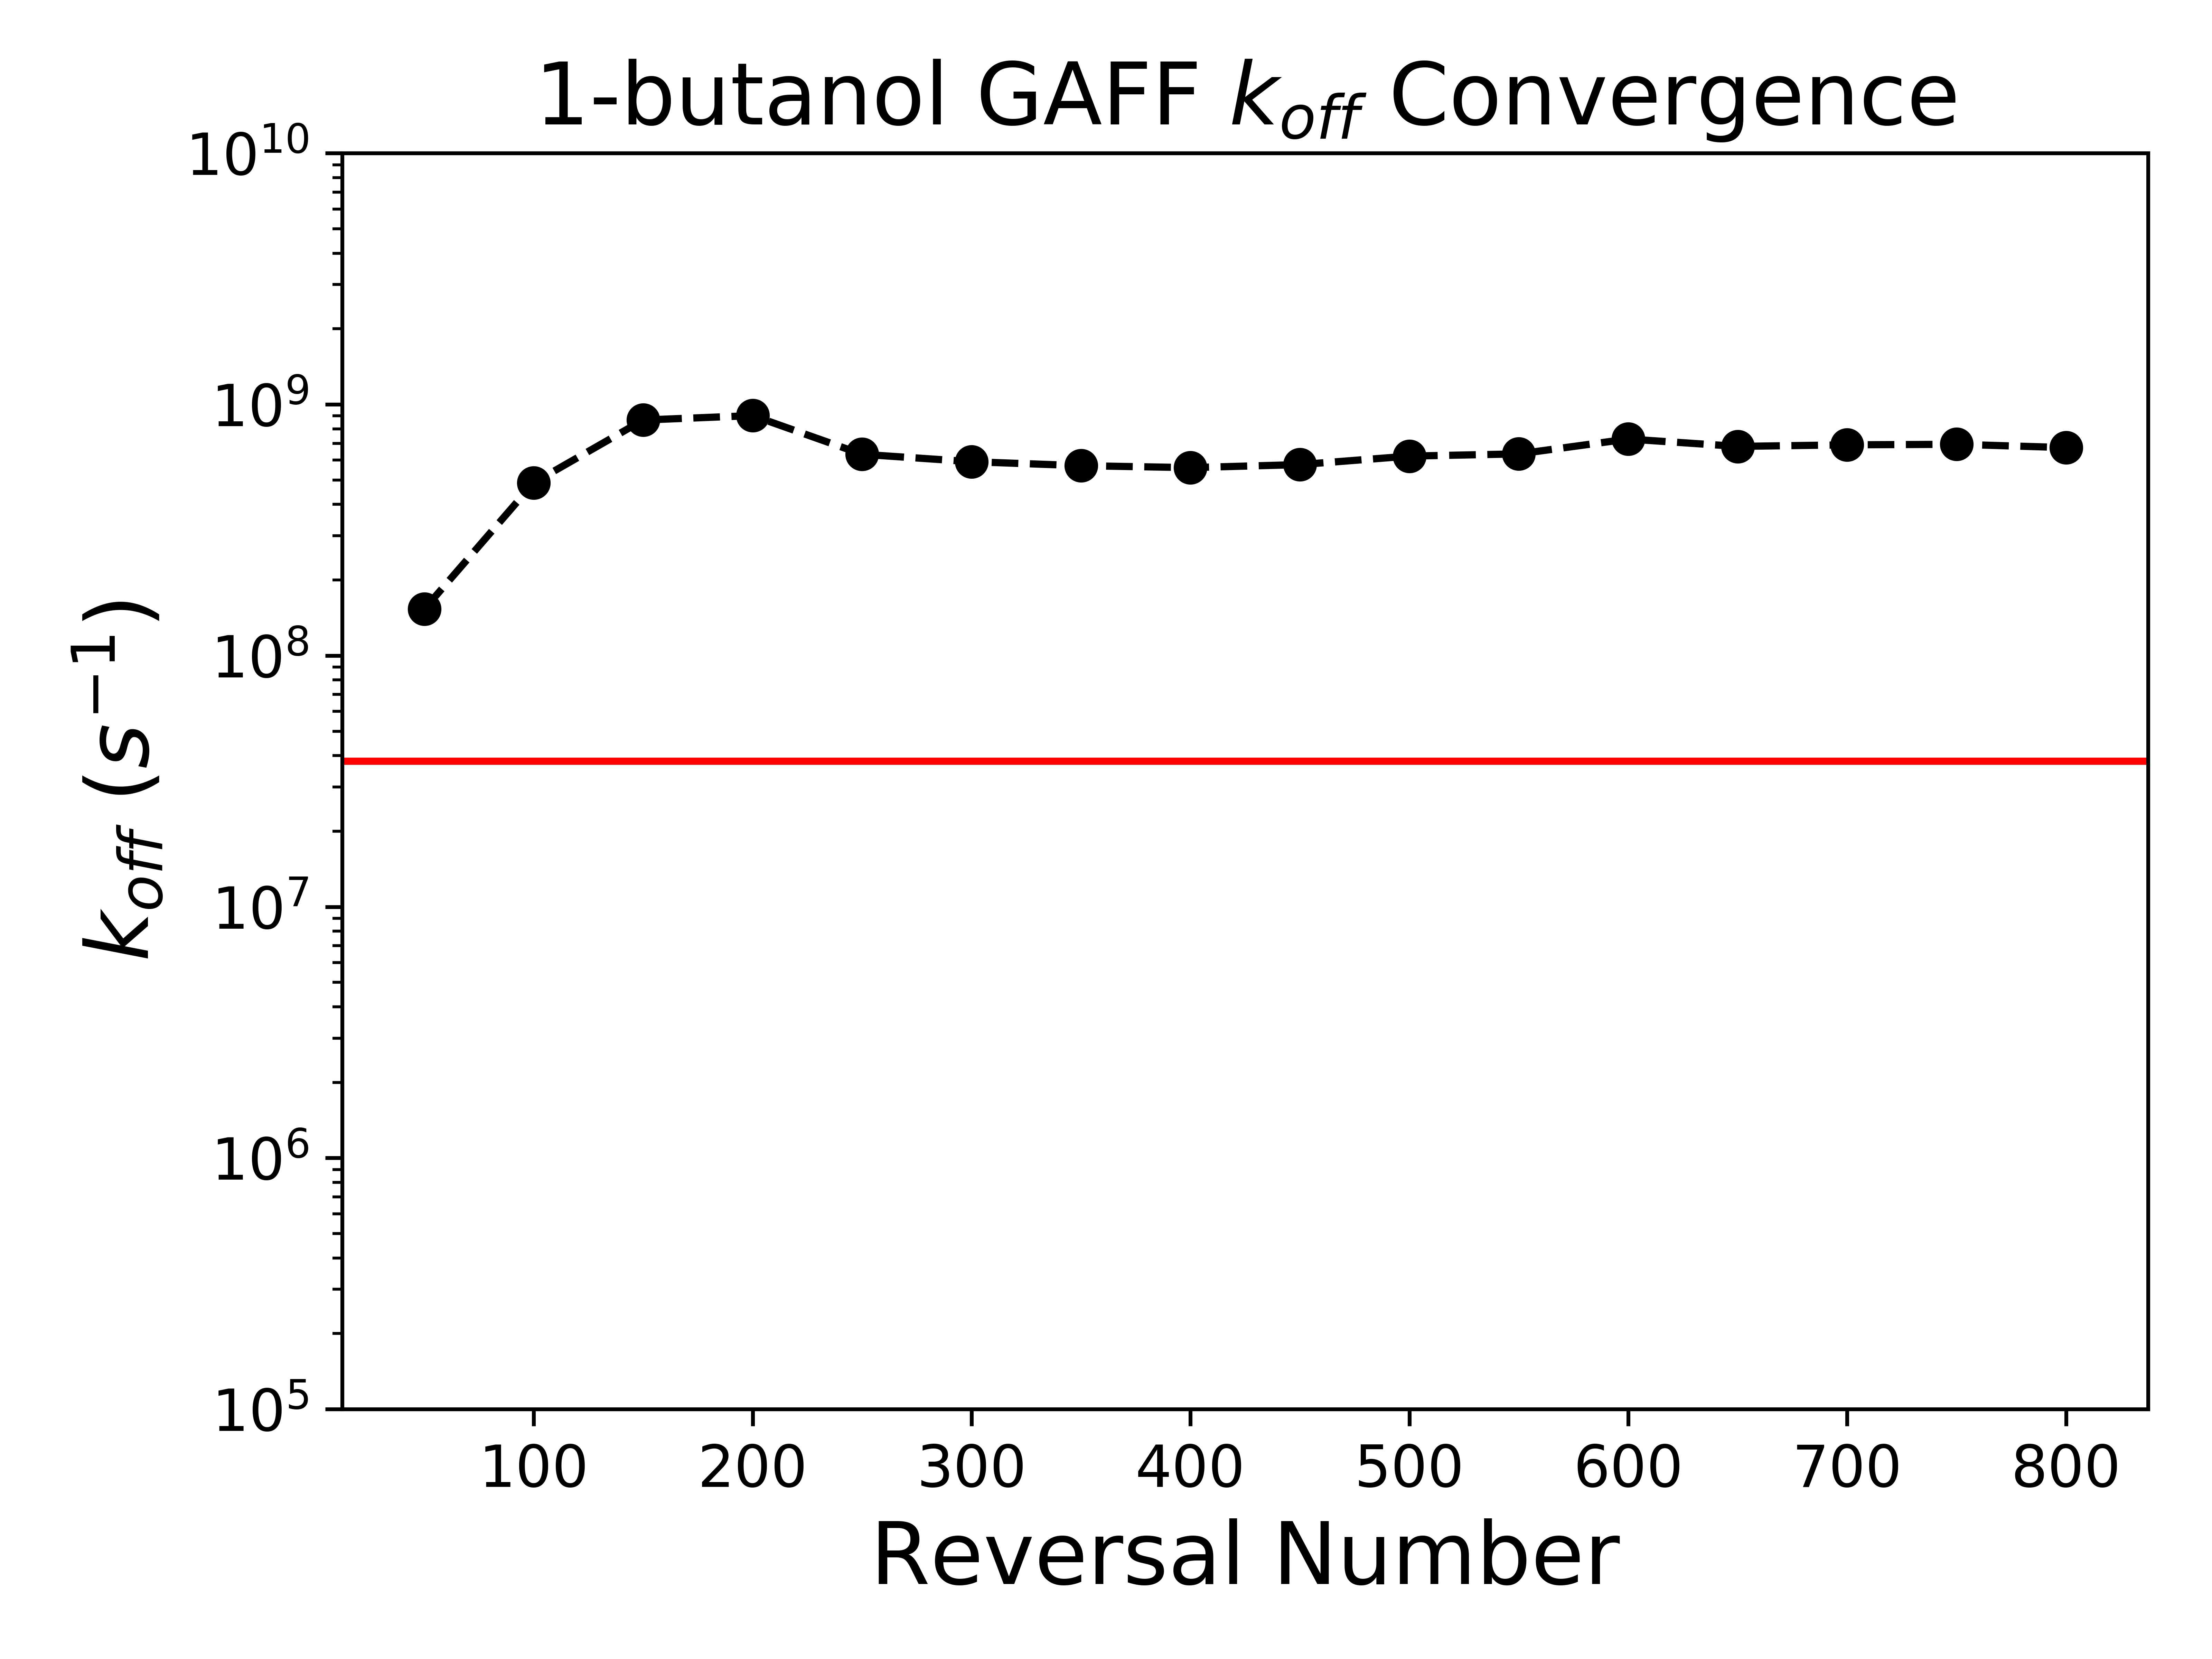
\includegraphics[width=\linewidth]{high_res_images/gaff_rate_conv_images/1-butanol_gaff_off_conv.png}
	\end{subfigure}%
	\begin{subfigure}{0.3\linewidth}
		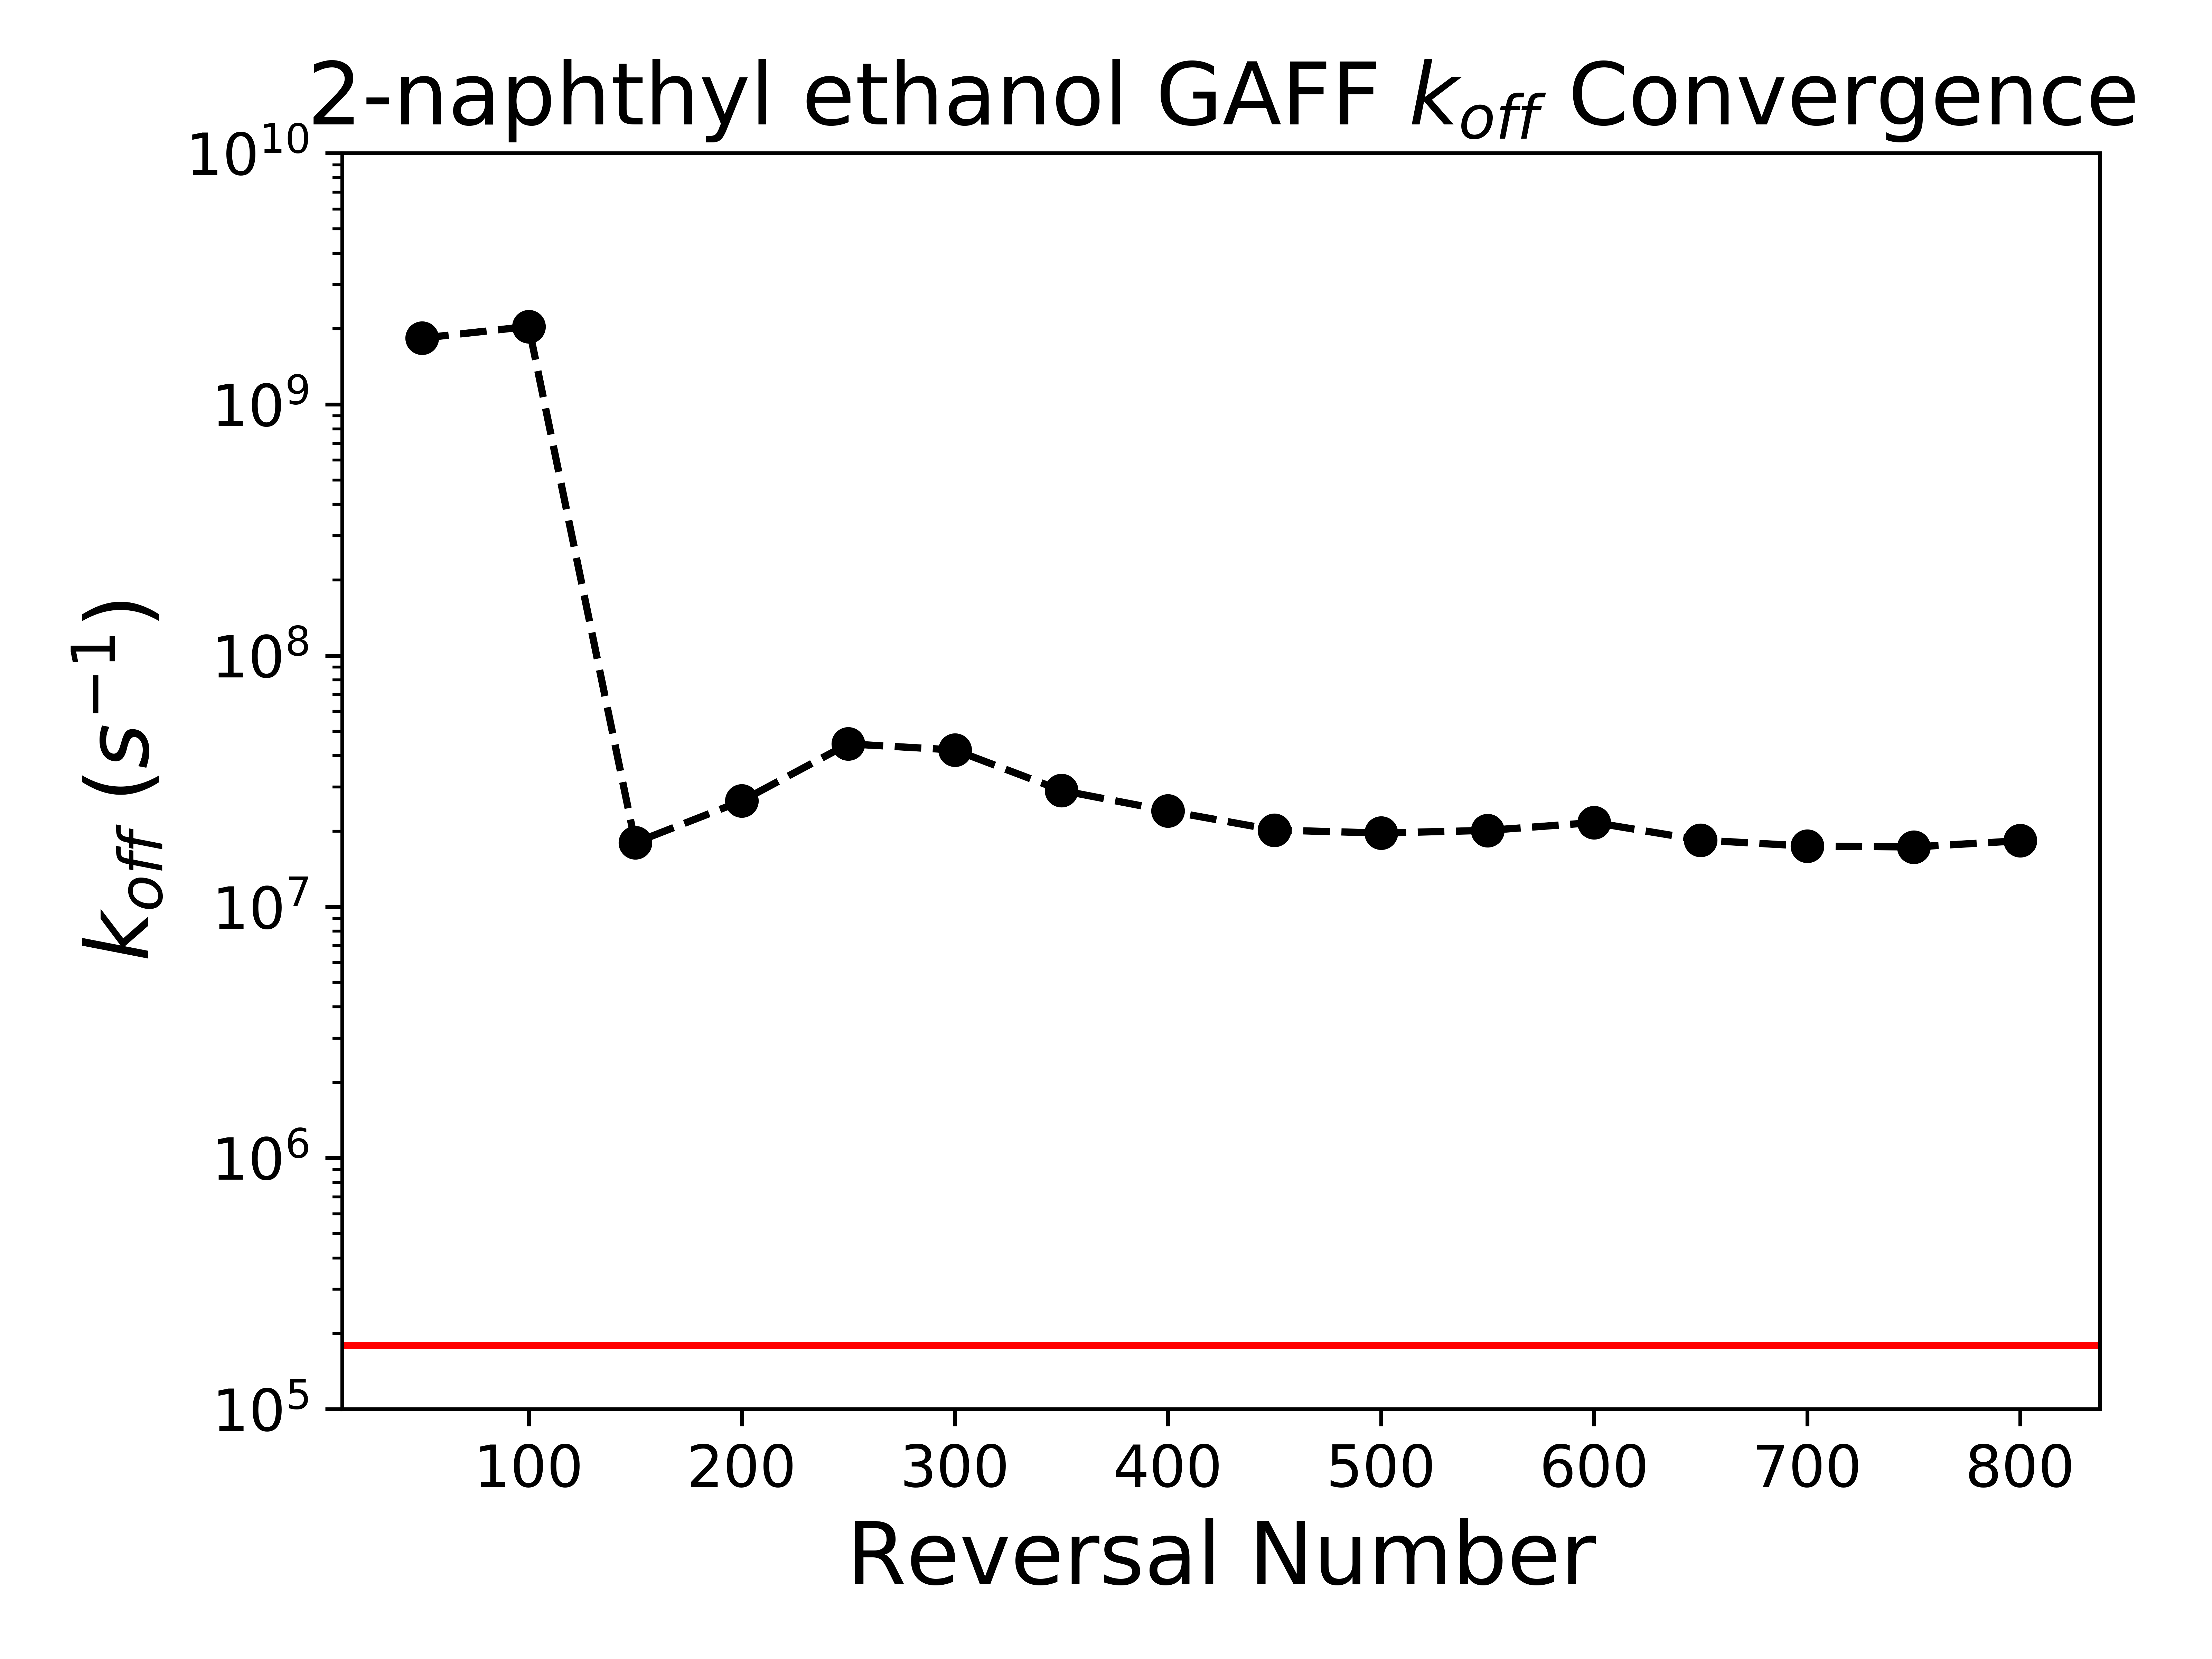
\includegraphics[width=\linewidth]{high_res_images/gaff_rate_conv_images/2-naphthylethanol_gaff_off_conv.png}
	\end{subfigure}%
	\begin{subfigure}{0.3\linewidth}
		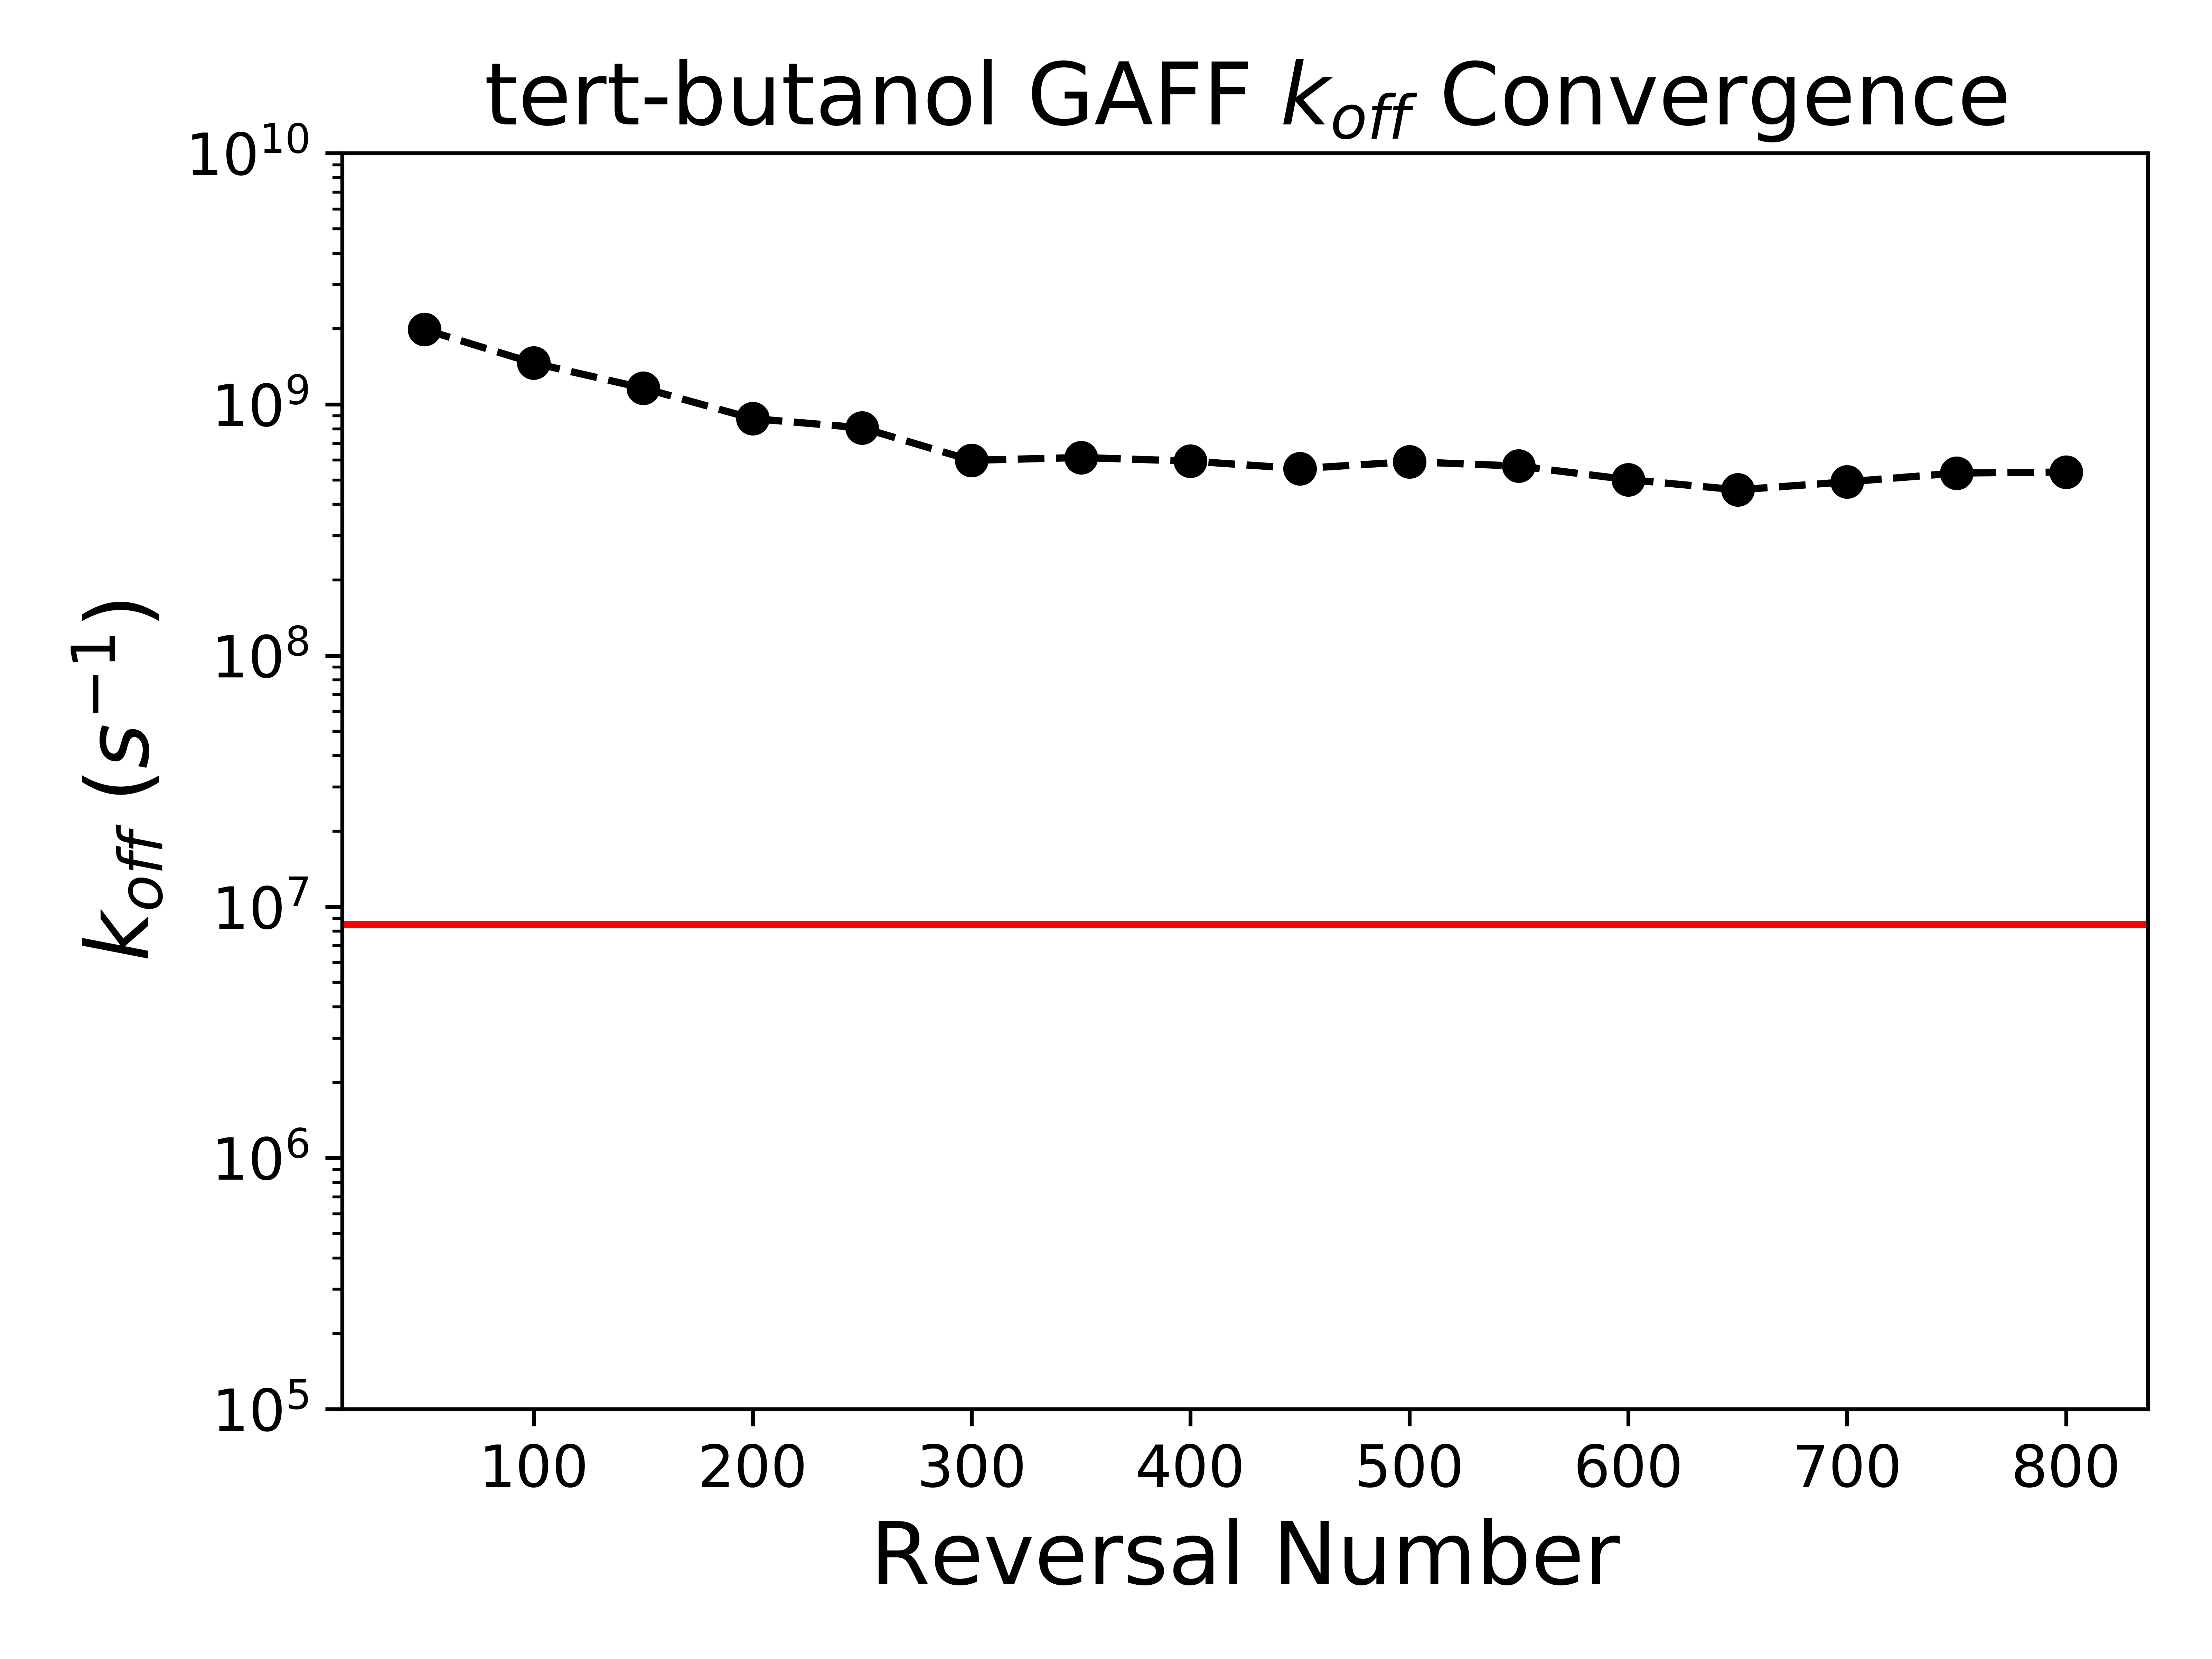
\includegraphics[width=\linewidth]{high_res_images/gaff_rate_conv_images/tert-butanol_gaff_off_conv.png}
	\end{subfigure}
	\begin{subfigure}{0.3\linewidth}
		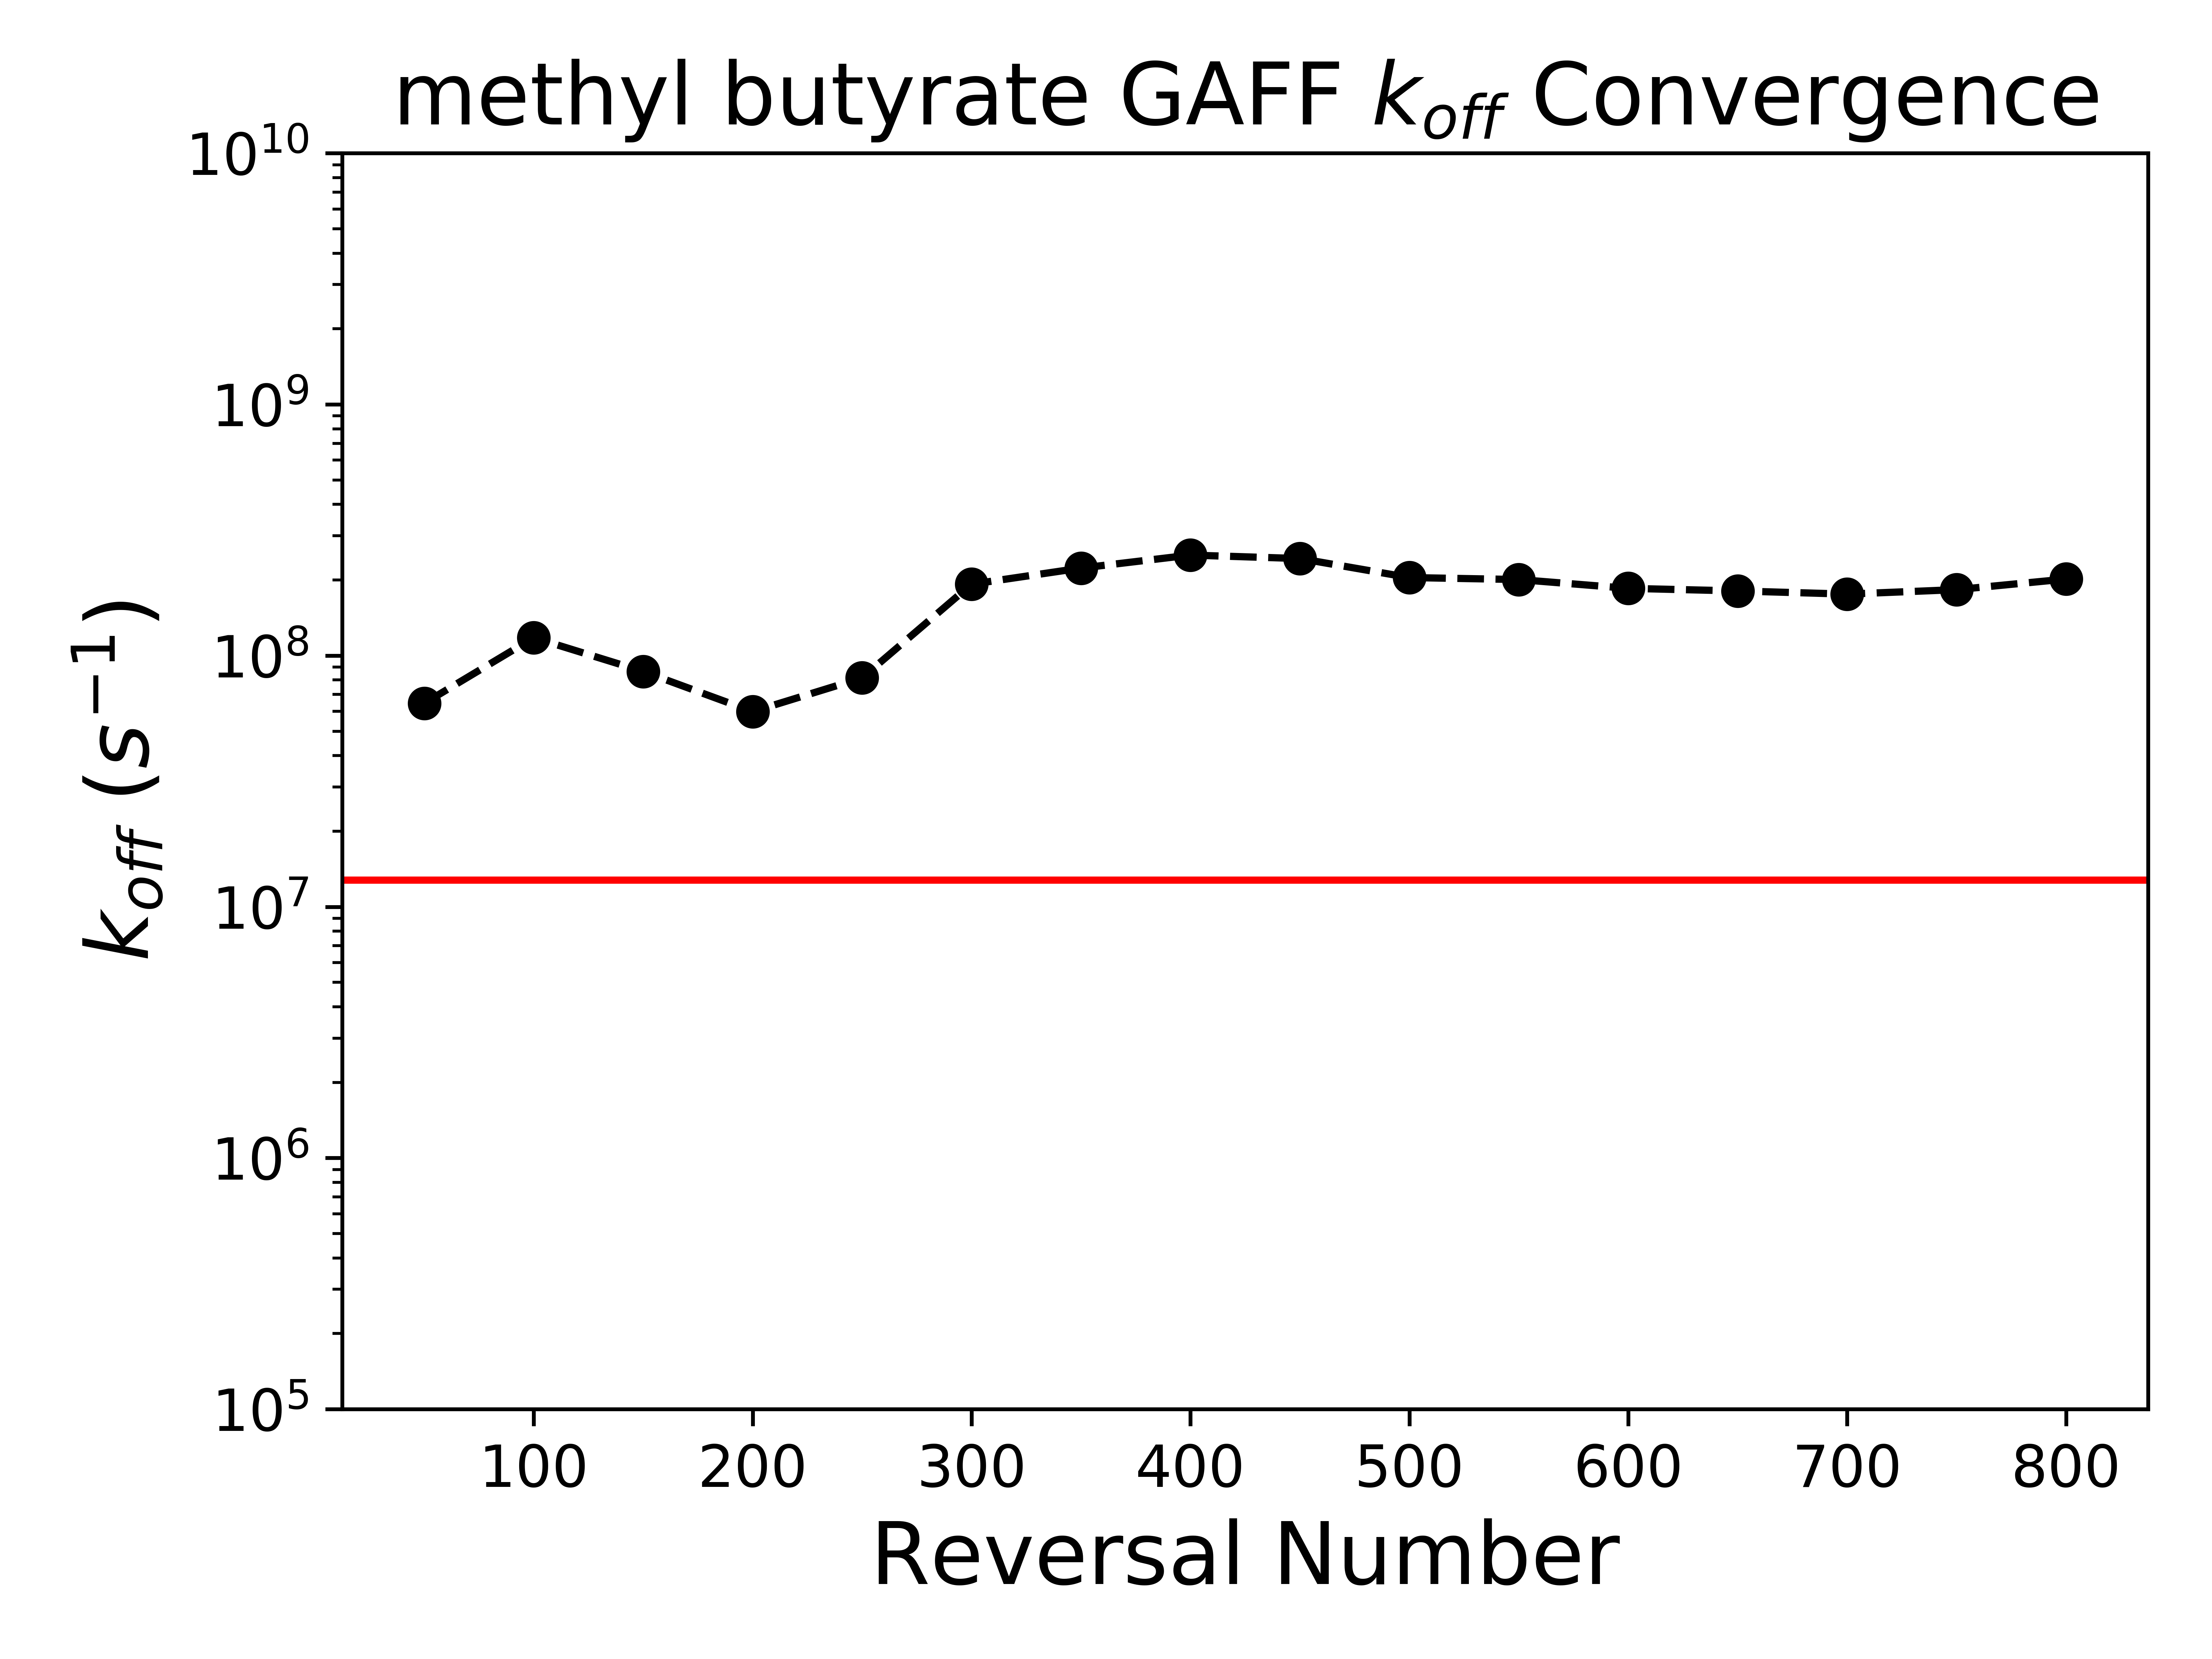
\includegraphics[width=\linewidth]{high_res_images/gaff_rate_conv_images/methylbutyrate_gaff_off_conv.png}
	\end{subfigure}
	\begin{subfigure}{0.3\linewidth}
		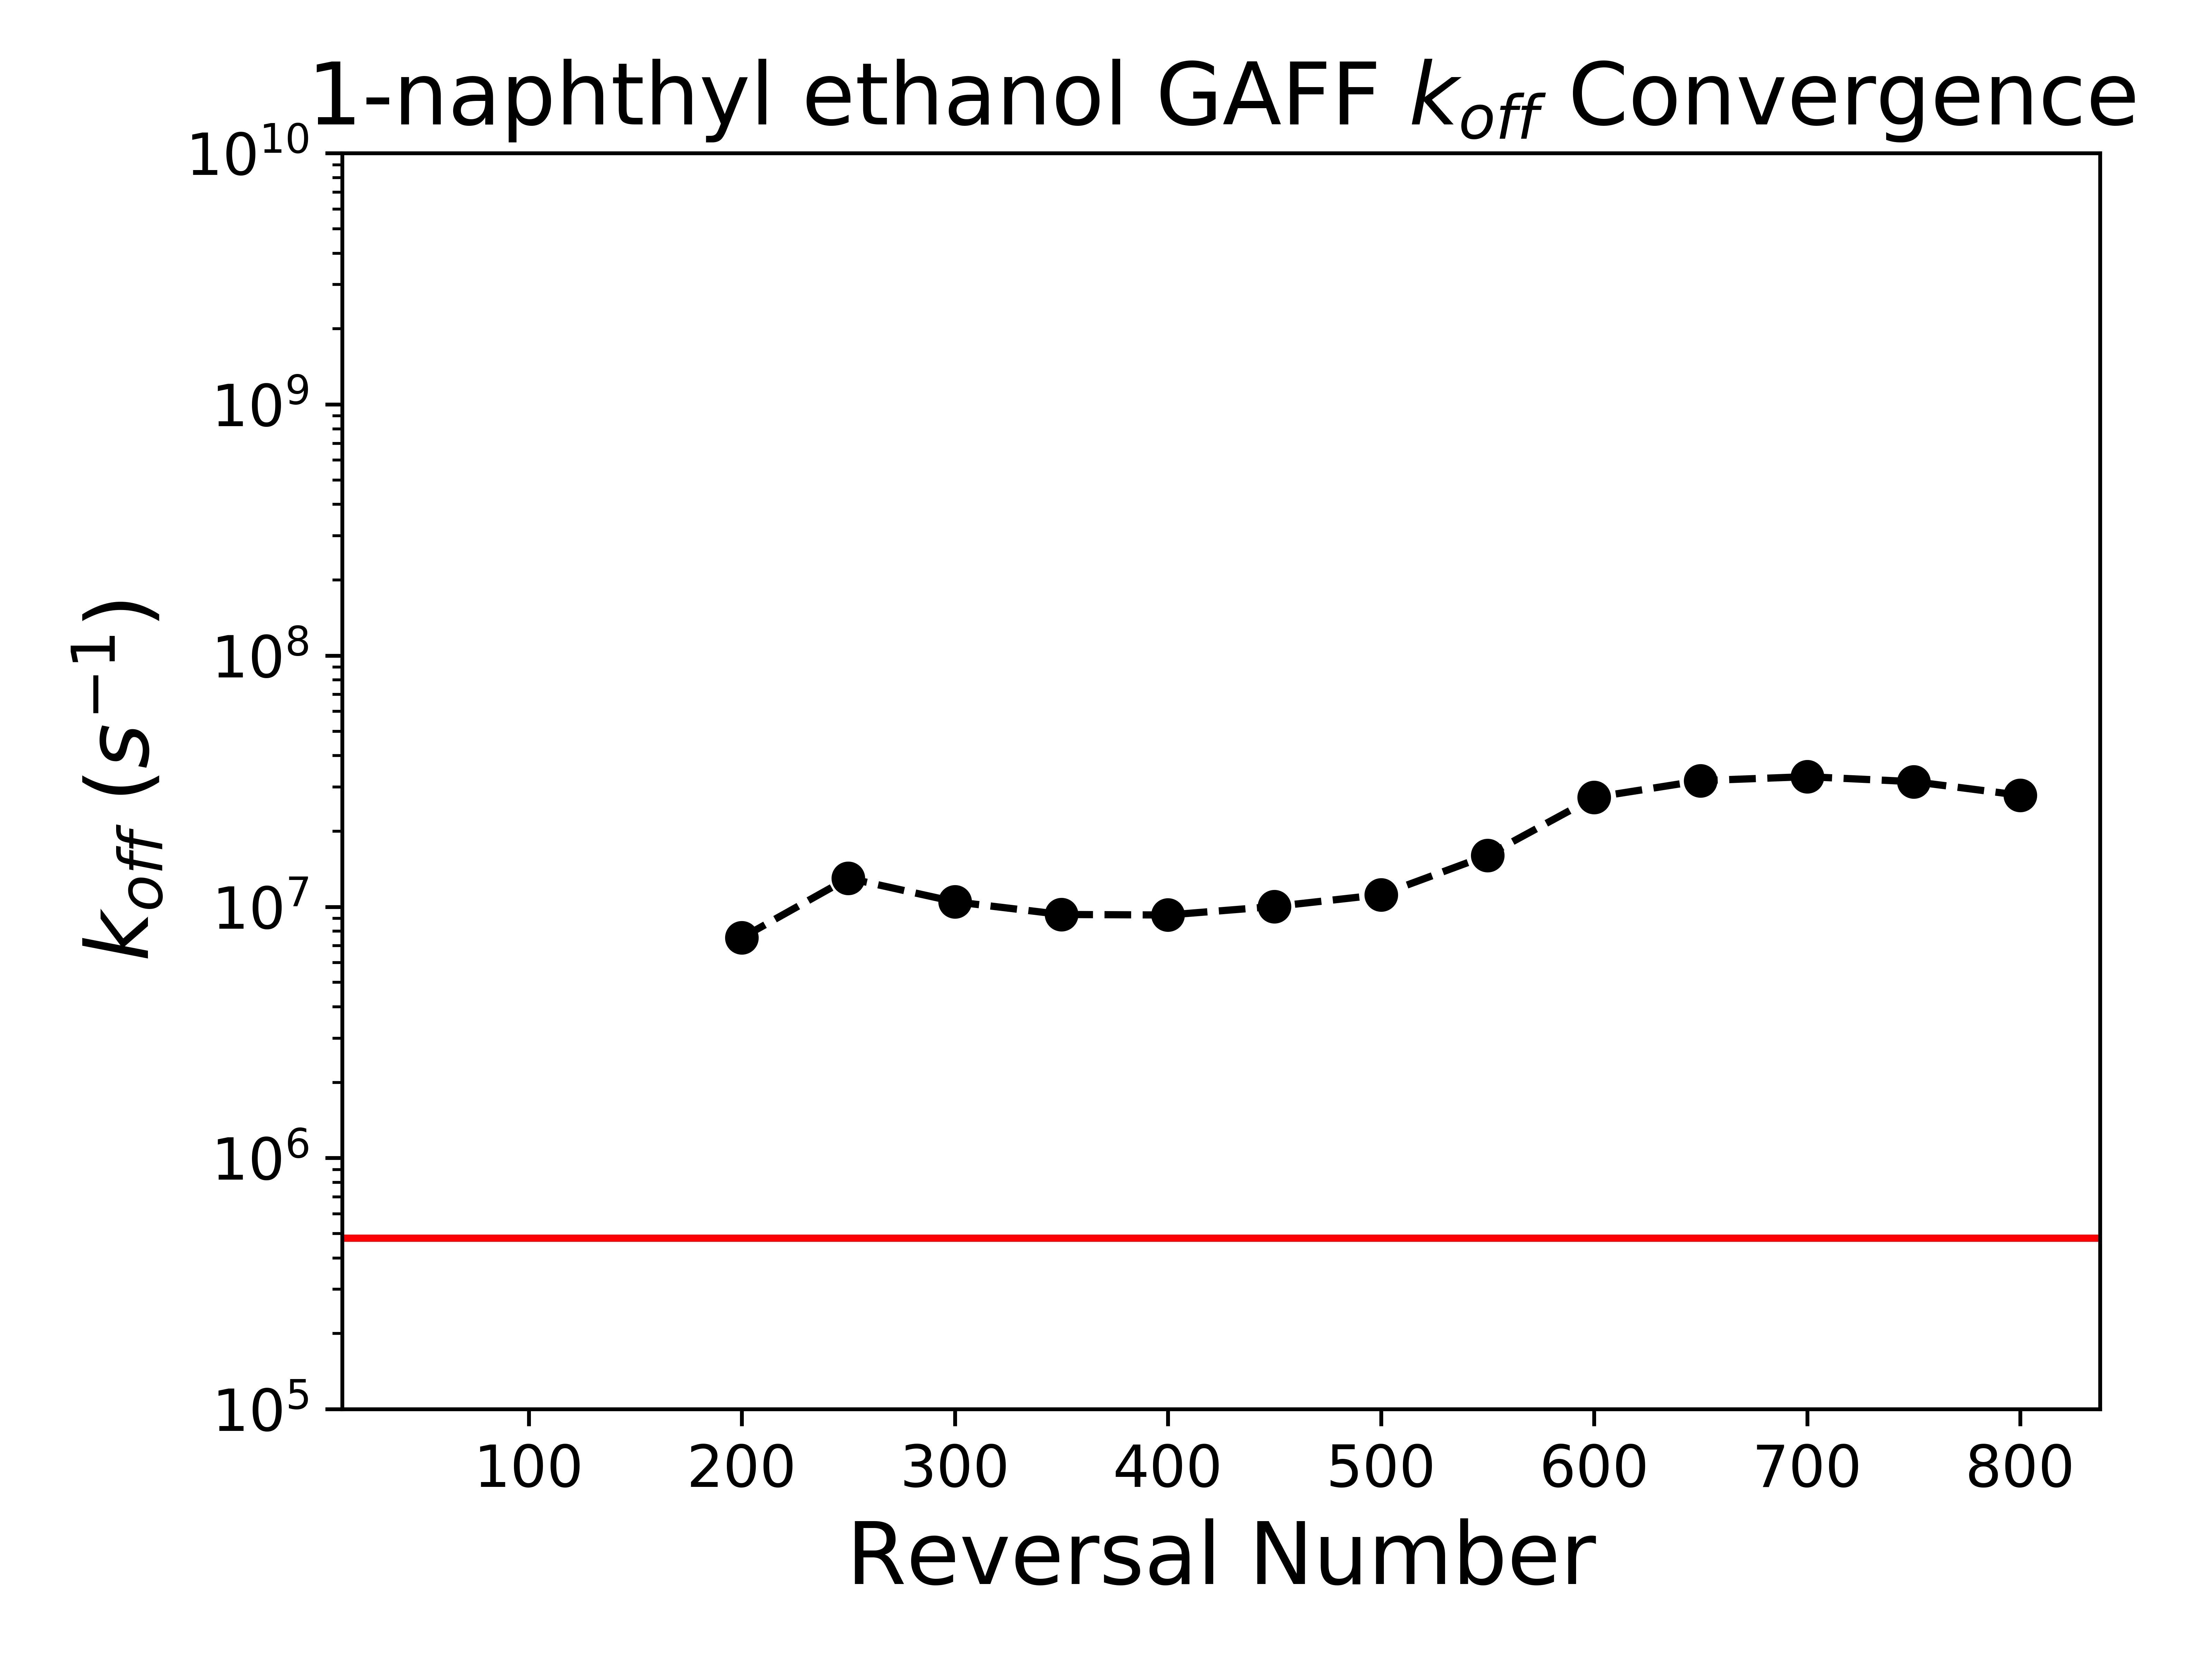
\includegraphics[width=\linewidth]{high_res_images/gaff_rate_conv_images/1-naphthylethanol_gaff_off_conv.png}
	\end{subfigure}
	\begin{subfigure}{0.3\linewidth}
		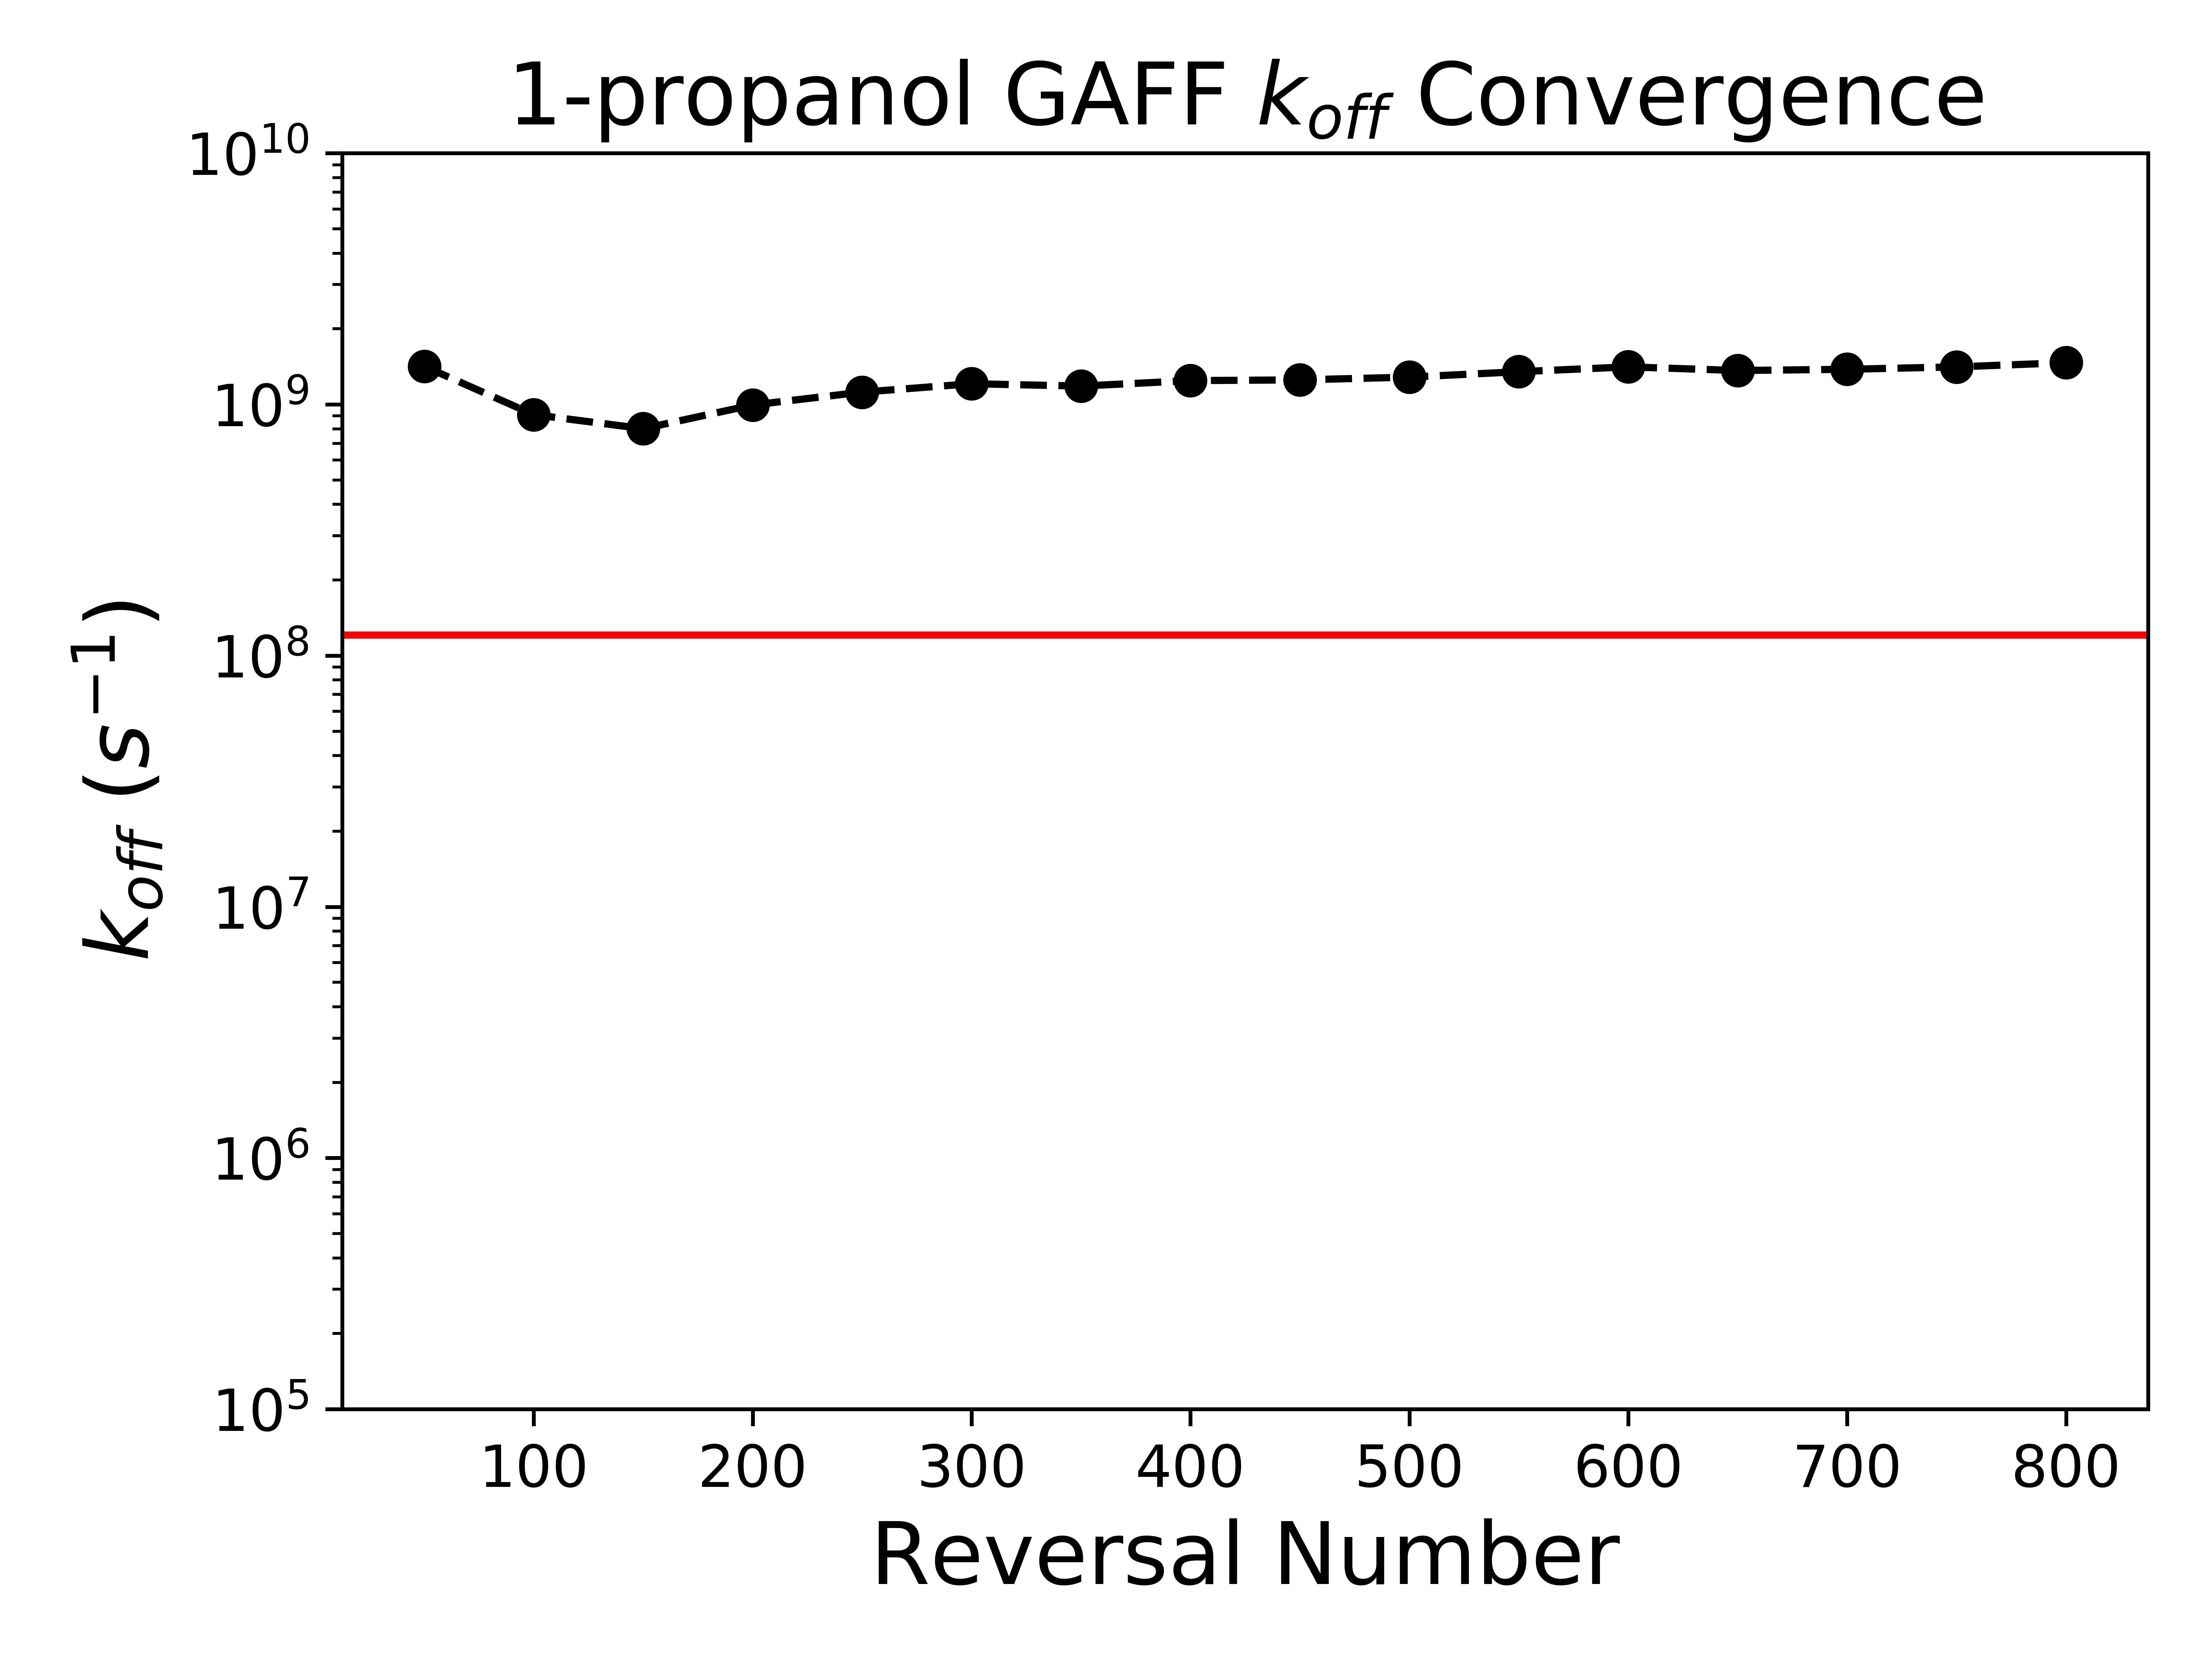
\includegraphics[width=\linewidth]{high_res_images/gaff_rate_conv_images/1-propanol_gaff_off_conv.png}
	\end{subfigure}
	\begin{subfigure}{0.3\linewidth}
		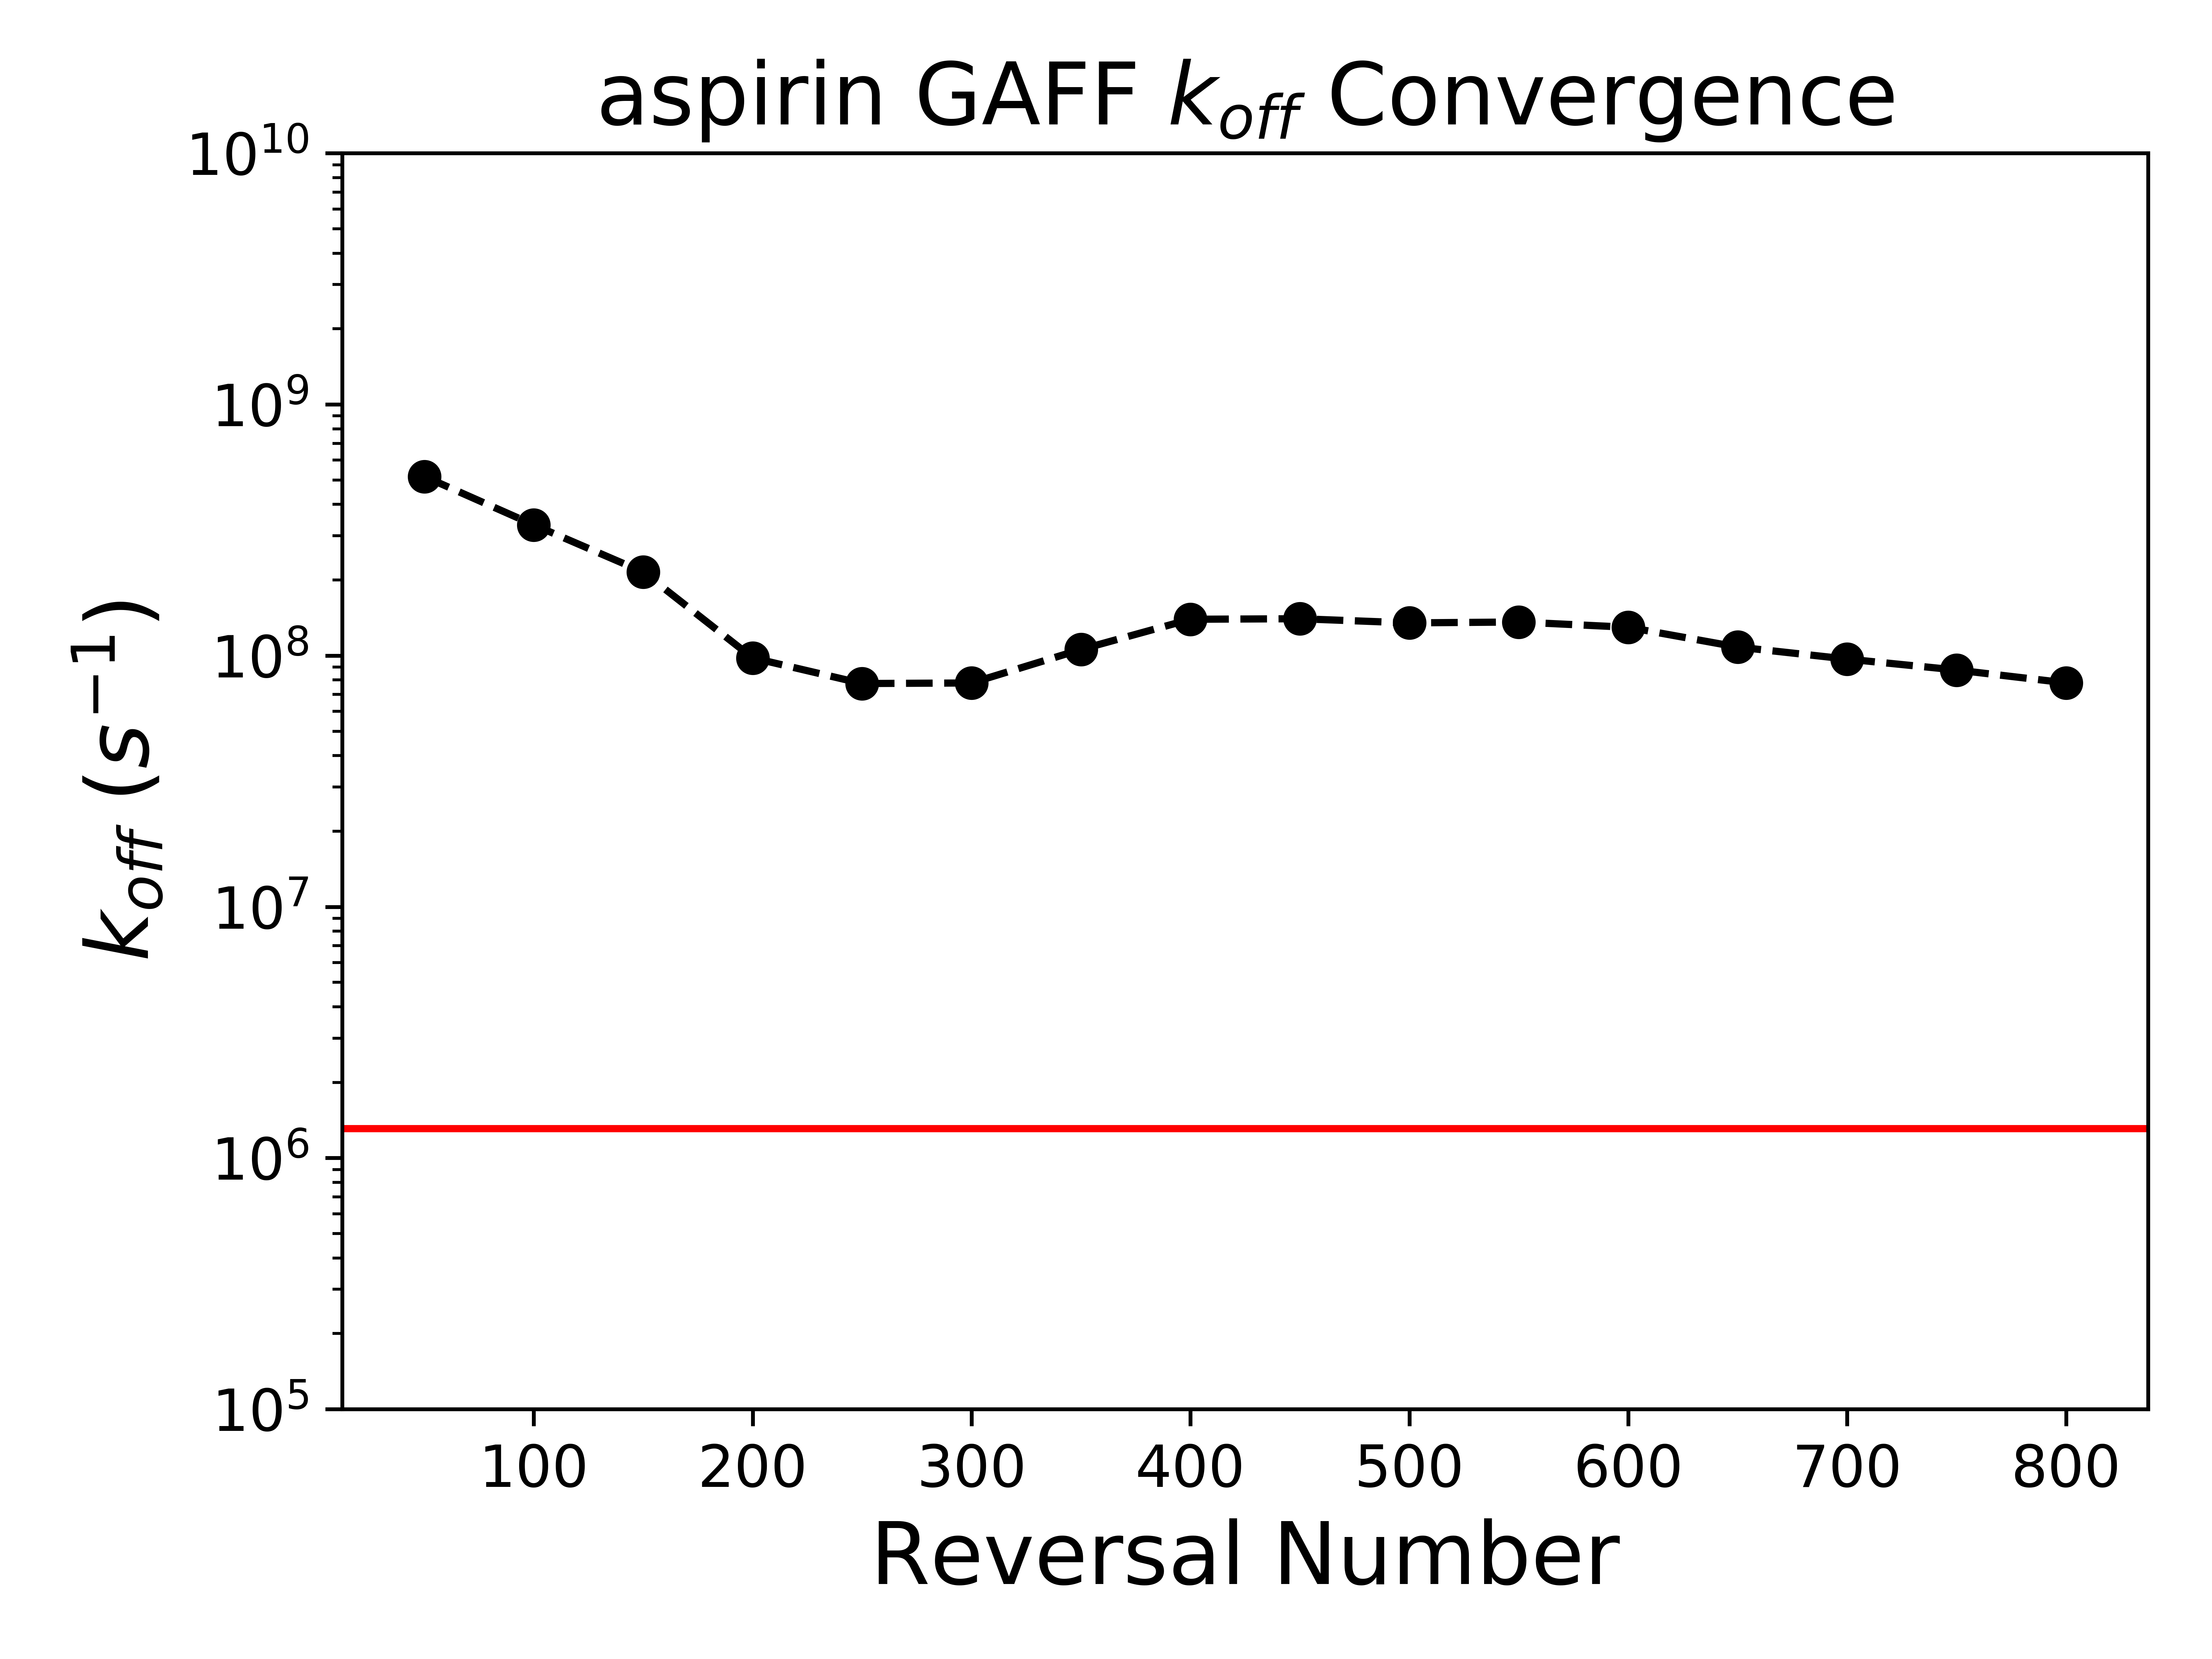
\includegraphics[width=\linewidth]{high_res_images/gaff_rate_conv_images/aspirin_gaff_off_conv.png}
	\end{subfigure}
	\caption{Convergence of off rates as a function of the number of reversals included using the GAFF forcefield}
\end{figure}
%\begin{figure}
\begin{subfigure}{0.3\linewidth}
	\centering
	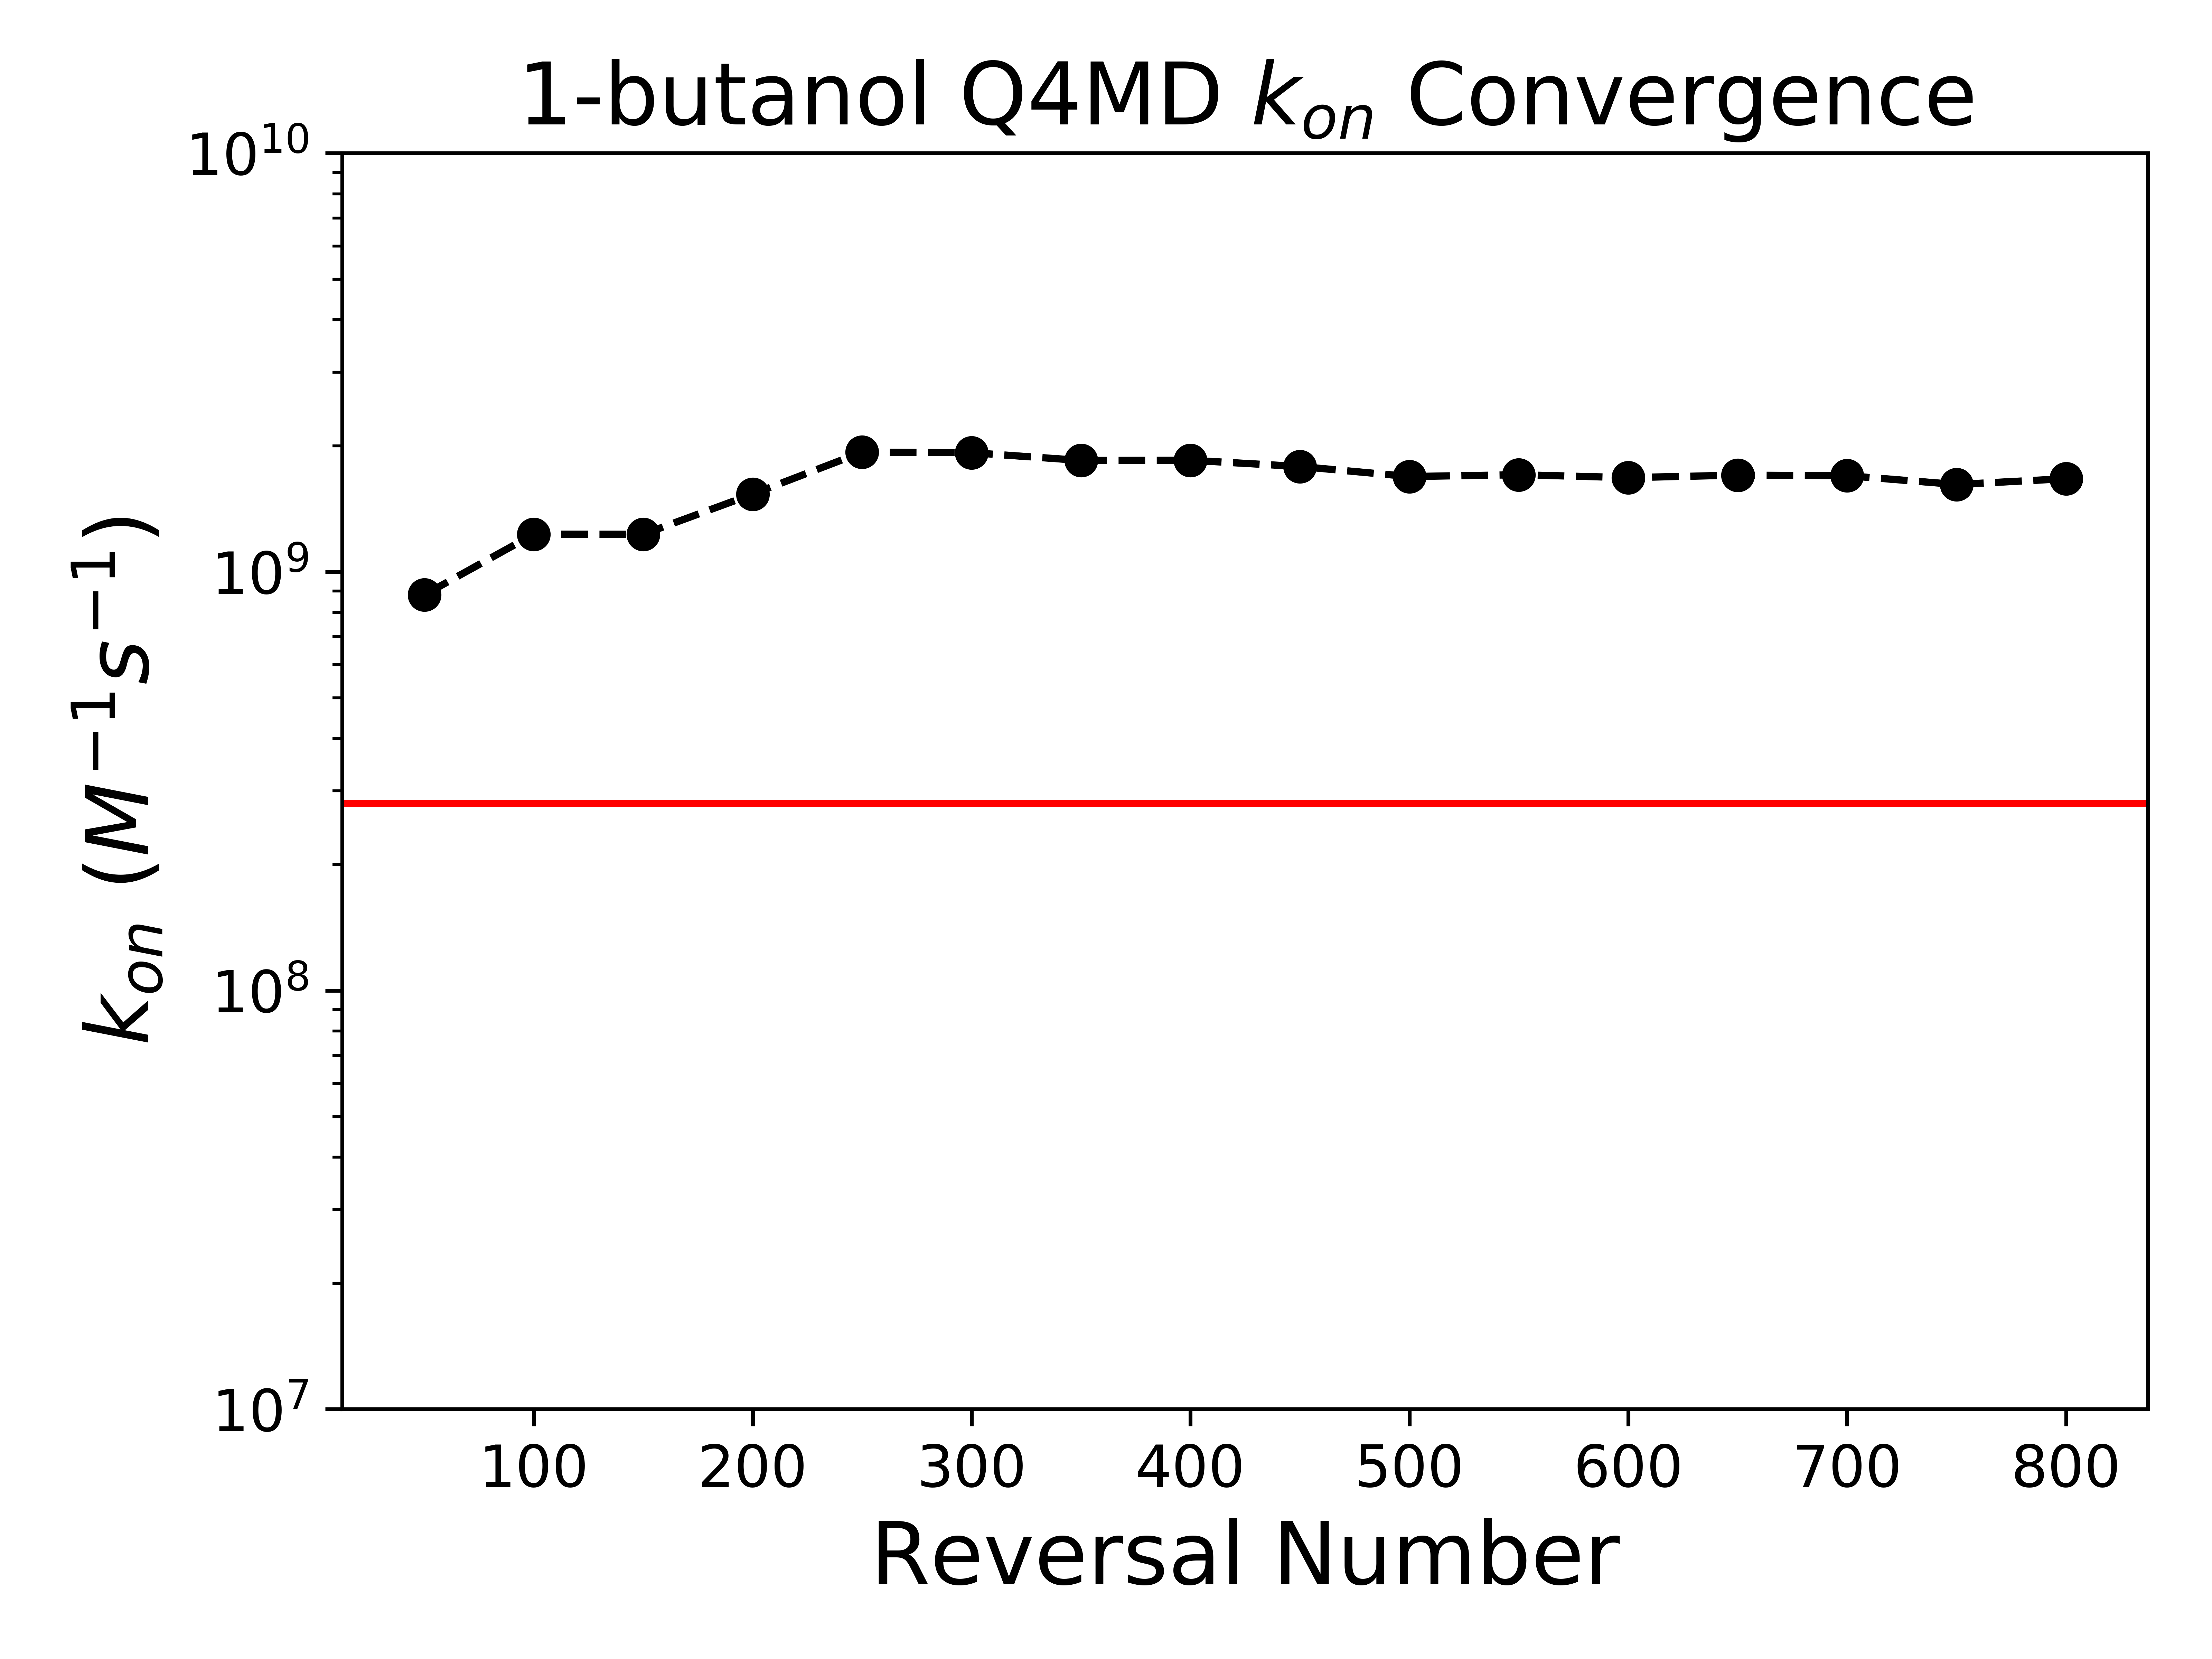
\includegraphics[width=\linewidth]{high_res_images/q4md_rate_conv_images/1-butanol_q4md_on_conv.png}
	\end{subfigure}%
\begin{subfigure}{0.3\linewidth}
		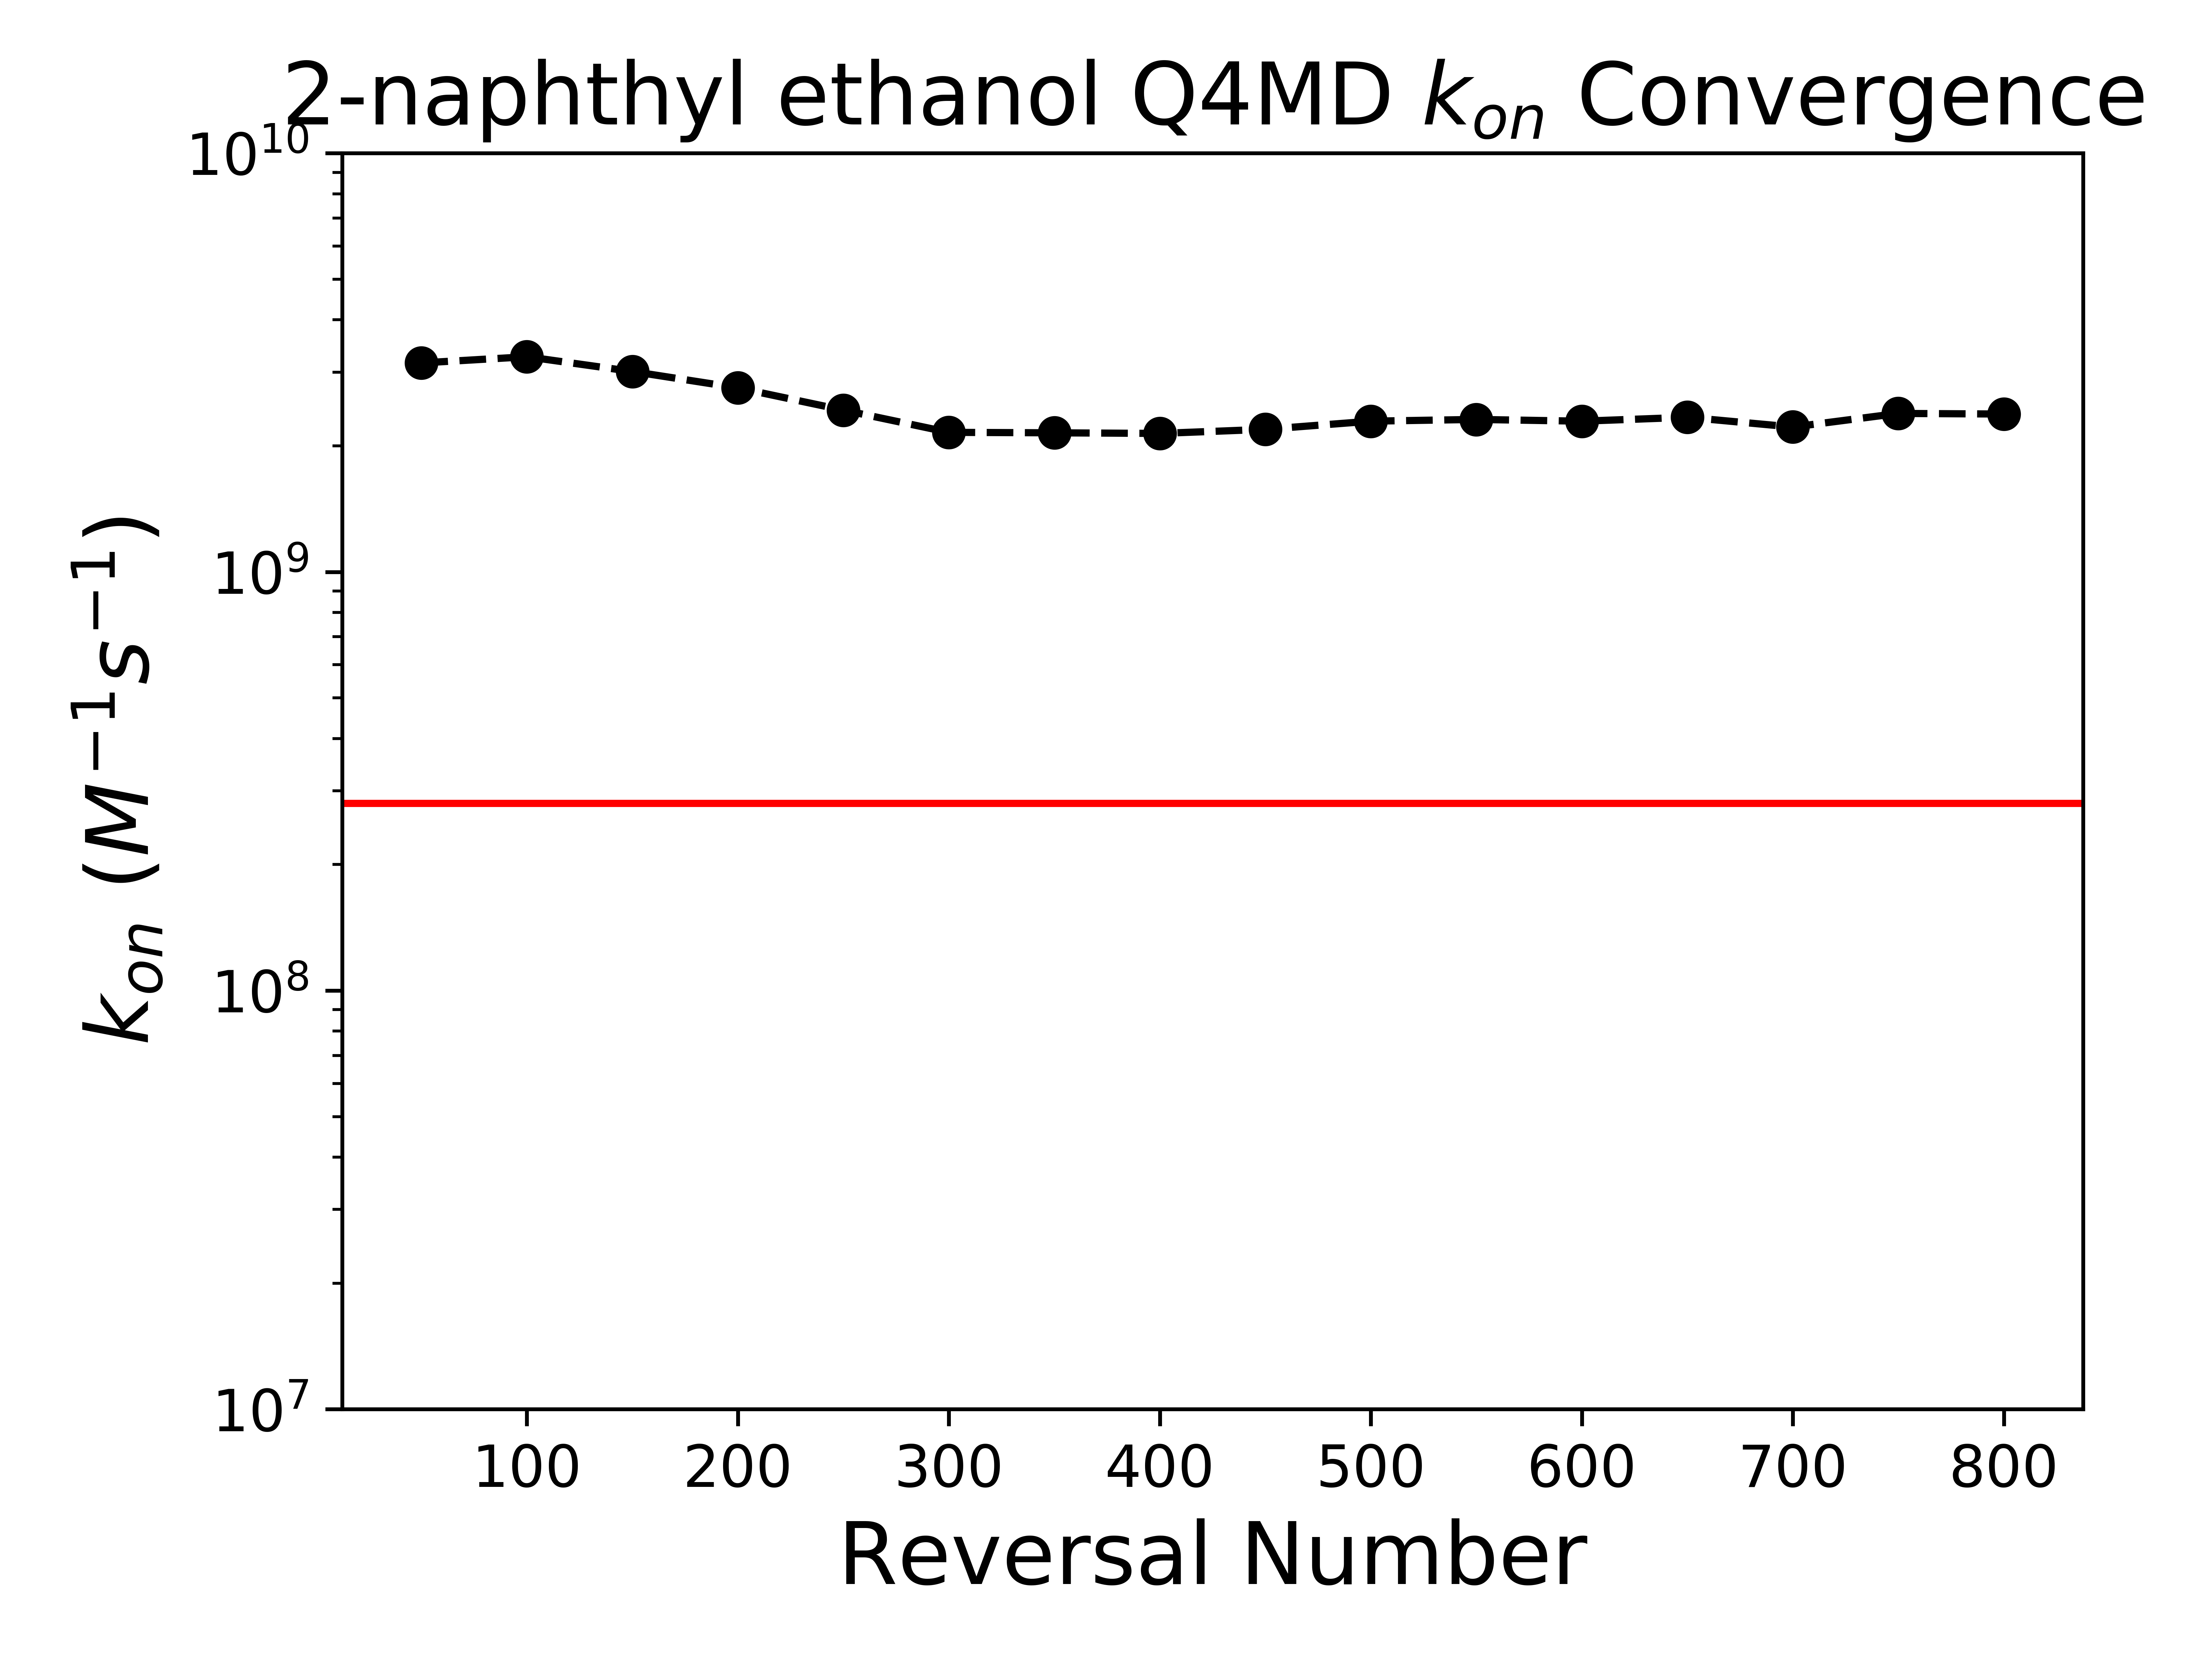
\includegraphics[width=\linewidth]{high_res_images/q4md_rate_conv_images/2-naphthylethanol_q4md_on_conv.png}
\end{subfigure}%
	\begin{subfigure}{0.3\linewidth}
		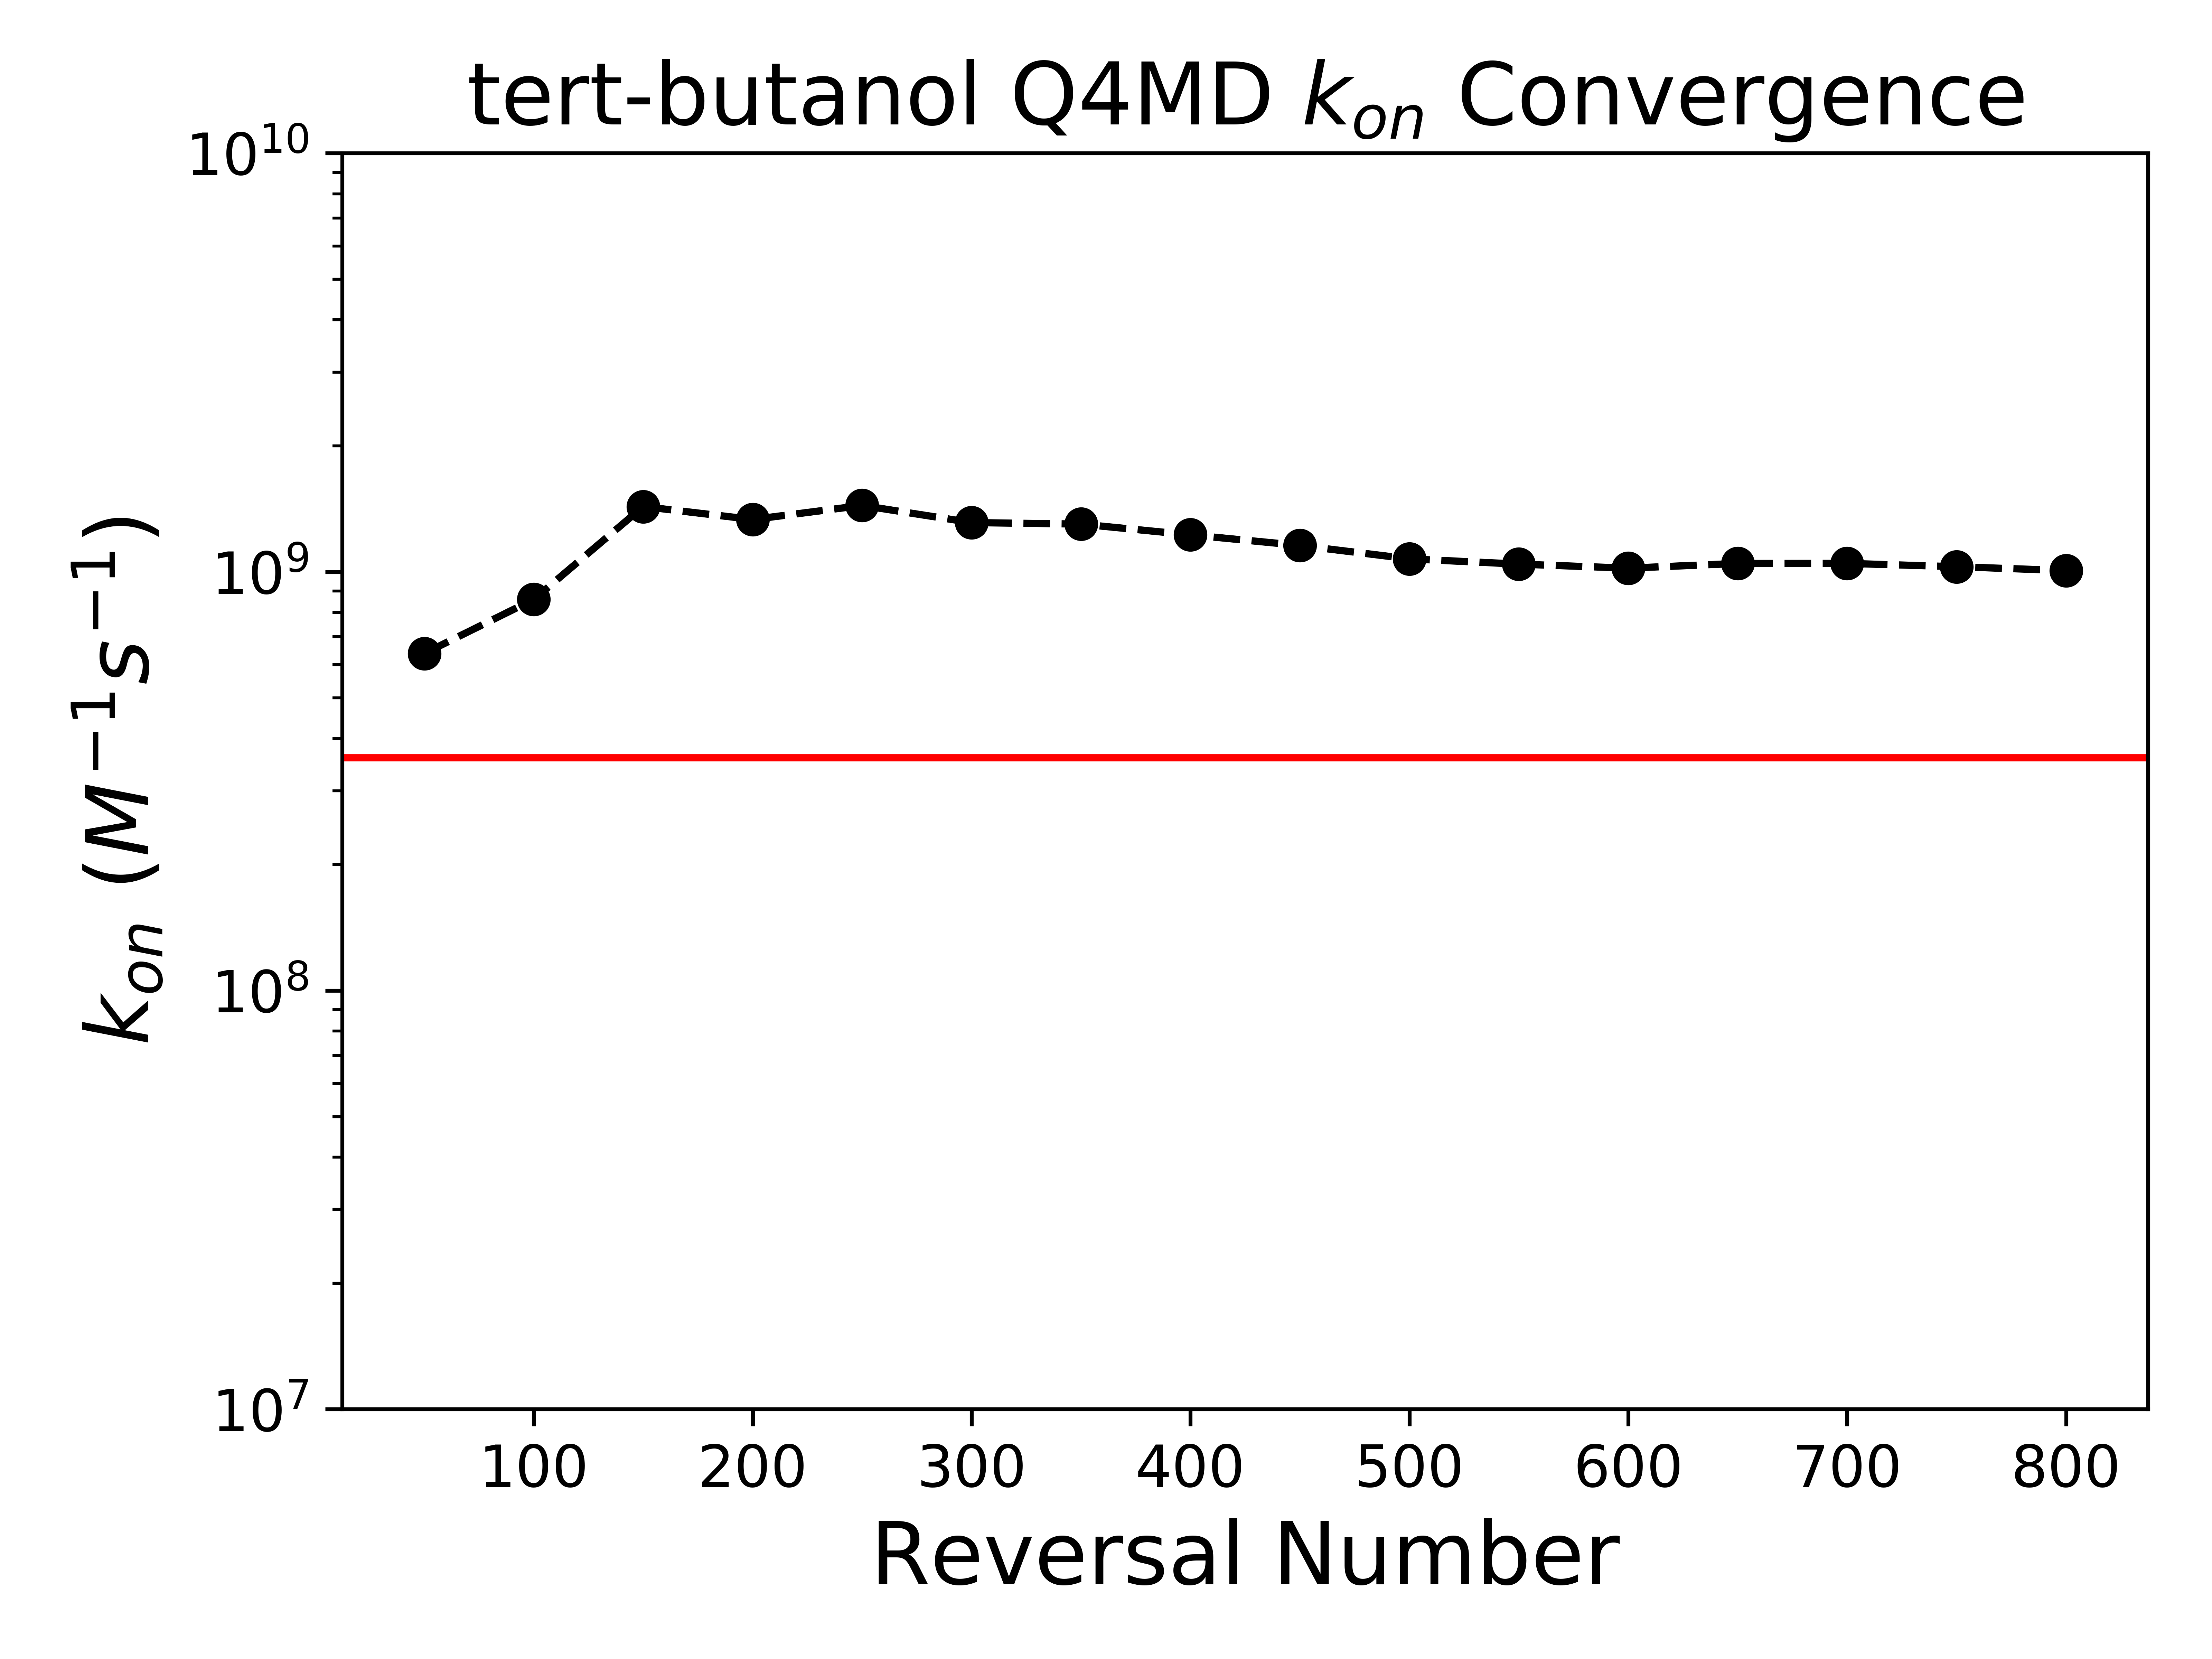
\includegraphics[width=\linewidth]{high_res_images/q4md_rate_conv_images/tert-butanol_q4md_on_conv.png}
	\end{subfigure}
	\begin{subfigure}{0.3\linewidth}
		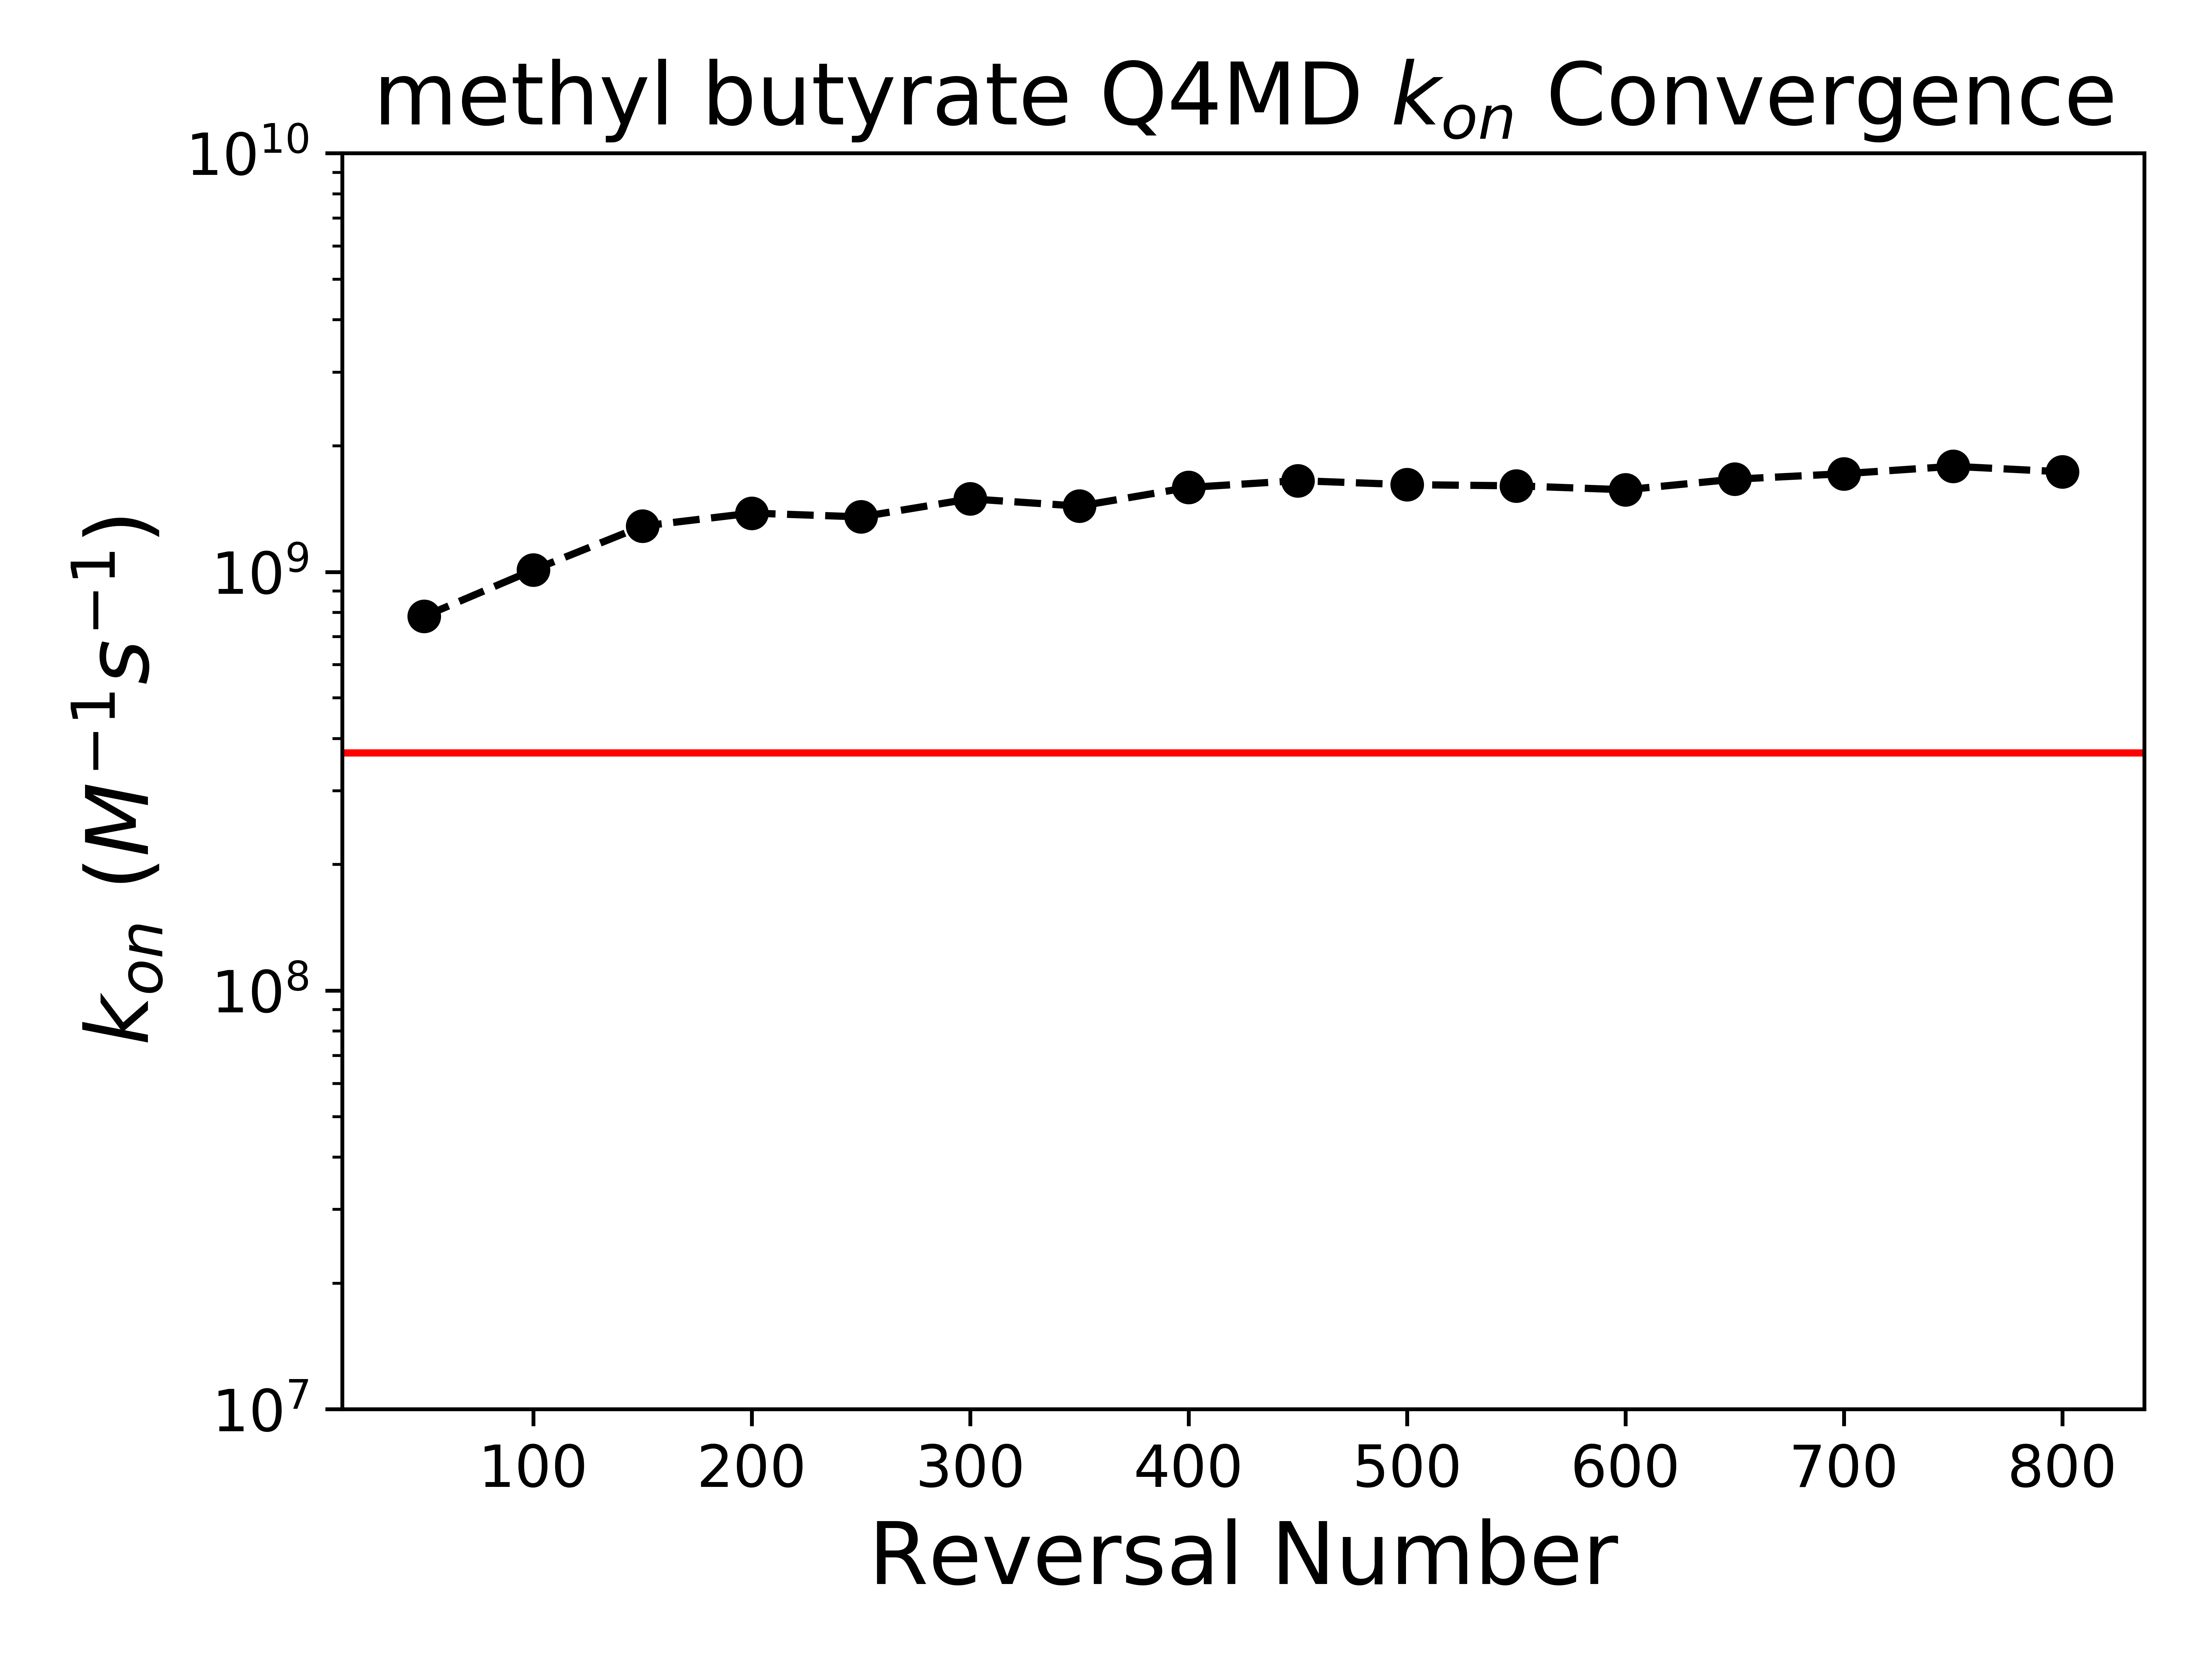
\includegraphics[width=\linewidth]{high_res_images/q4md_rate_conv_images/methylbutyrate_q4md_on_conv.png}
	\end{subfigure}
	\begin{subfigure}{0.3\linewidth}
		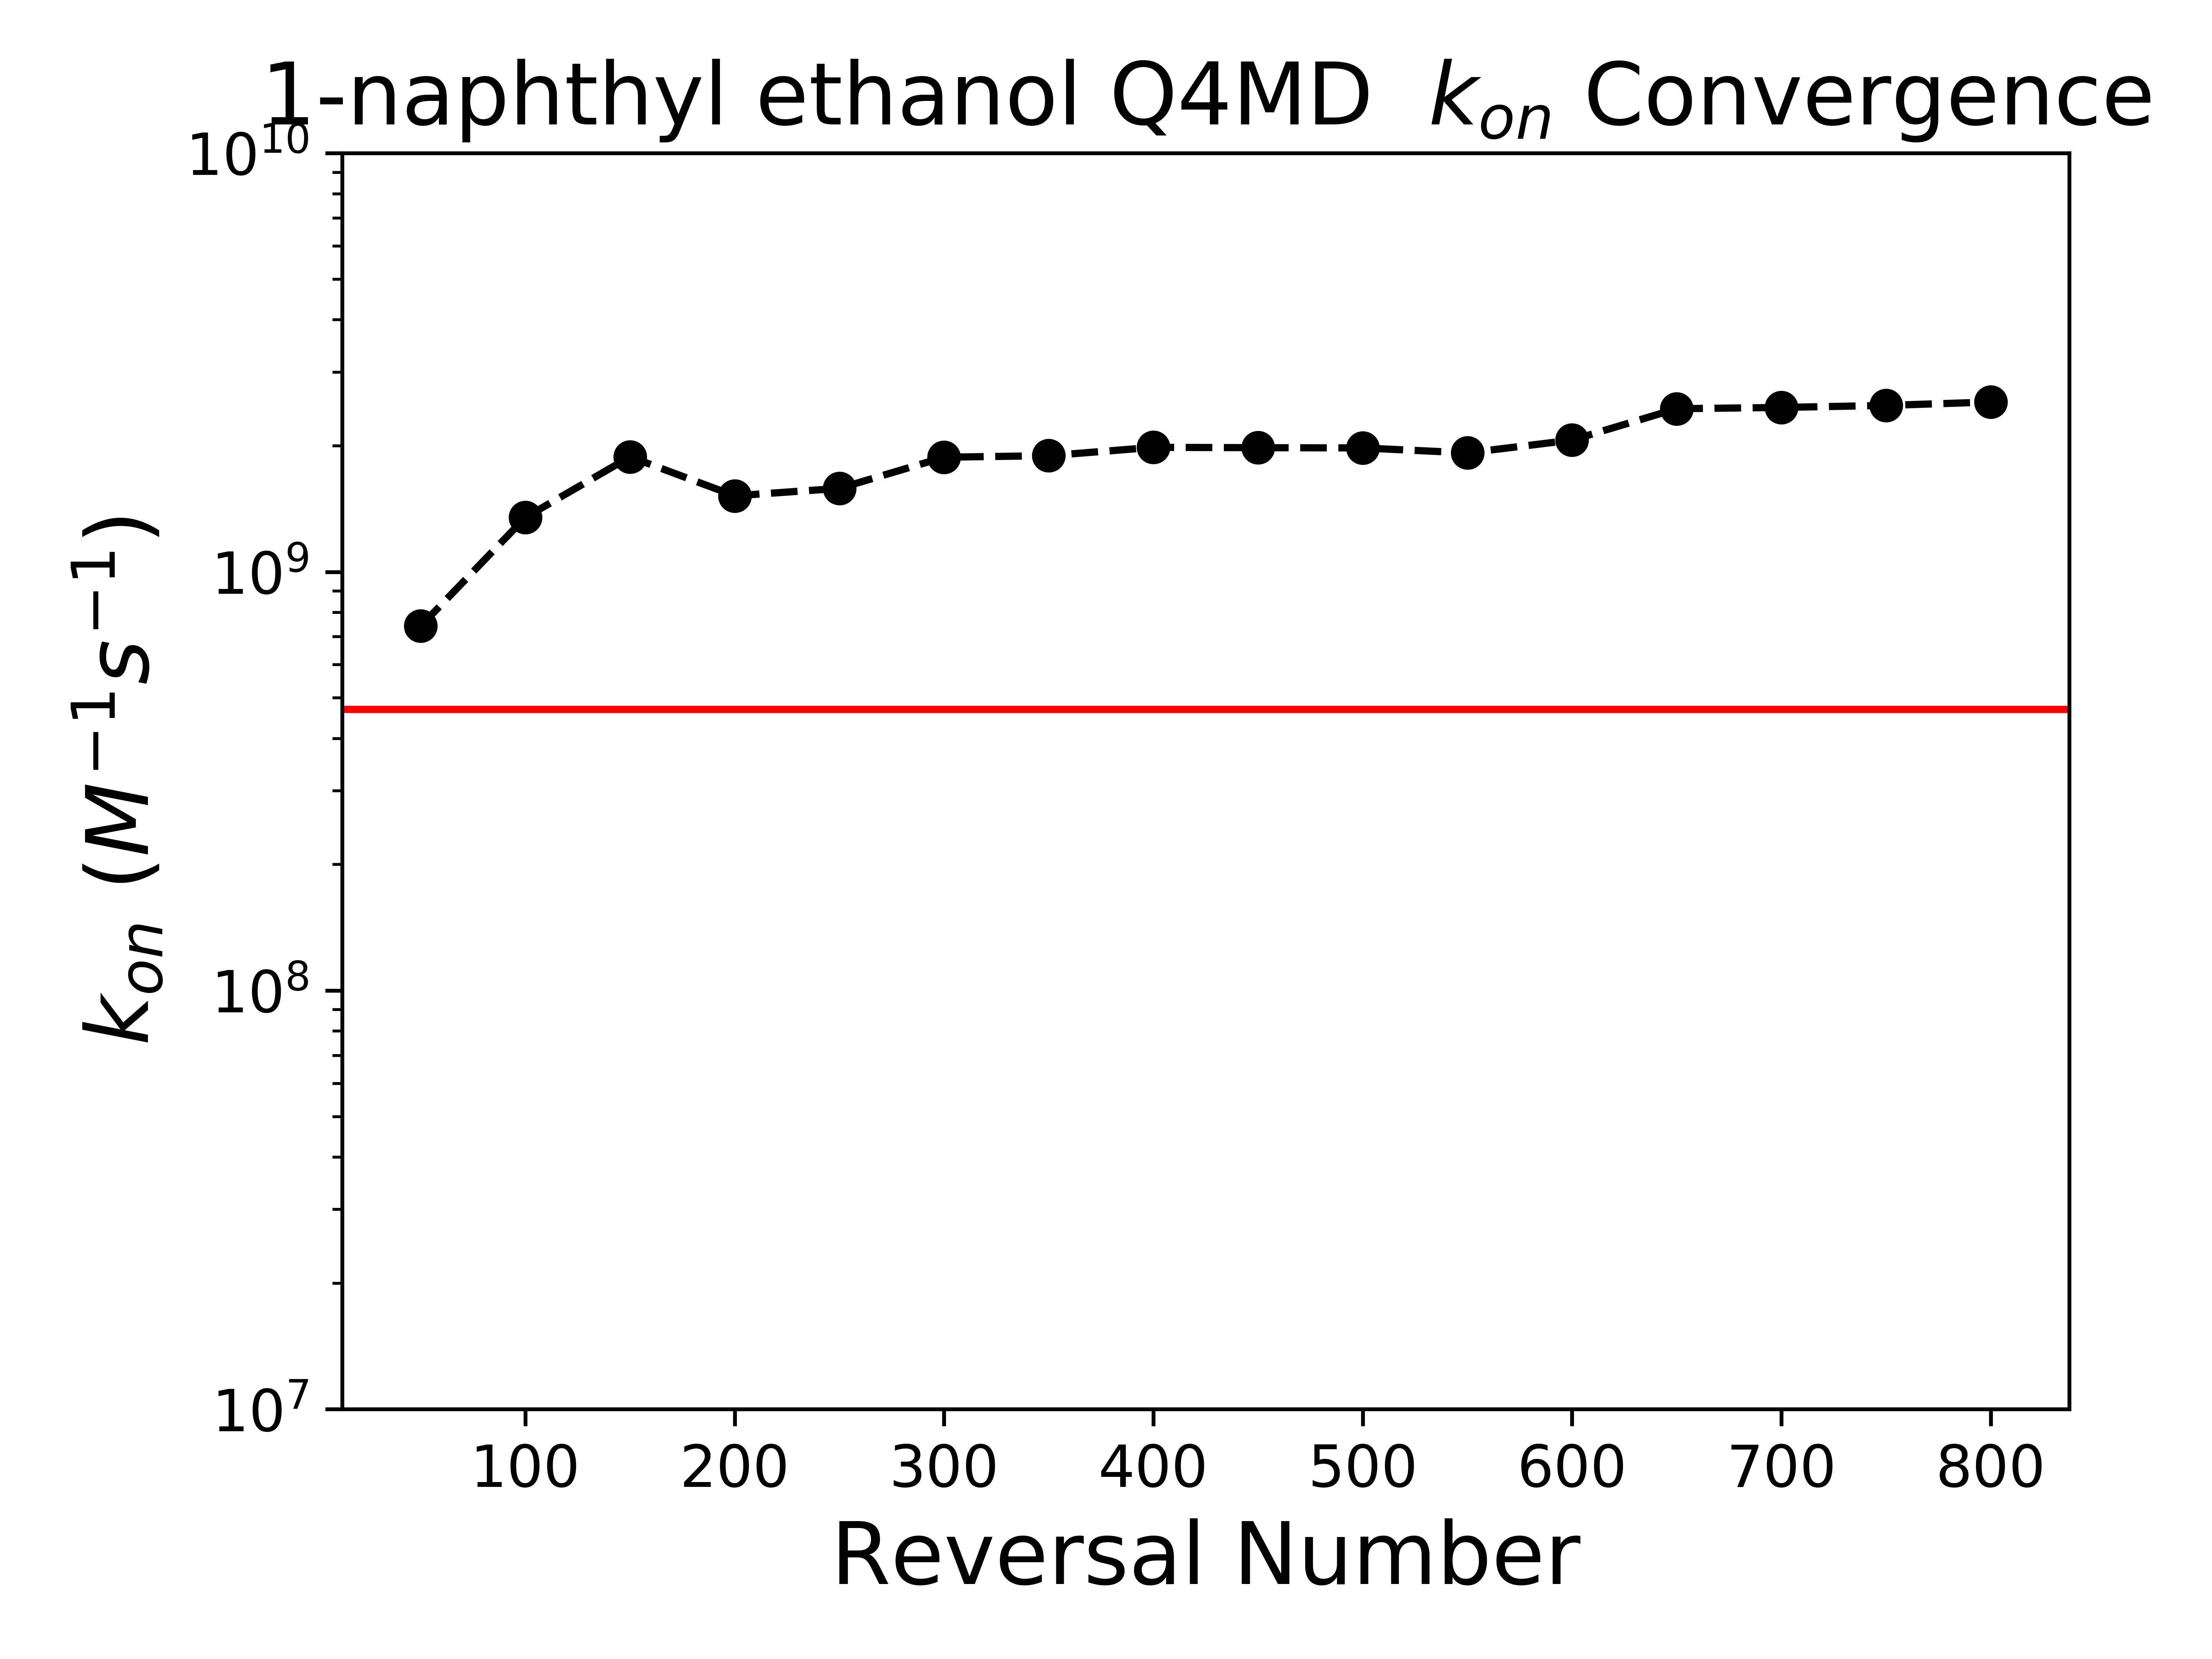
\includegraphics[width=\linewidth]{high_res_images/q4md_rate_conv_images/1-naphthylethanol_q4md_on_conv.png}
	\end{subfigure}
	\begin{subfigure}{0.3\linewidth}
		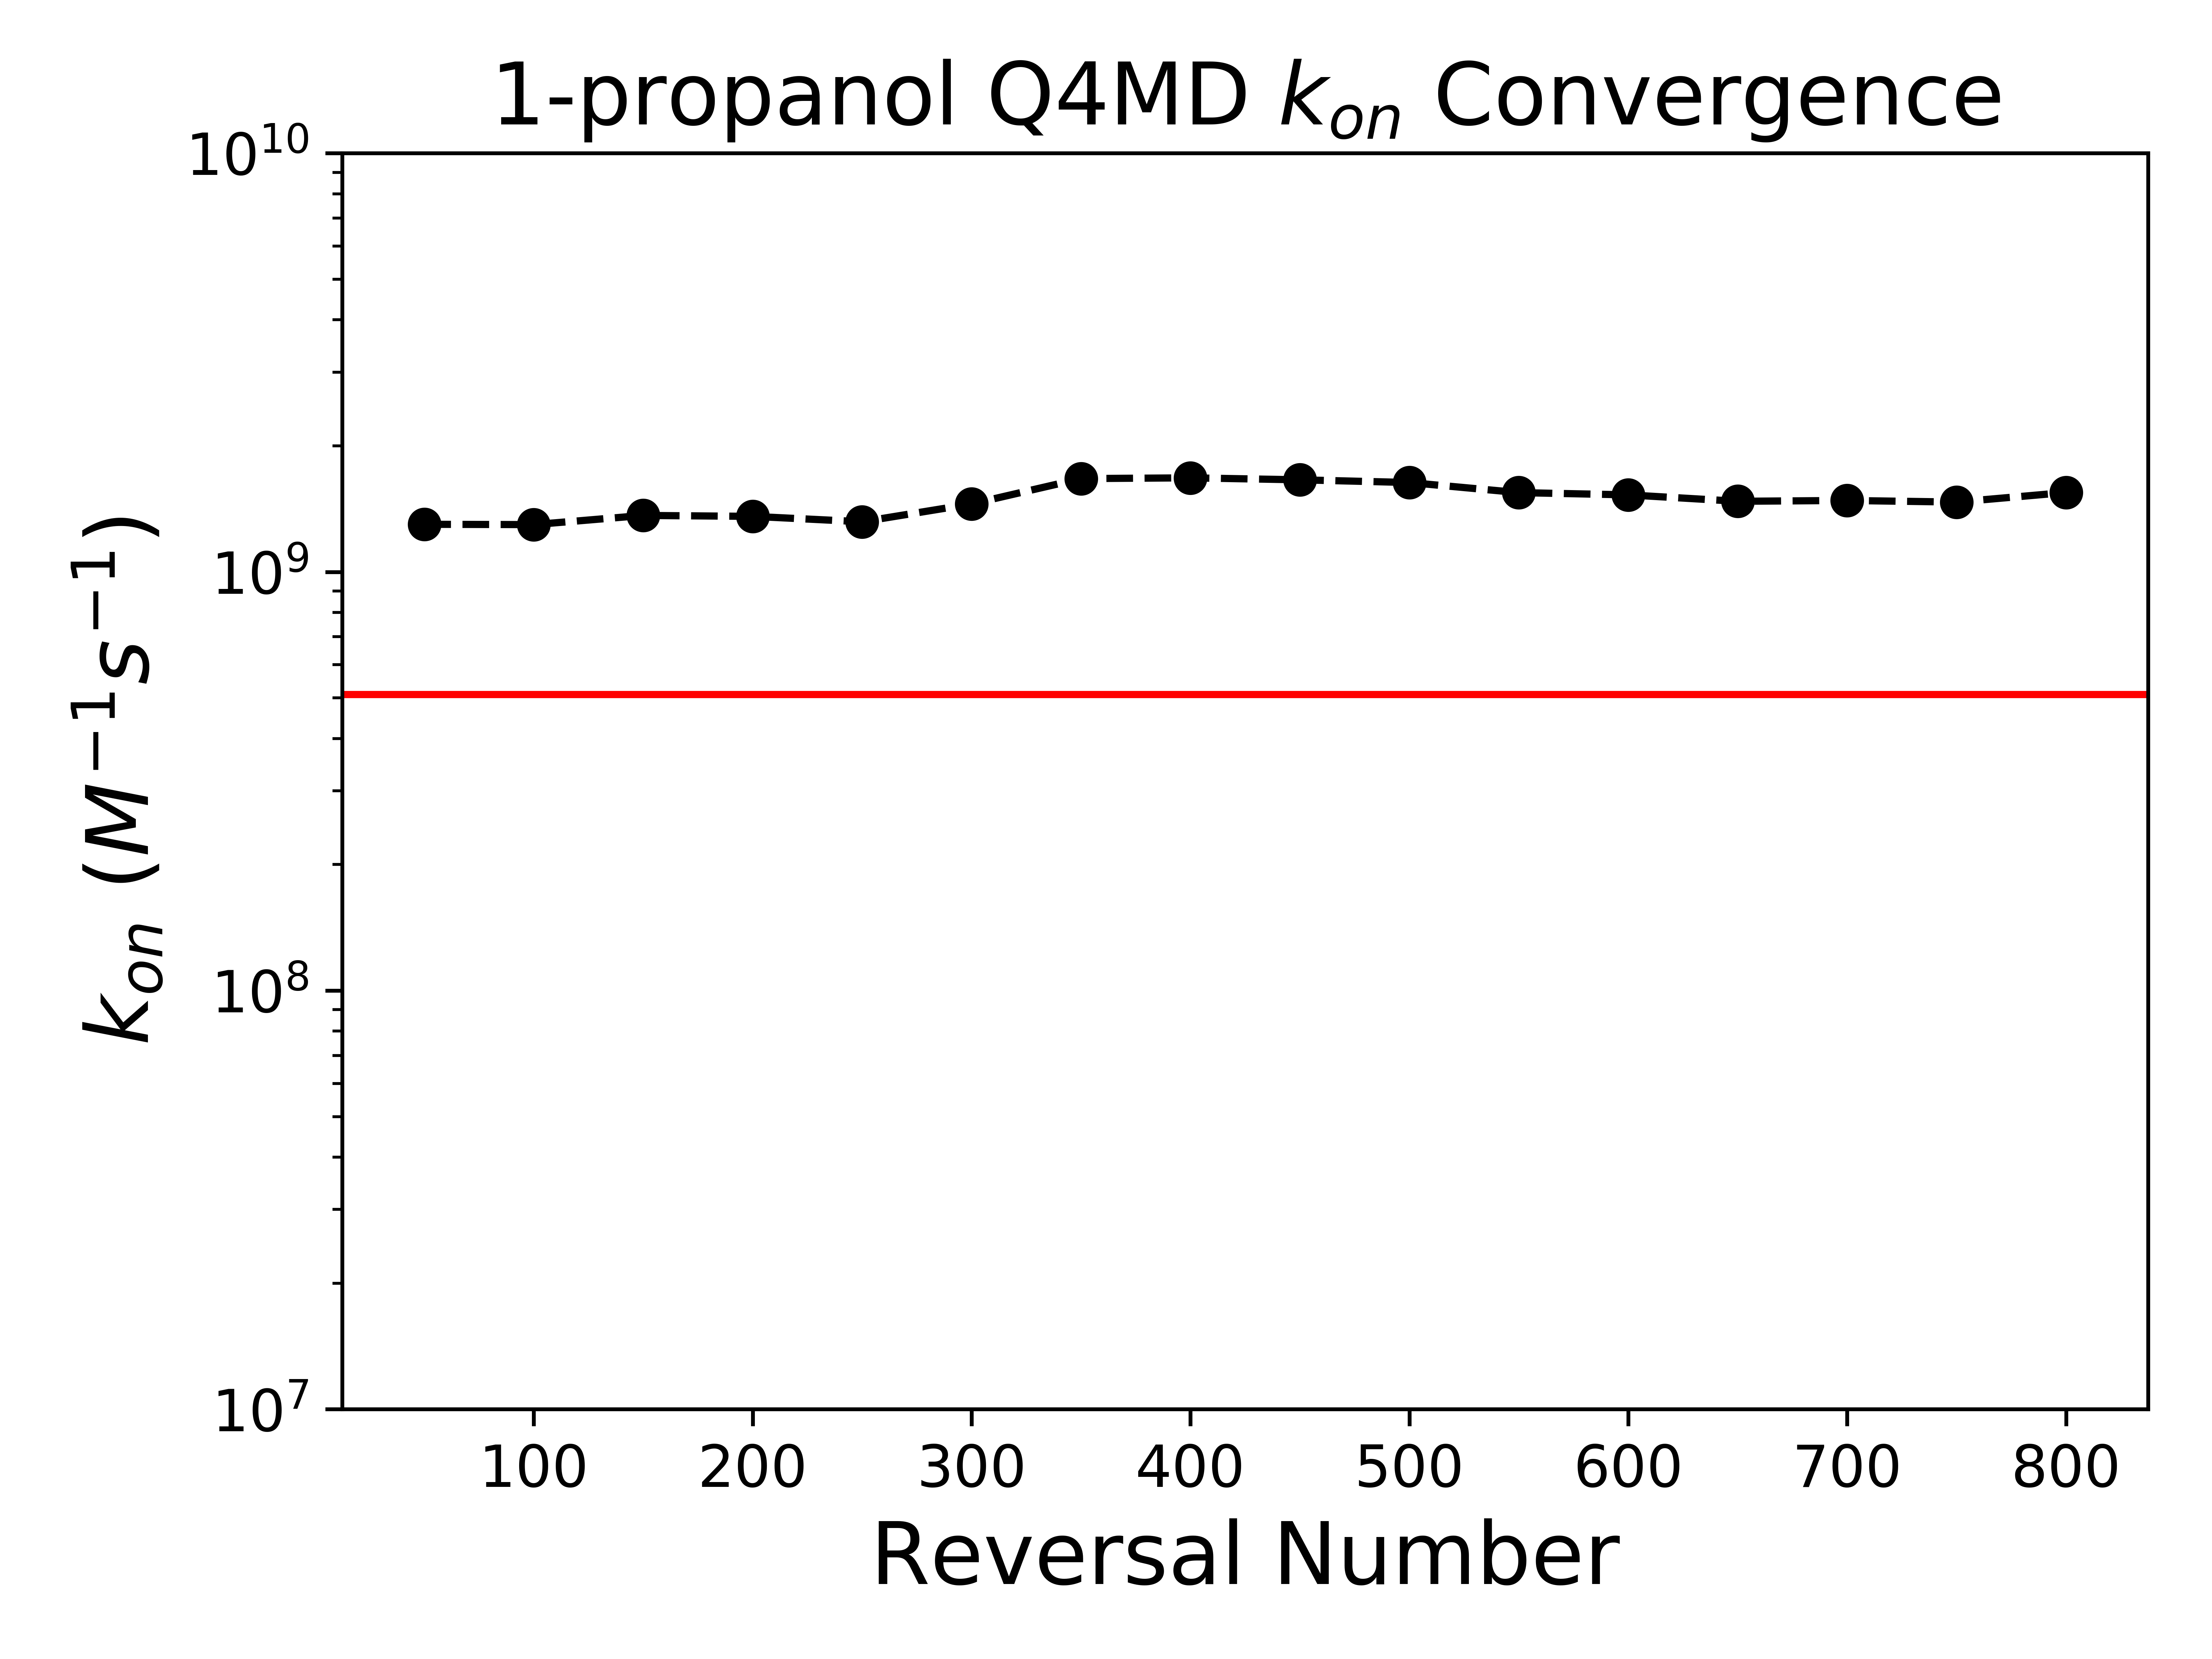
\includegraphics[width=\linewidth]{high_res_images/q4md_rate_conv_images/1-propanol_q4md_on_conv.png}
	\end{subfigure}
	\begin{subfigure}{0.3\linewidth}
		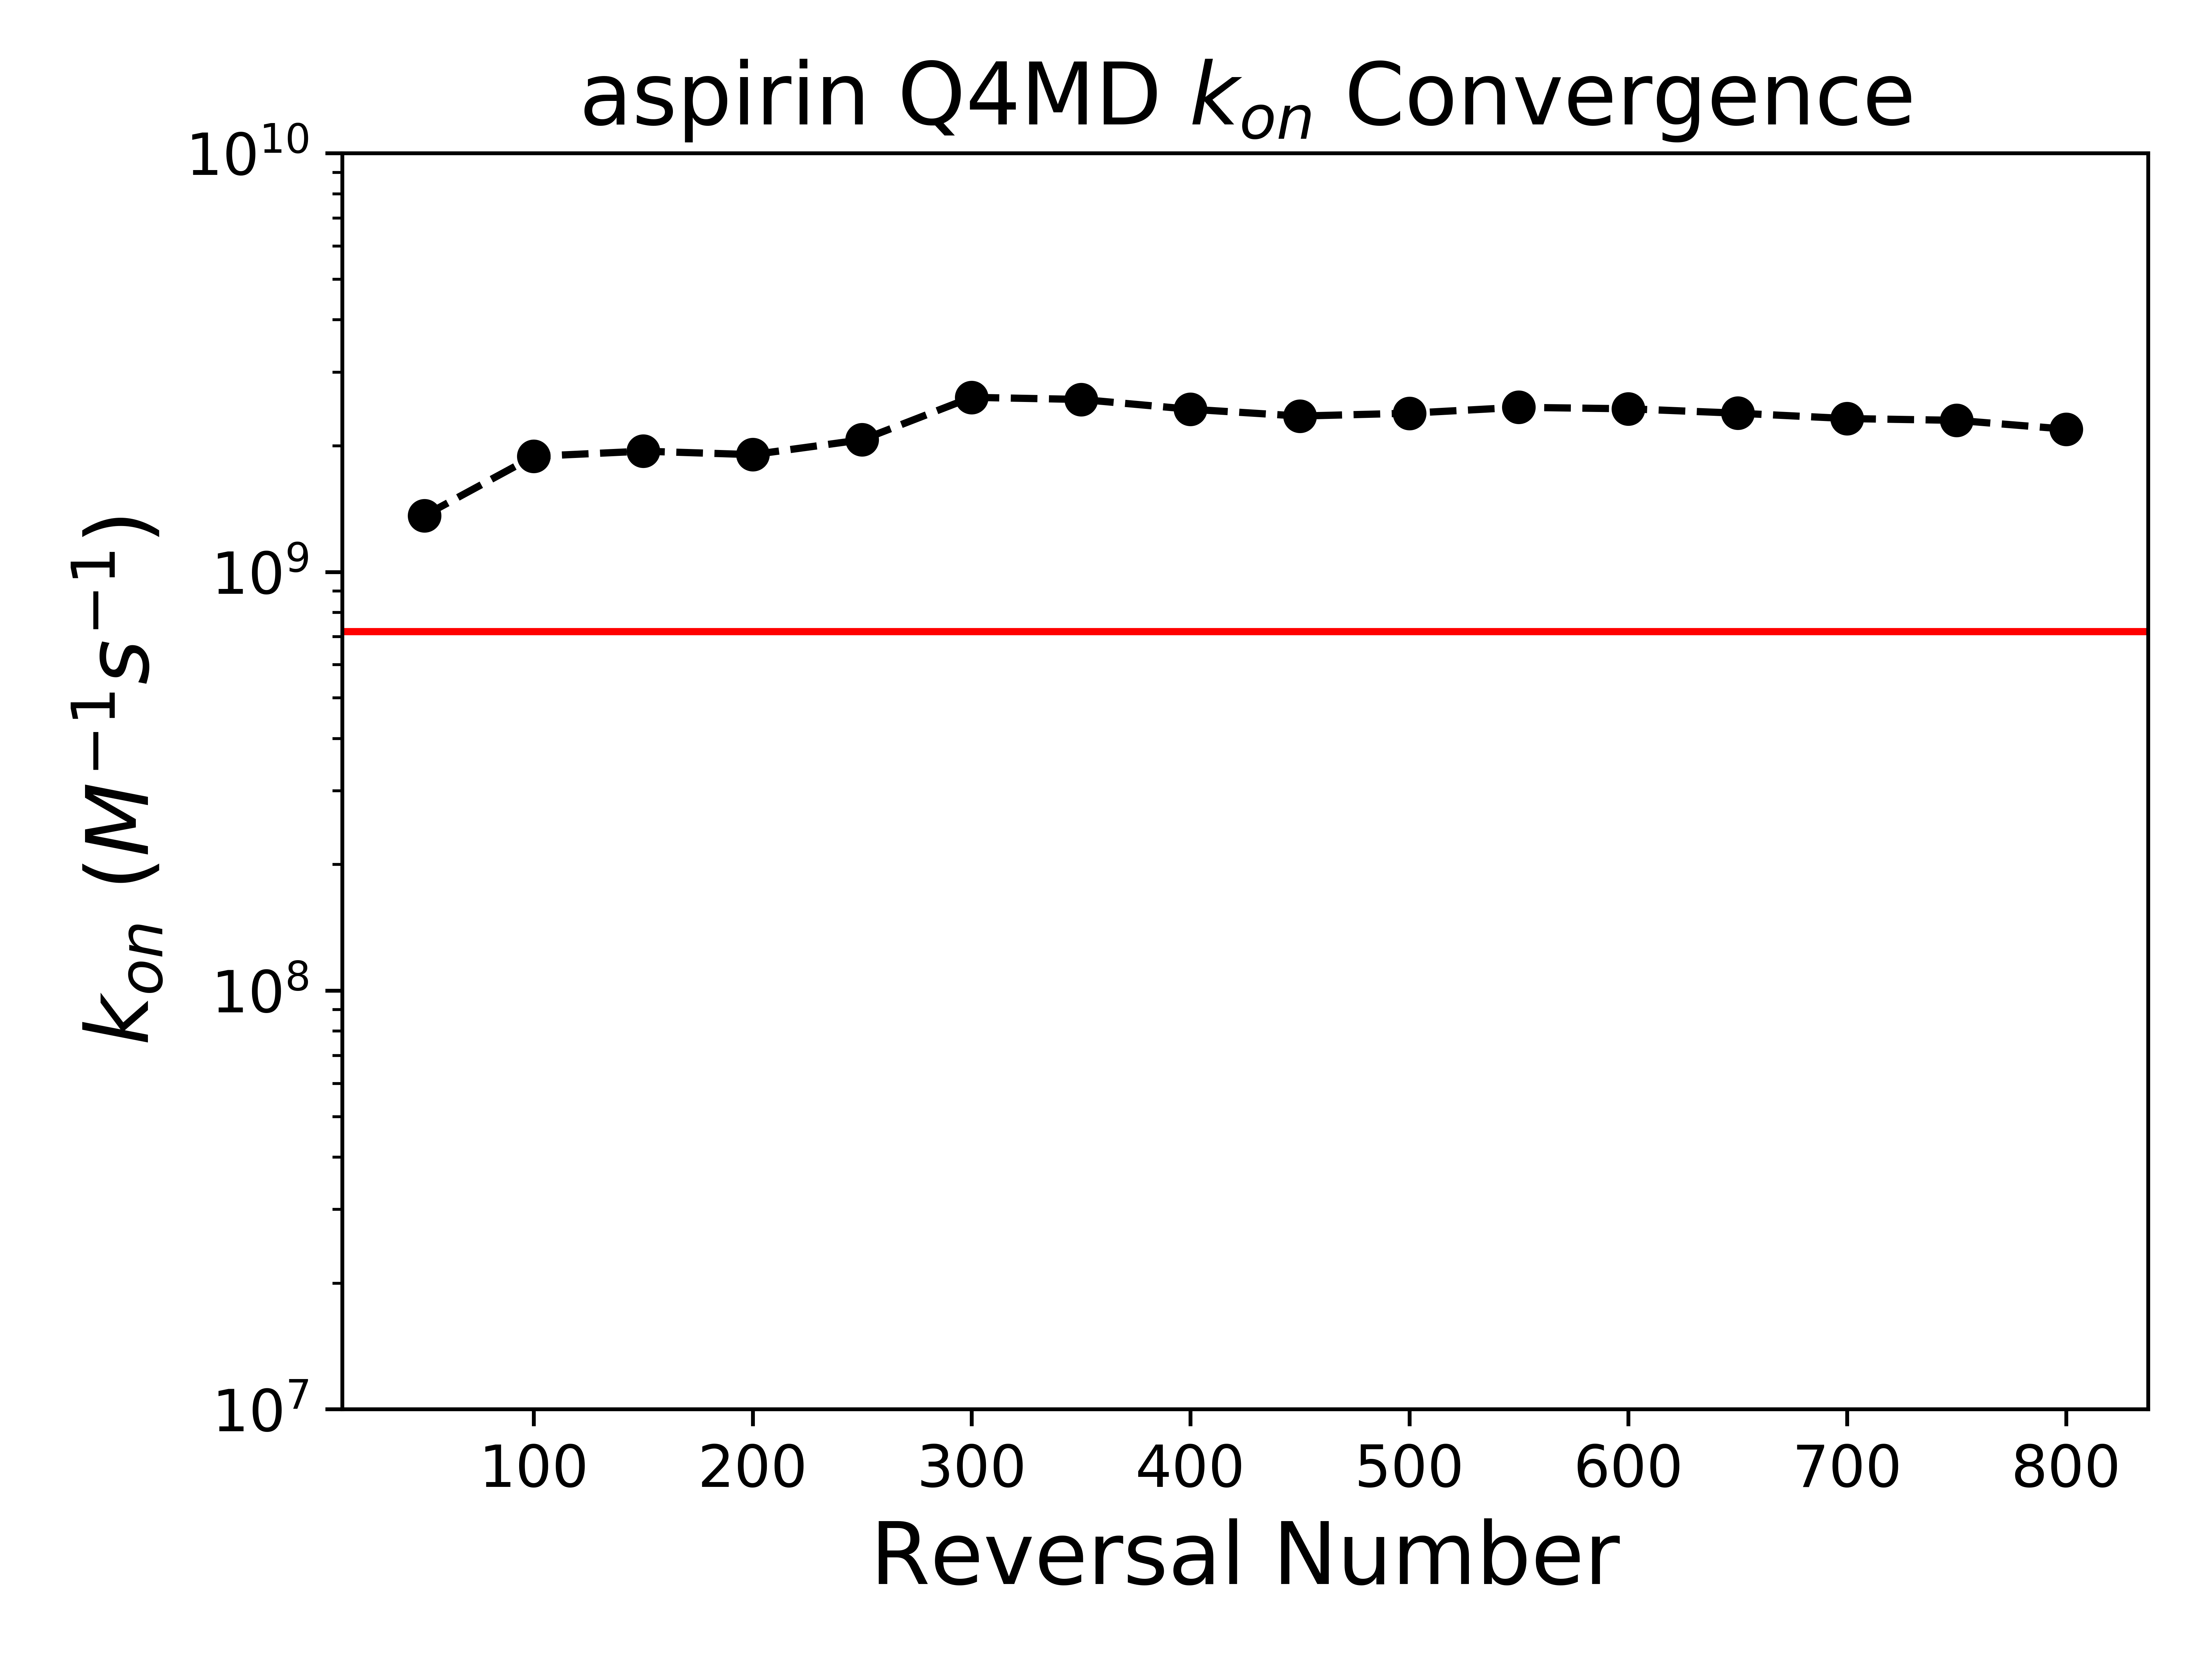
\includegraphics[width=\linewidth]{high_res_images/q4md_rate_conv_images/aspirin_q4md_on_conv.png}
	\end{subfigure}
	\caption{Convergence of on rates as a function of the number of reversals included using the Q4MD forcefield}
\end{figure}
%\begin{figure}
\begin{subfigure}{0.3\linewidth}
	\centering
	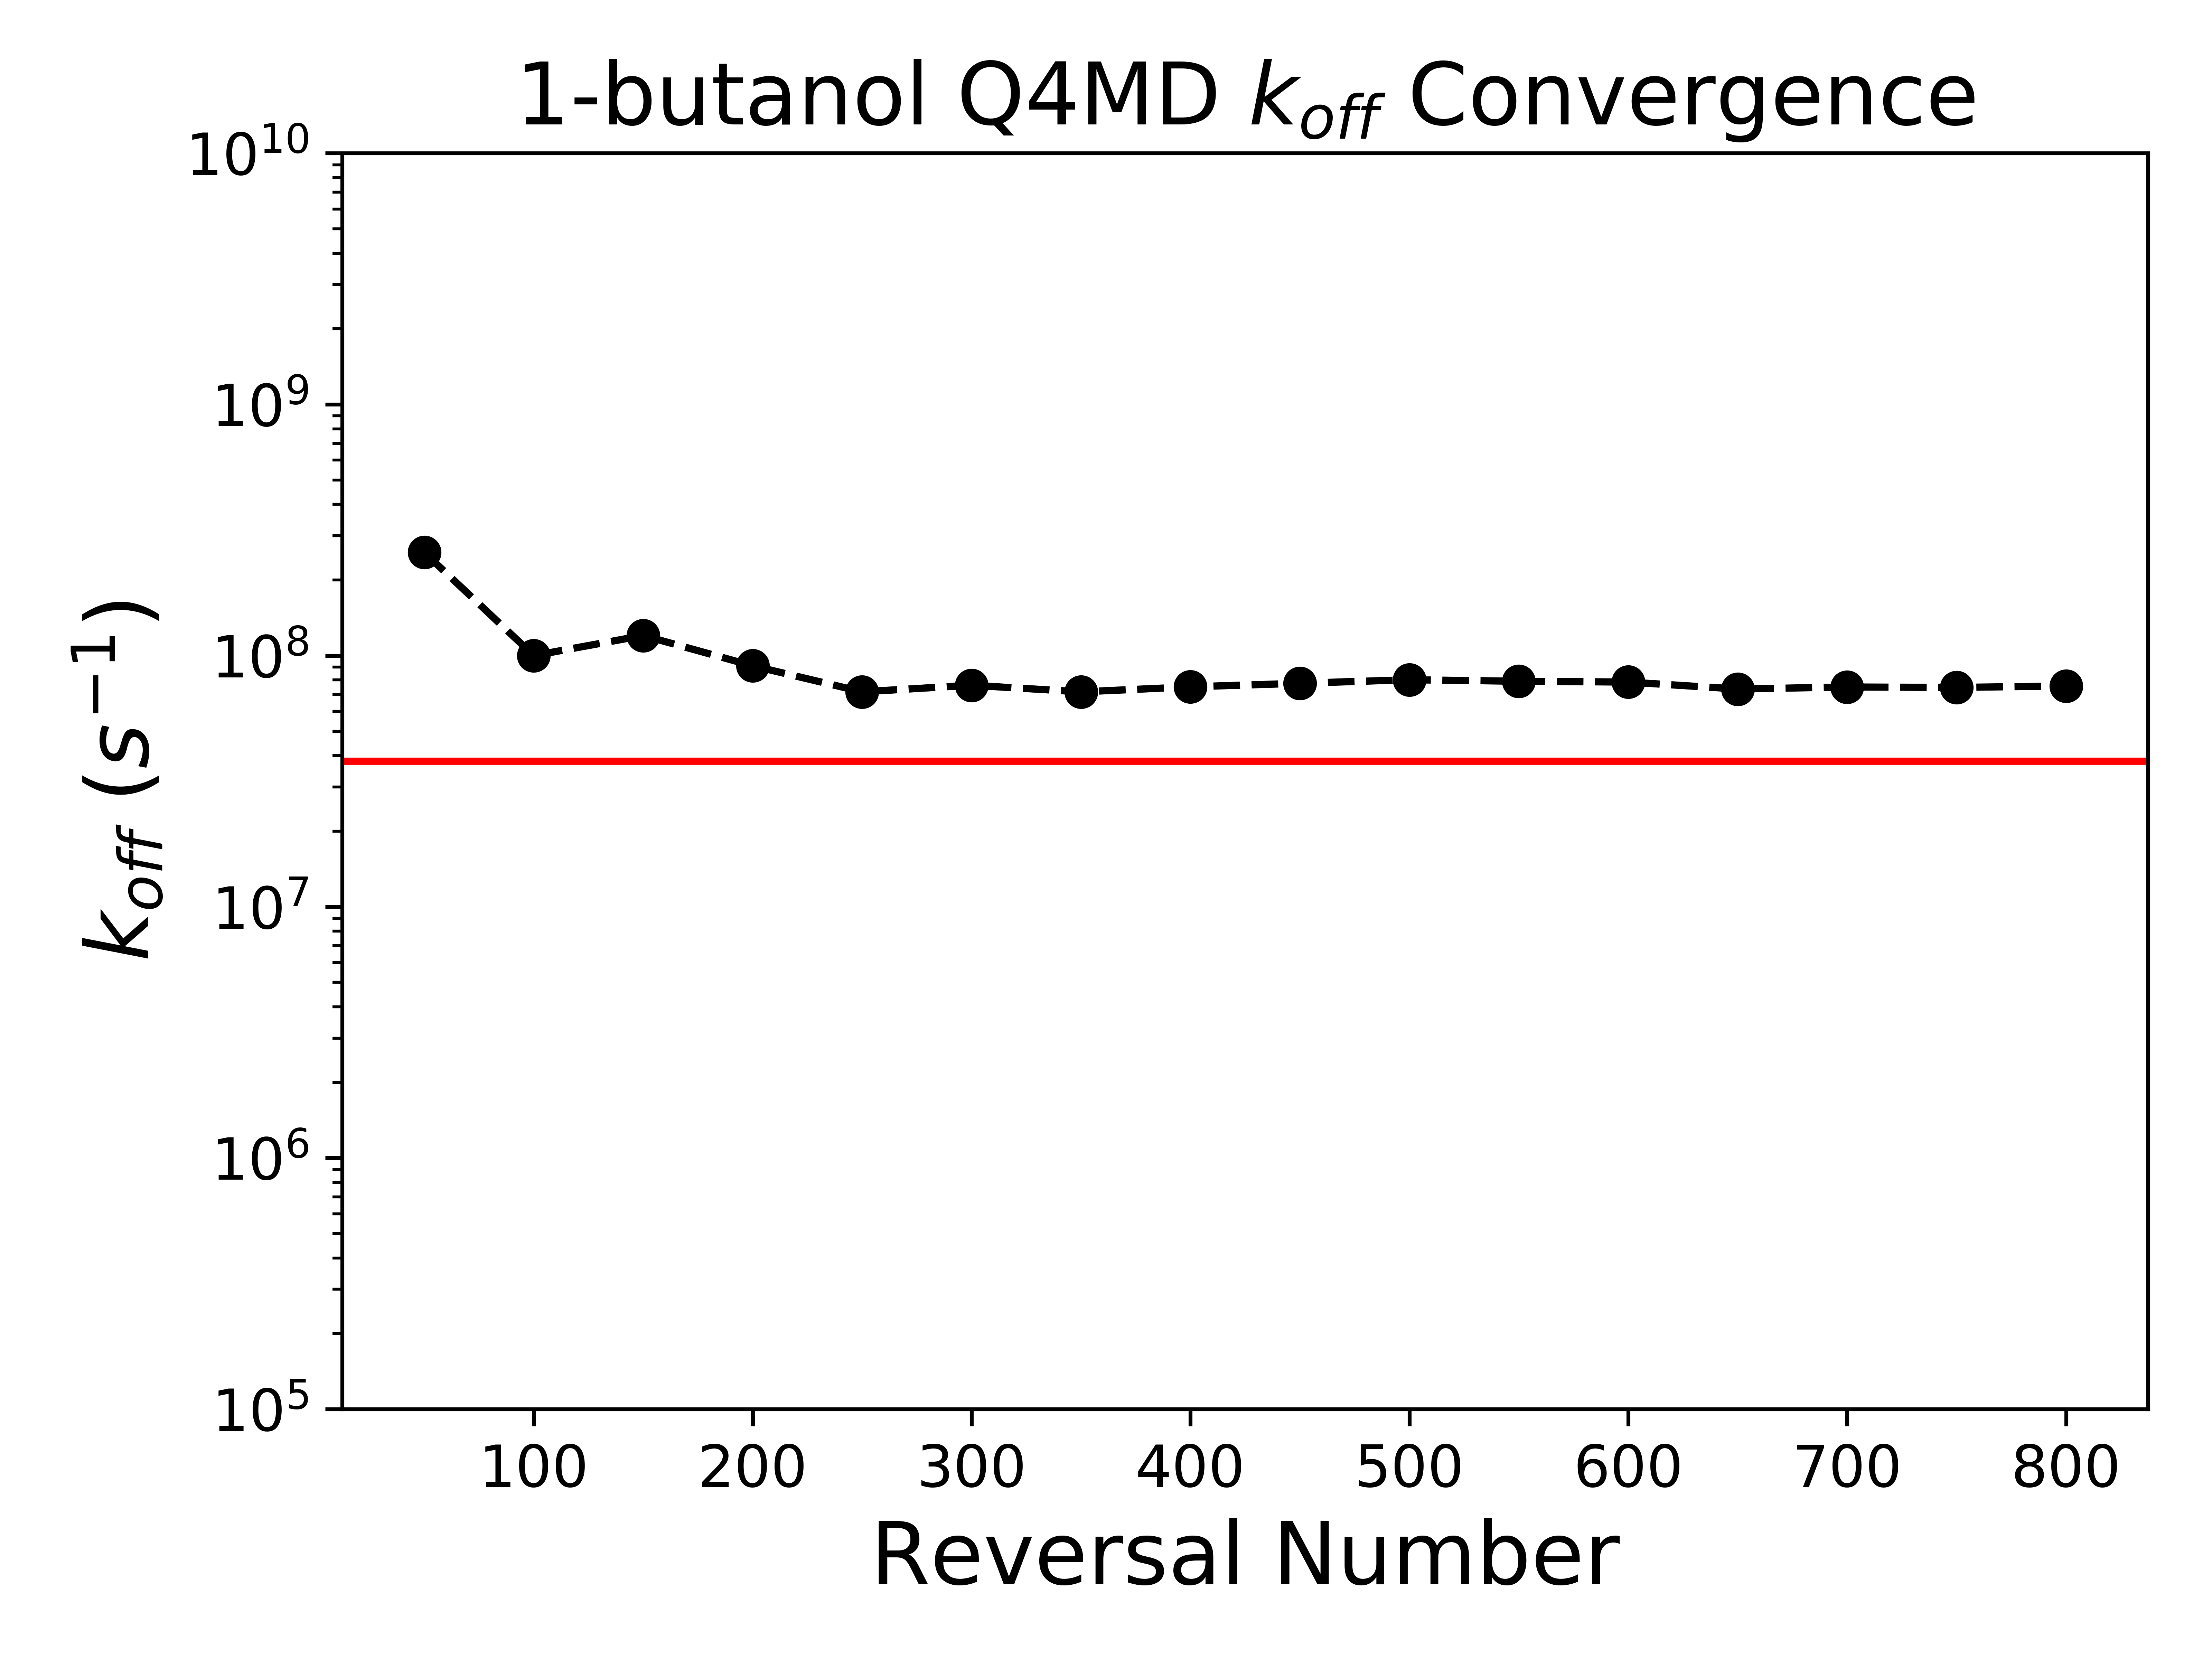
\includegraphics[width=\linewidth]{high_res_images/q4md_rate_conv_images/1-butanol_q4md_off_conv.png}
	\end{subfigure}%
\begin{subfigure}{0.3\linewidth}
		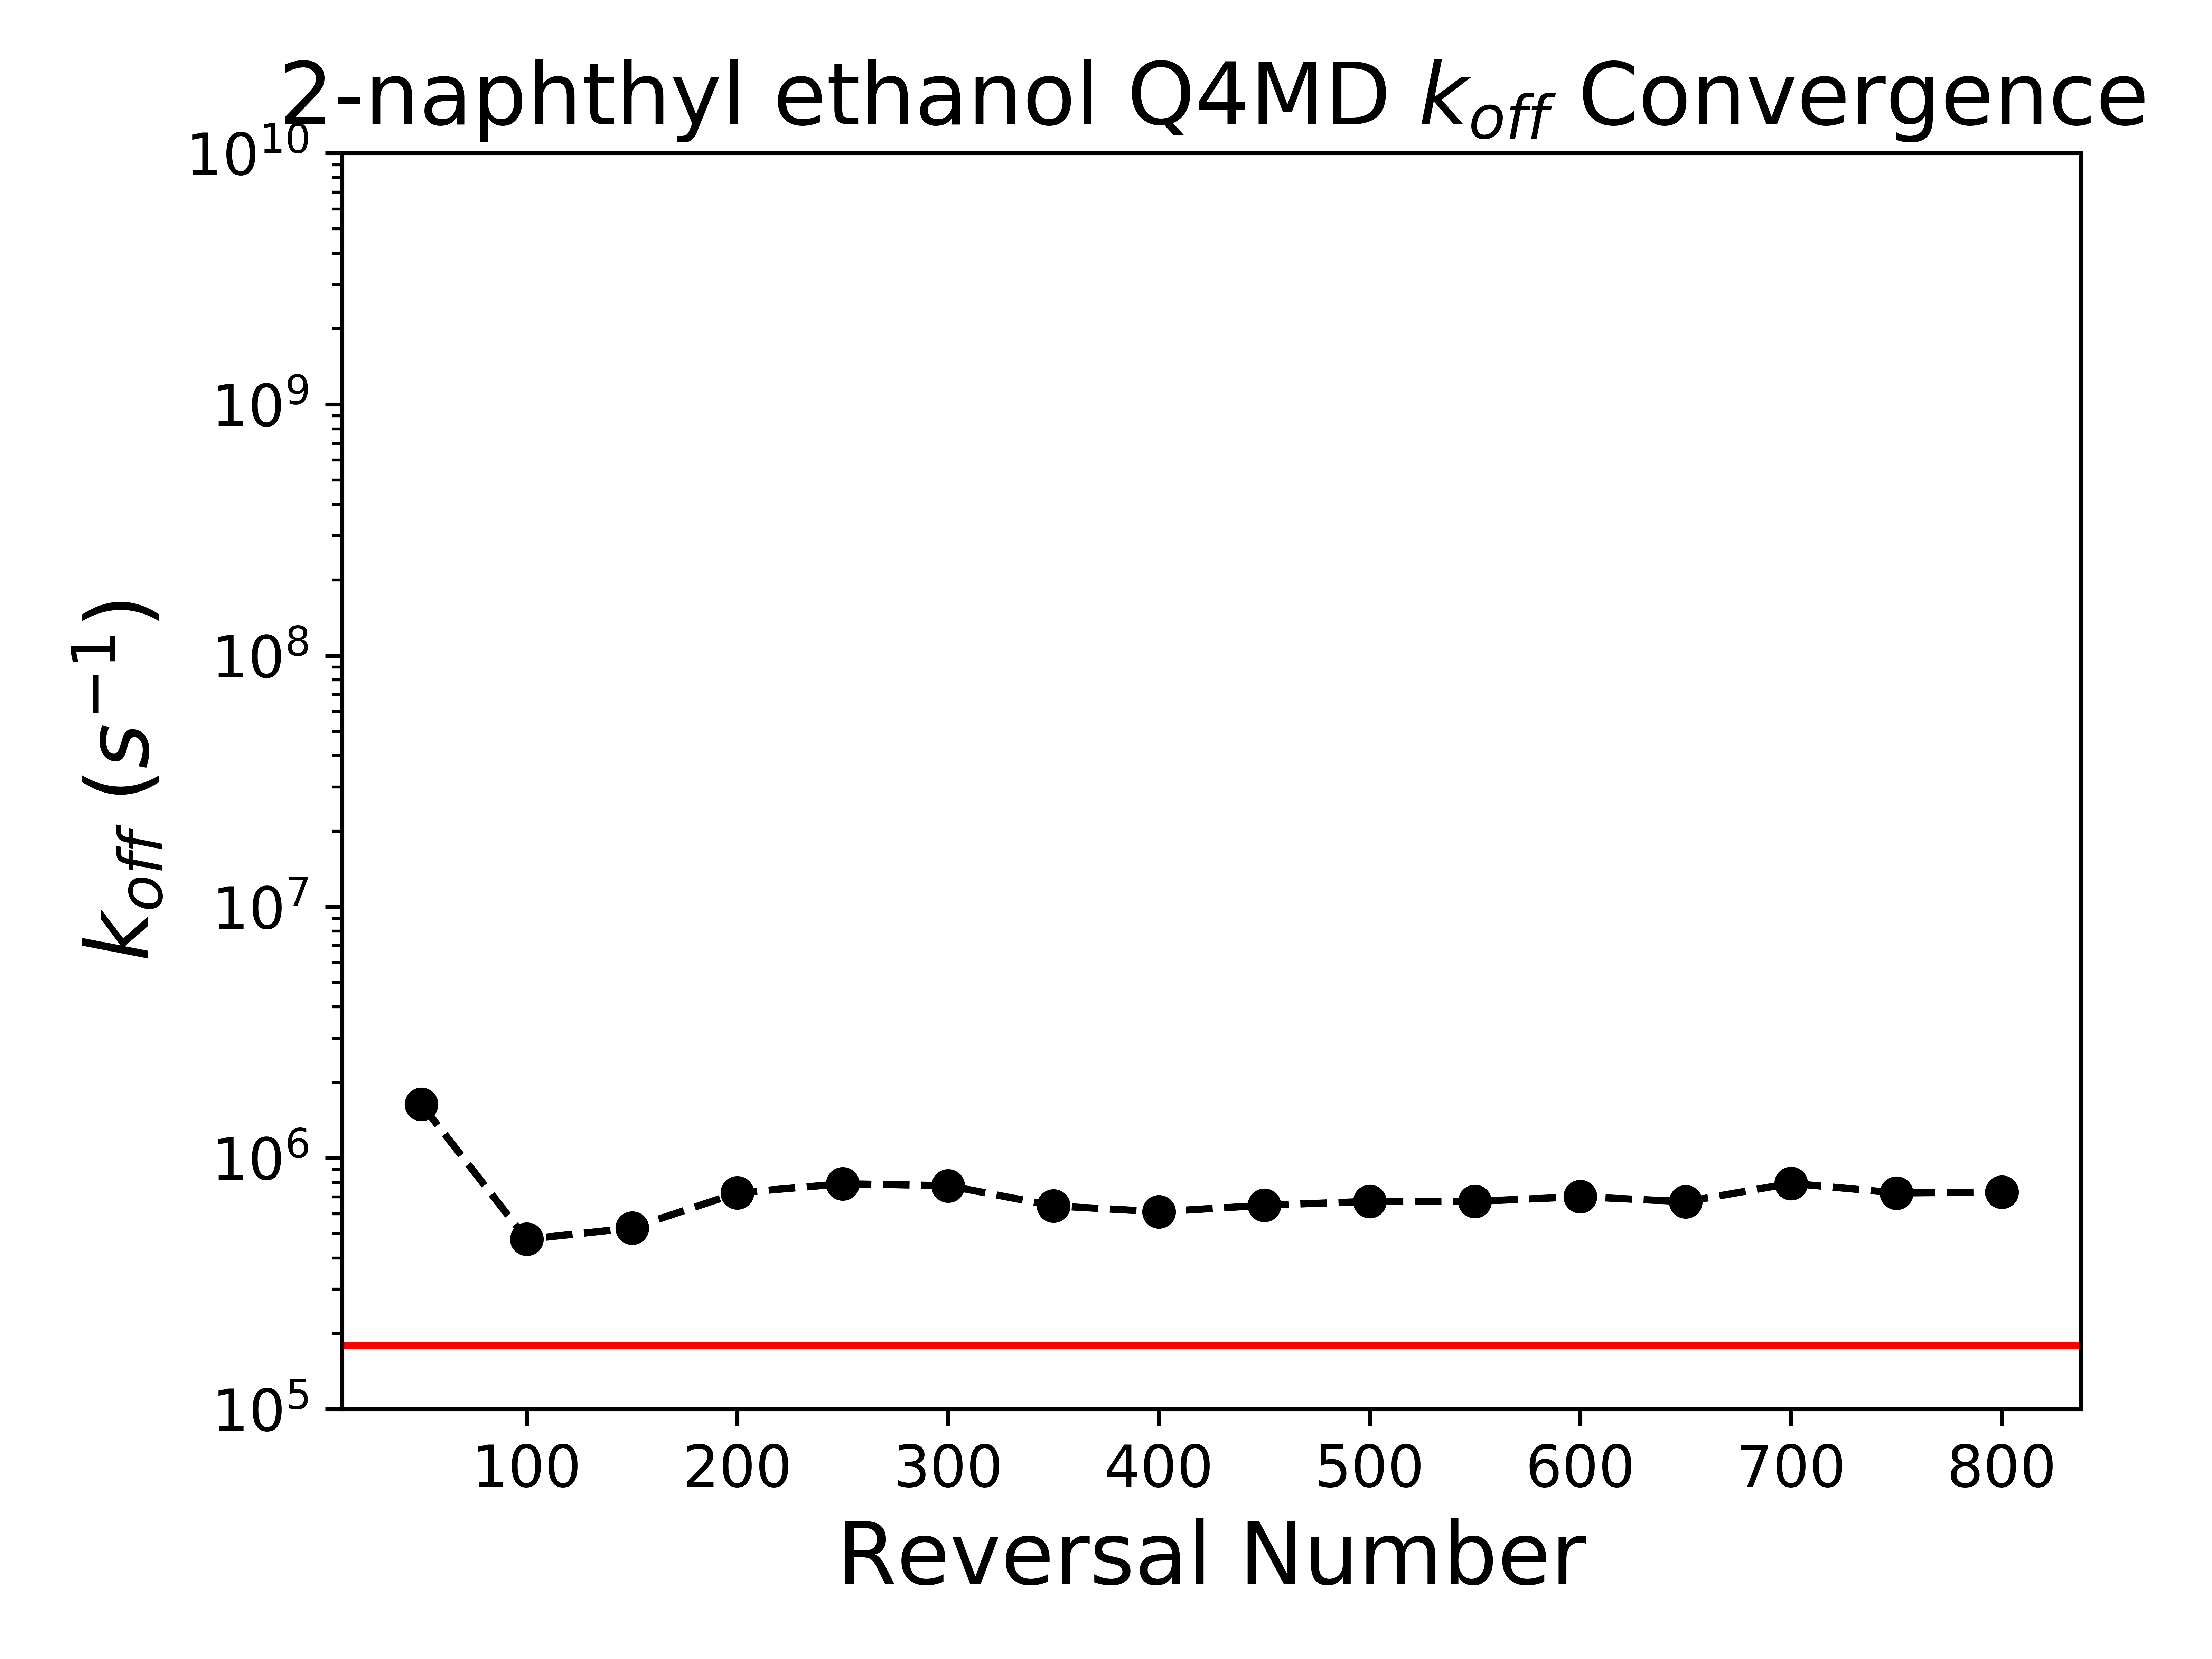
\includegraphics[width=\linewidth]{high_res_images/q4md_rate_conv_images/2-naphthylethanol_q4md_off_conv.png}
\end{subfigure}%
	\begin{subfigure}{0.3\linewidth}
		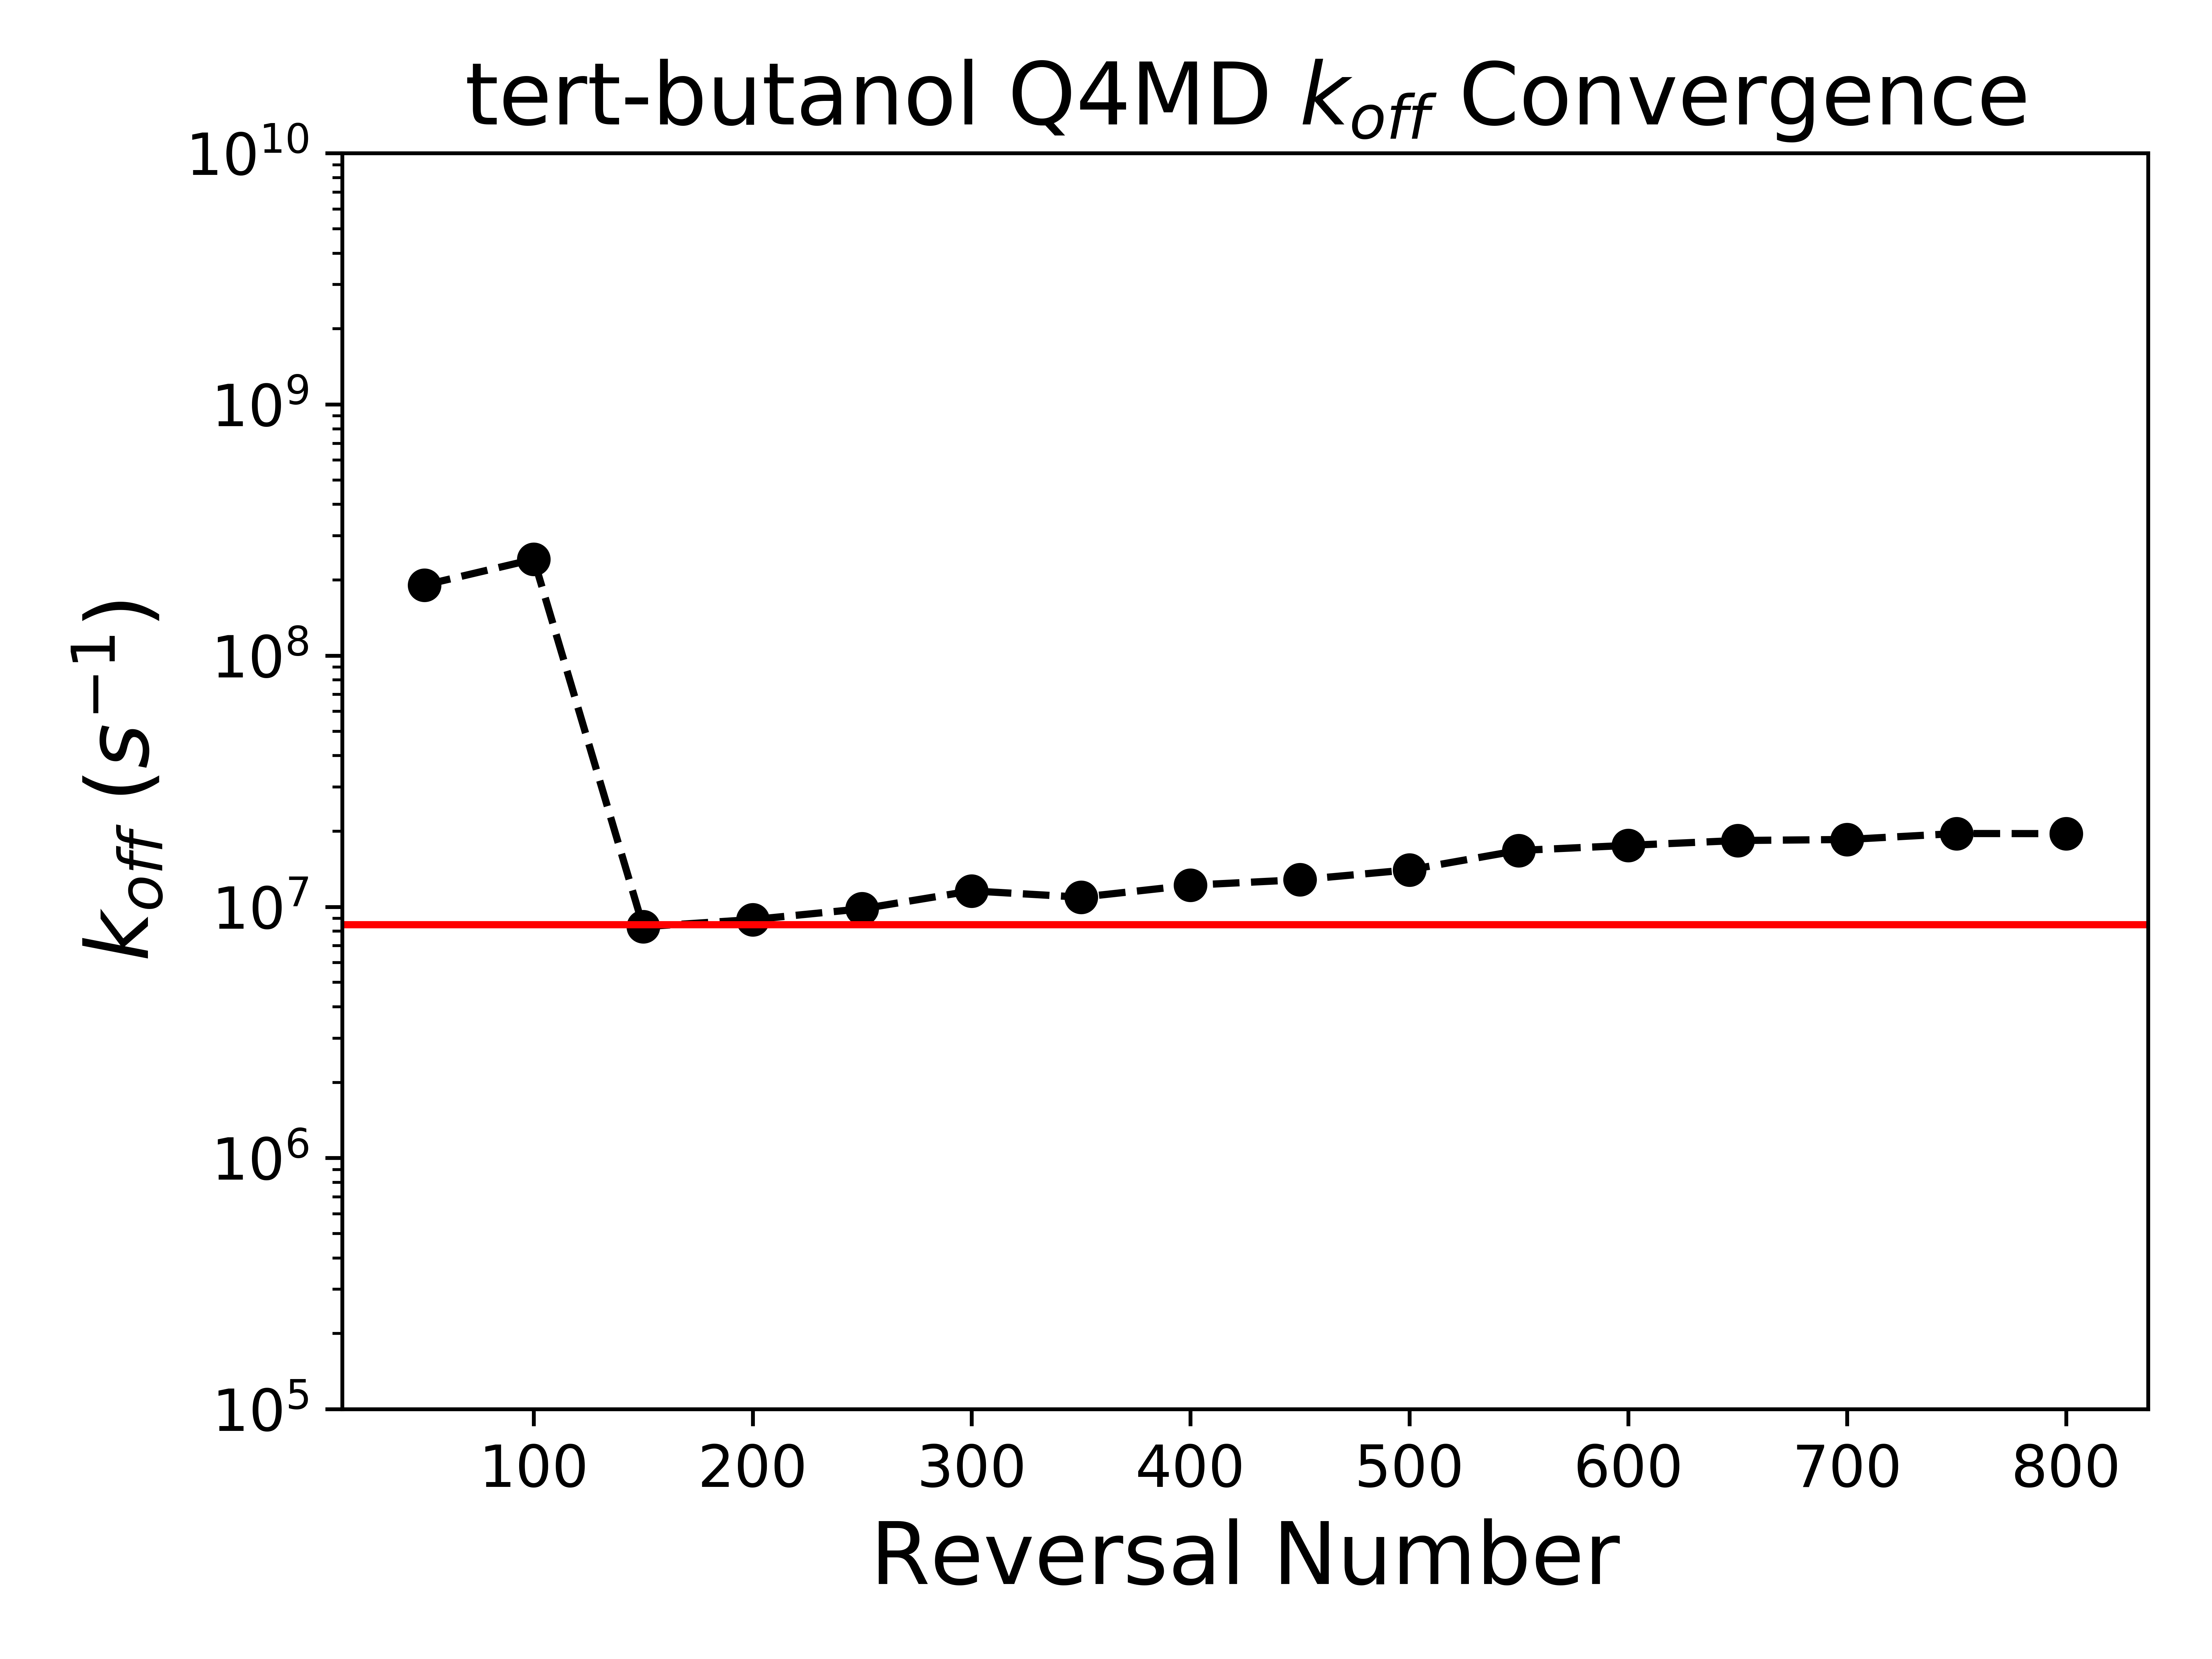
\includegraphics[width=\linewidth]{high_res_images/q4md_rate_conv_images/tert-butanol_q4md_off_conv.png}
	\end{subfigure}
	\begin{subfigure}{0.3\linewidth}
		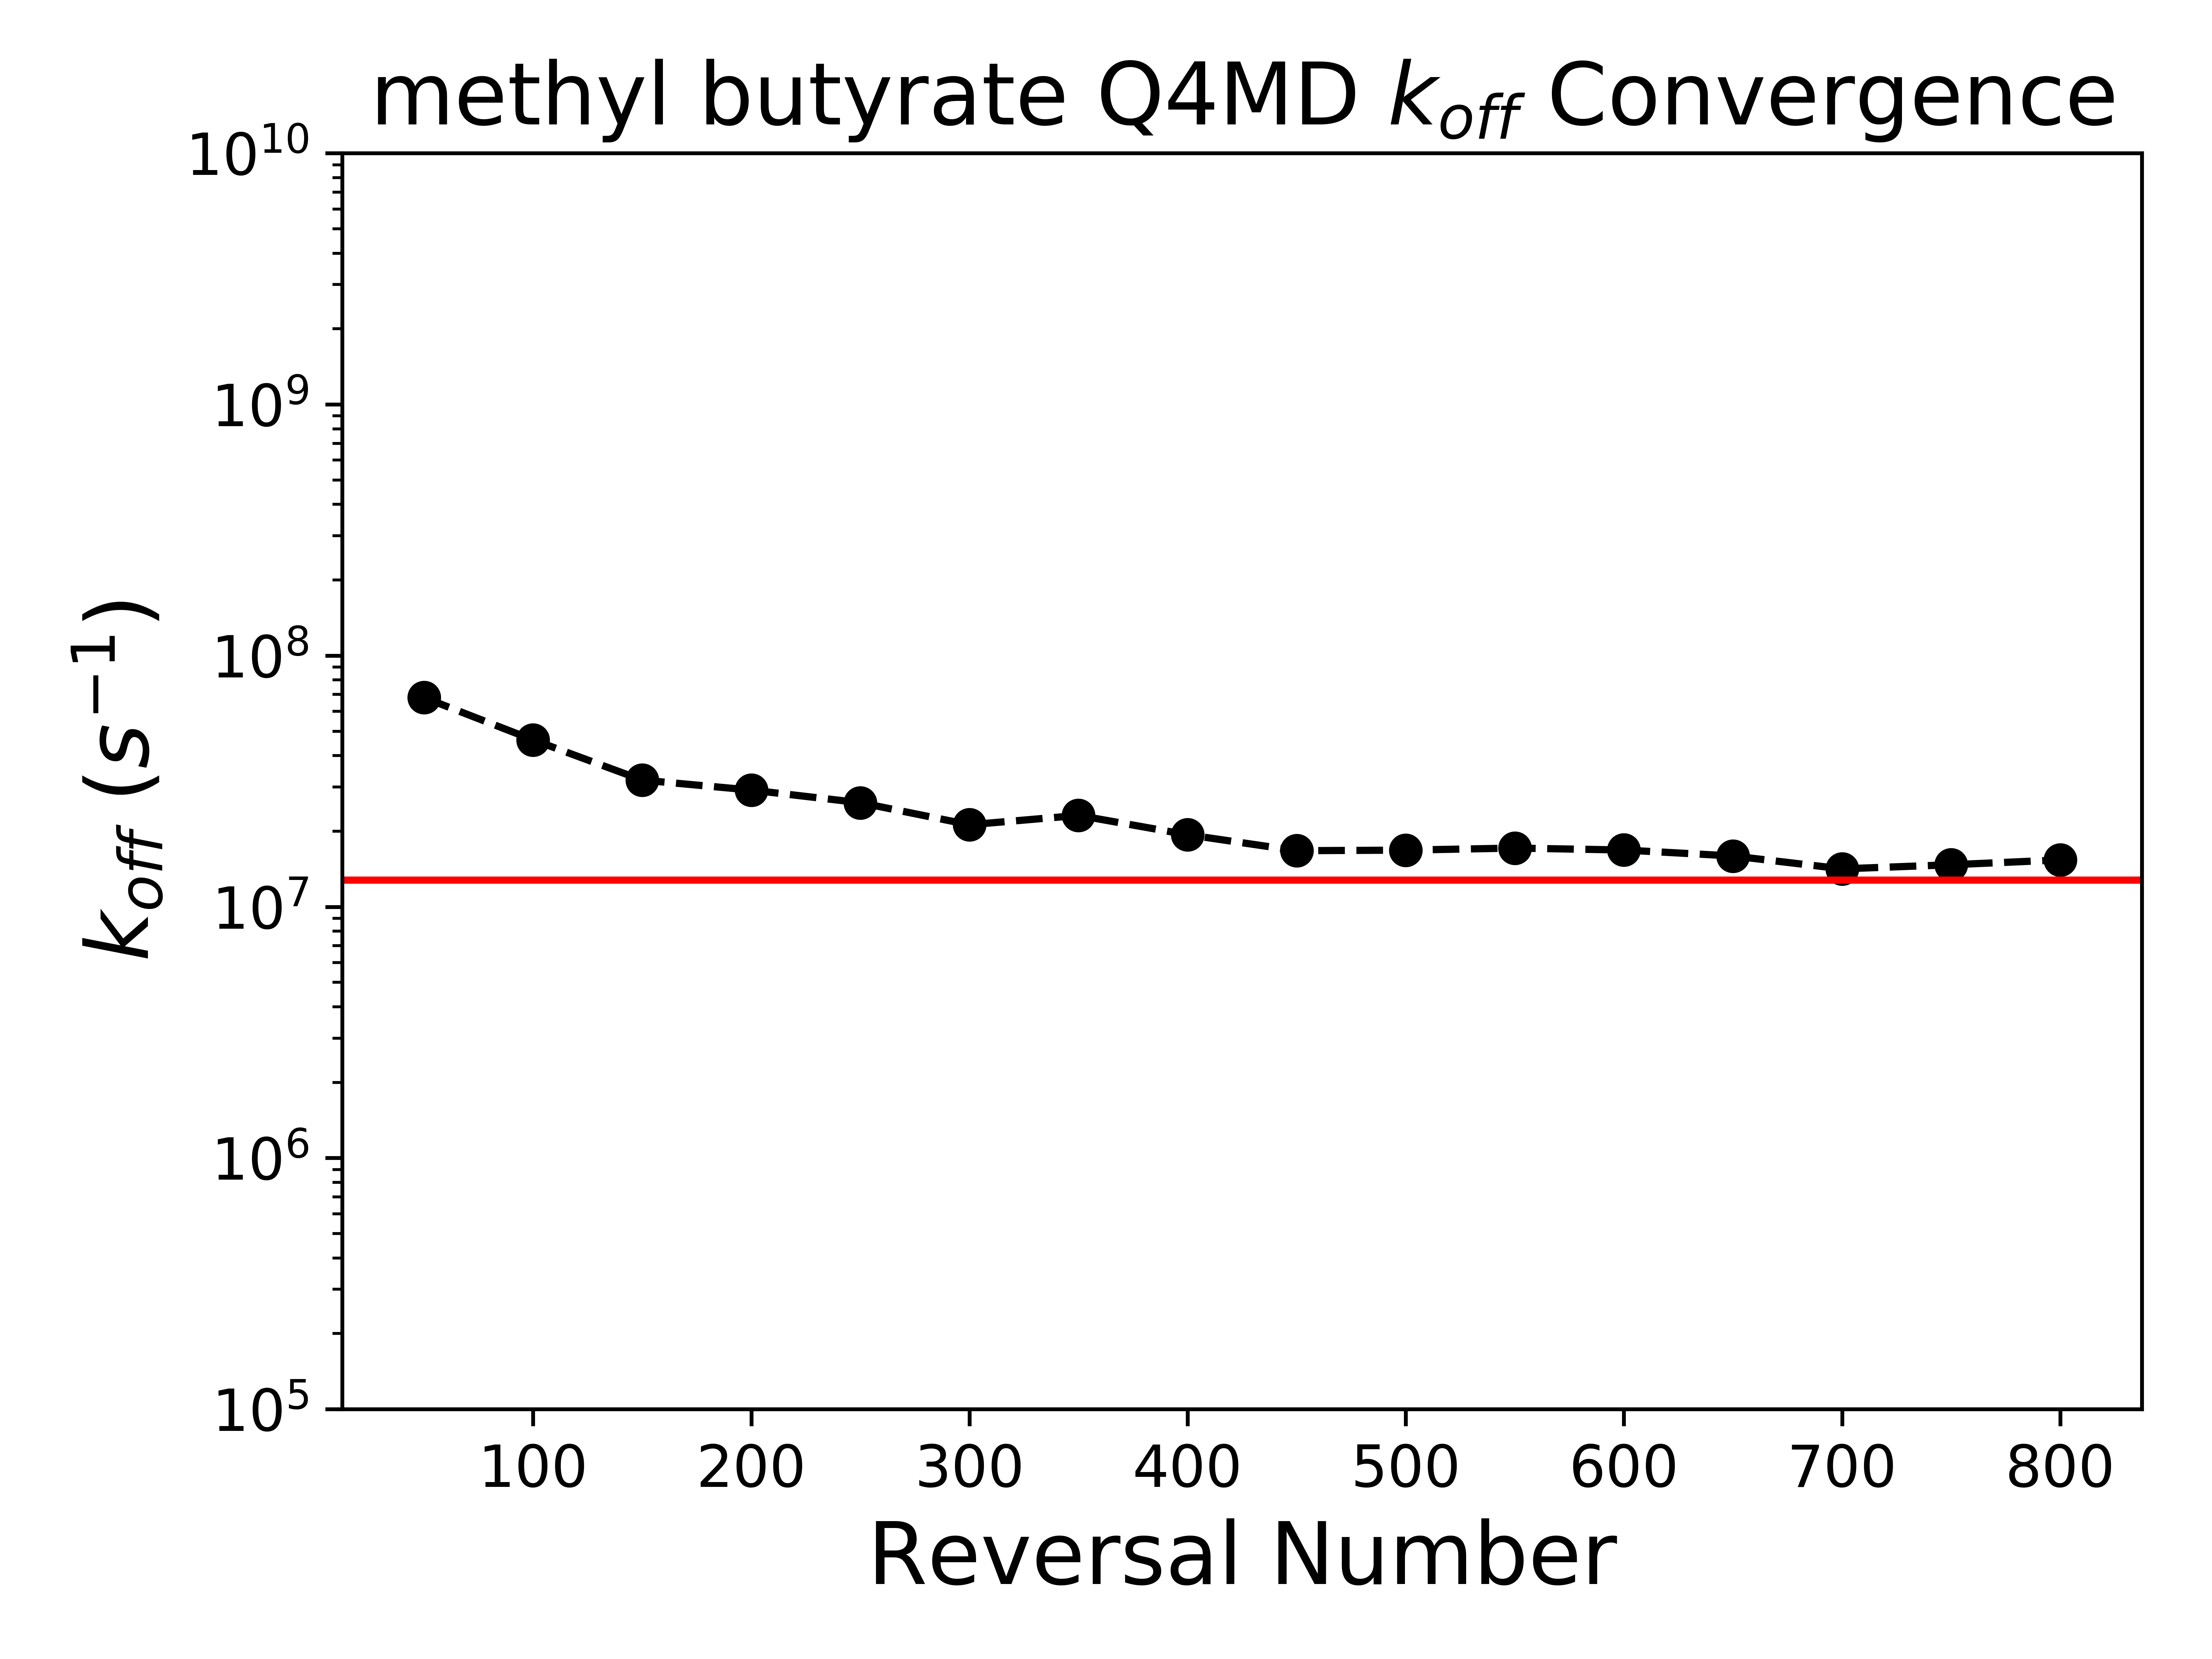
\includegraphics[width=\linewidth]{high_res_images/q4md_rate_conv_images/methylbutyrate_q4md_off_conv.png}
	\end{subfigure}
	\begin{subfigure}{0.3\linewidth}
		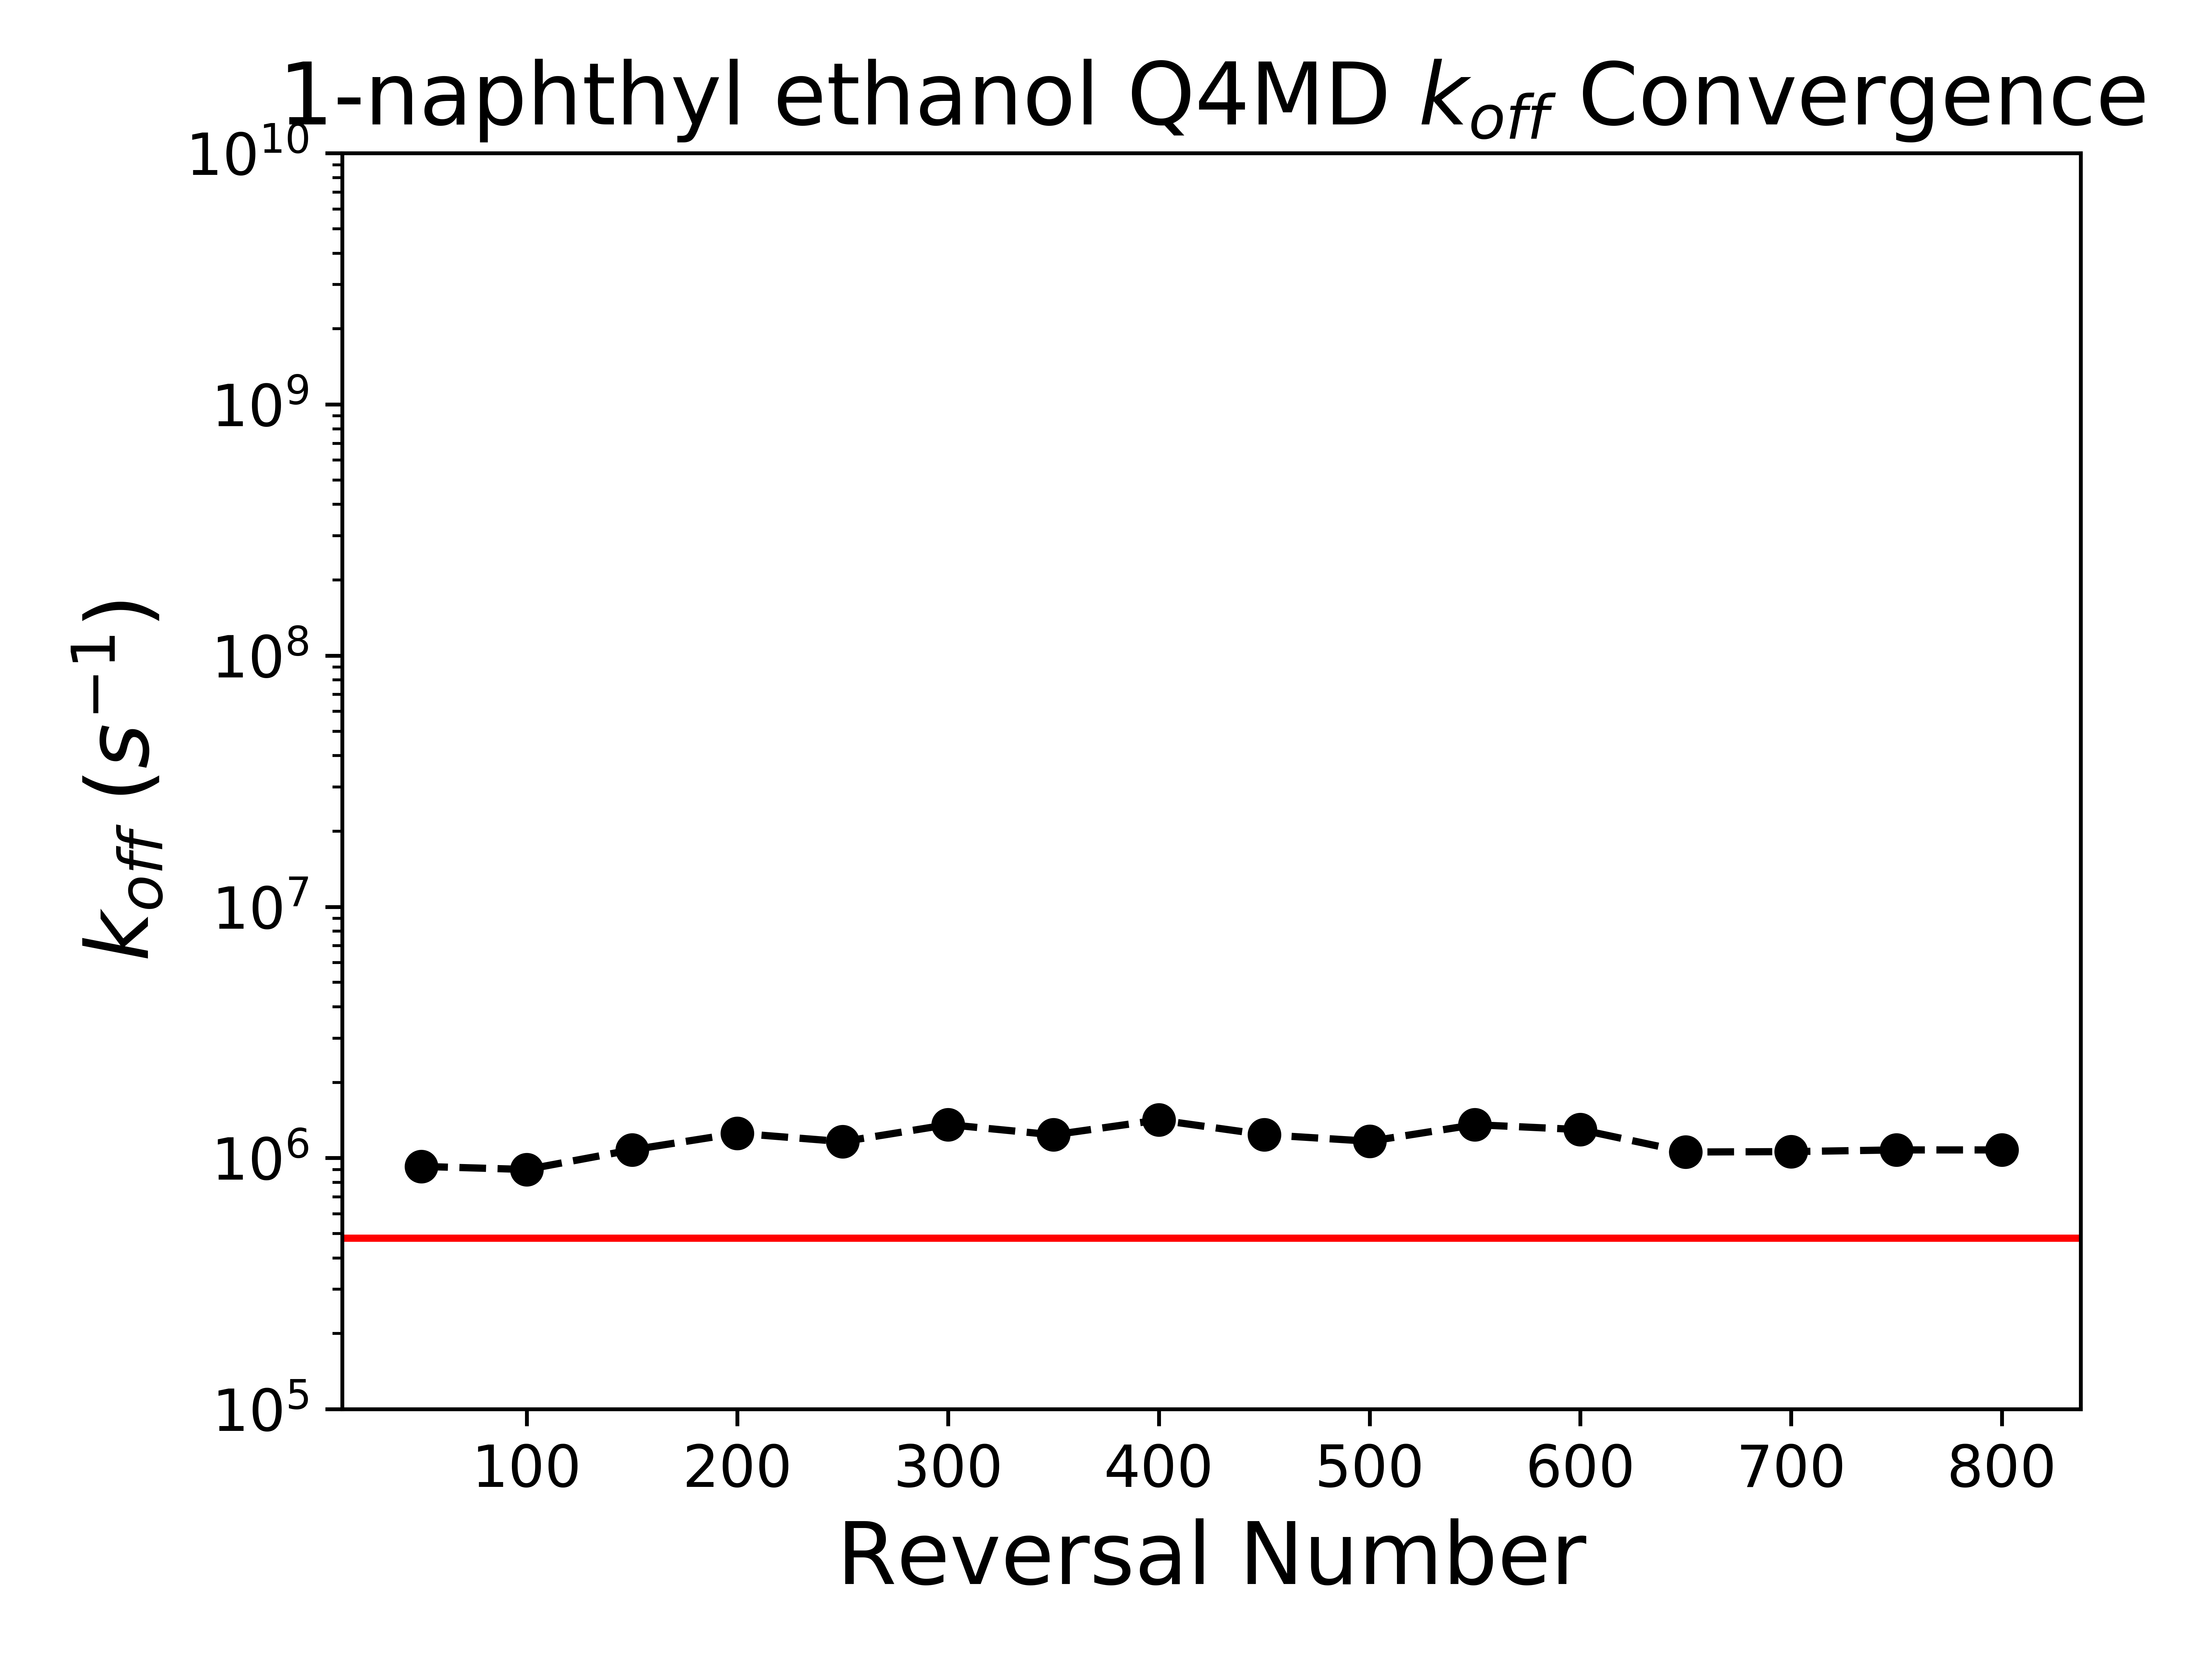
\includegraphics[width=\linewidth]{high_res_images/q4md_rate_conv_images/1-naphthylethanol_q4md_off_conv.png}
	\end{subfigure}
	\begin{subfigure}{0.3\linewidth}
		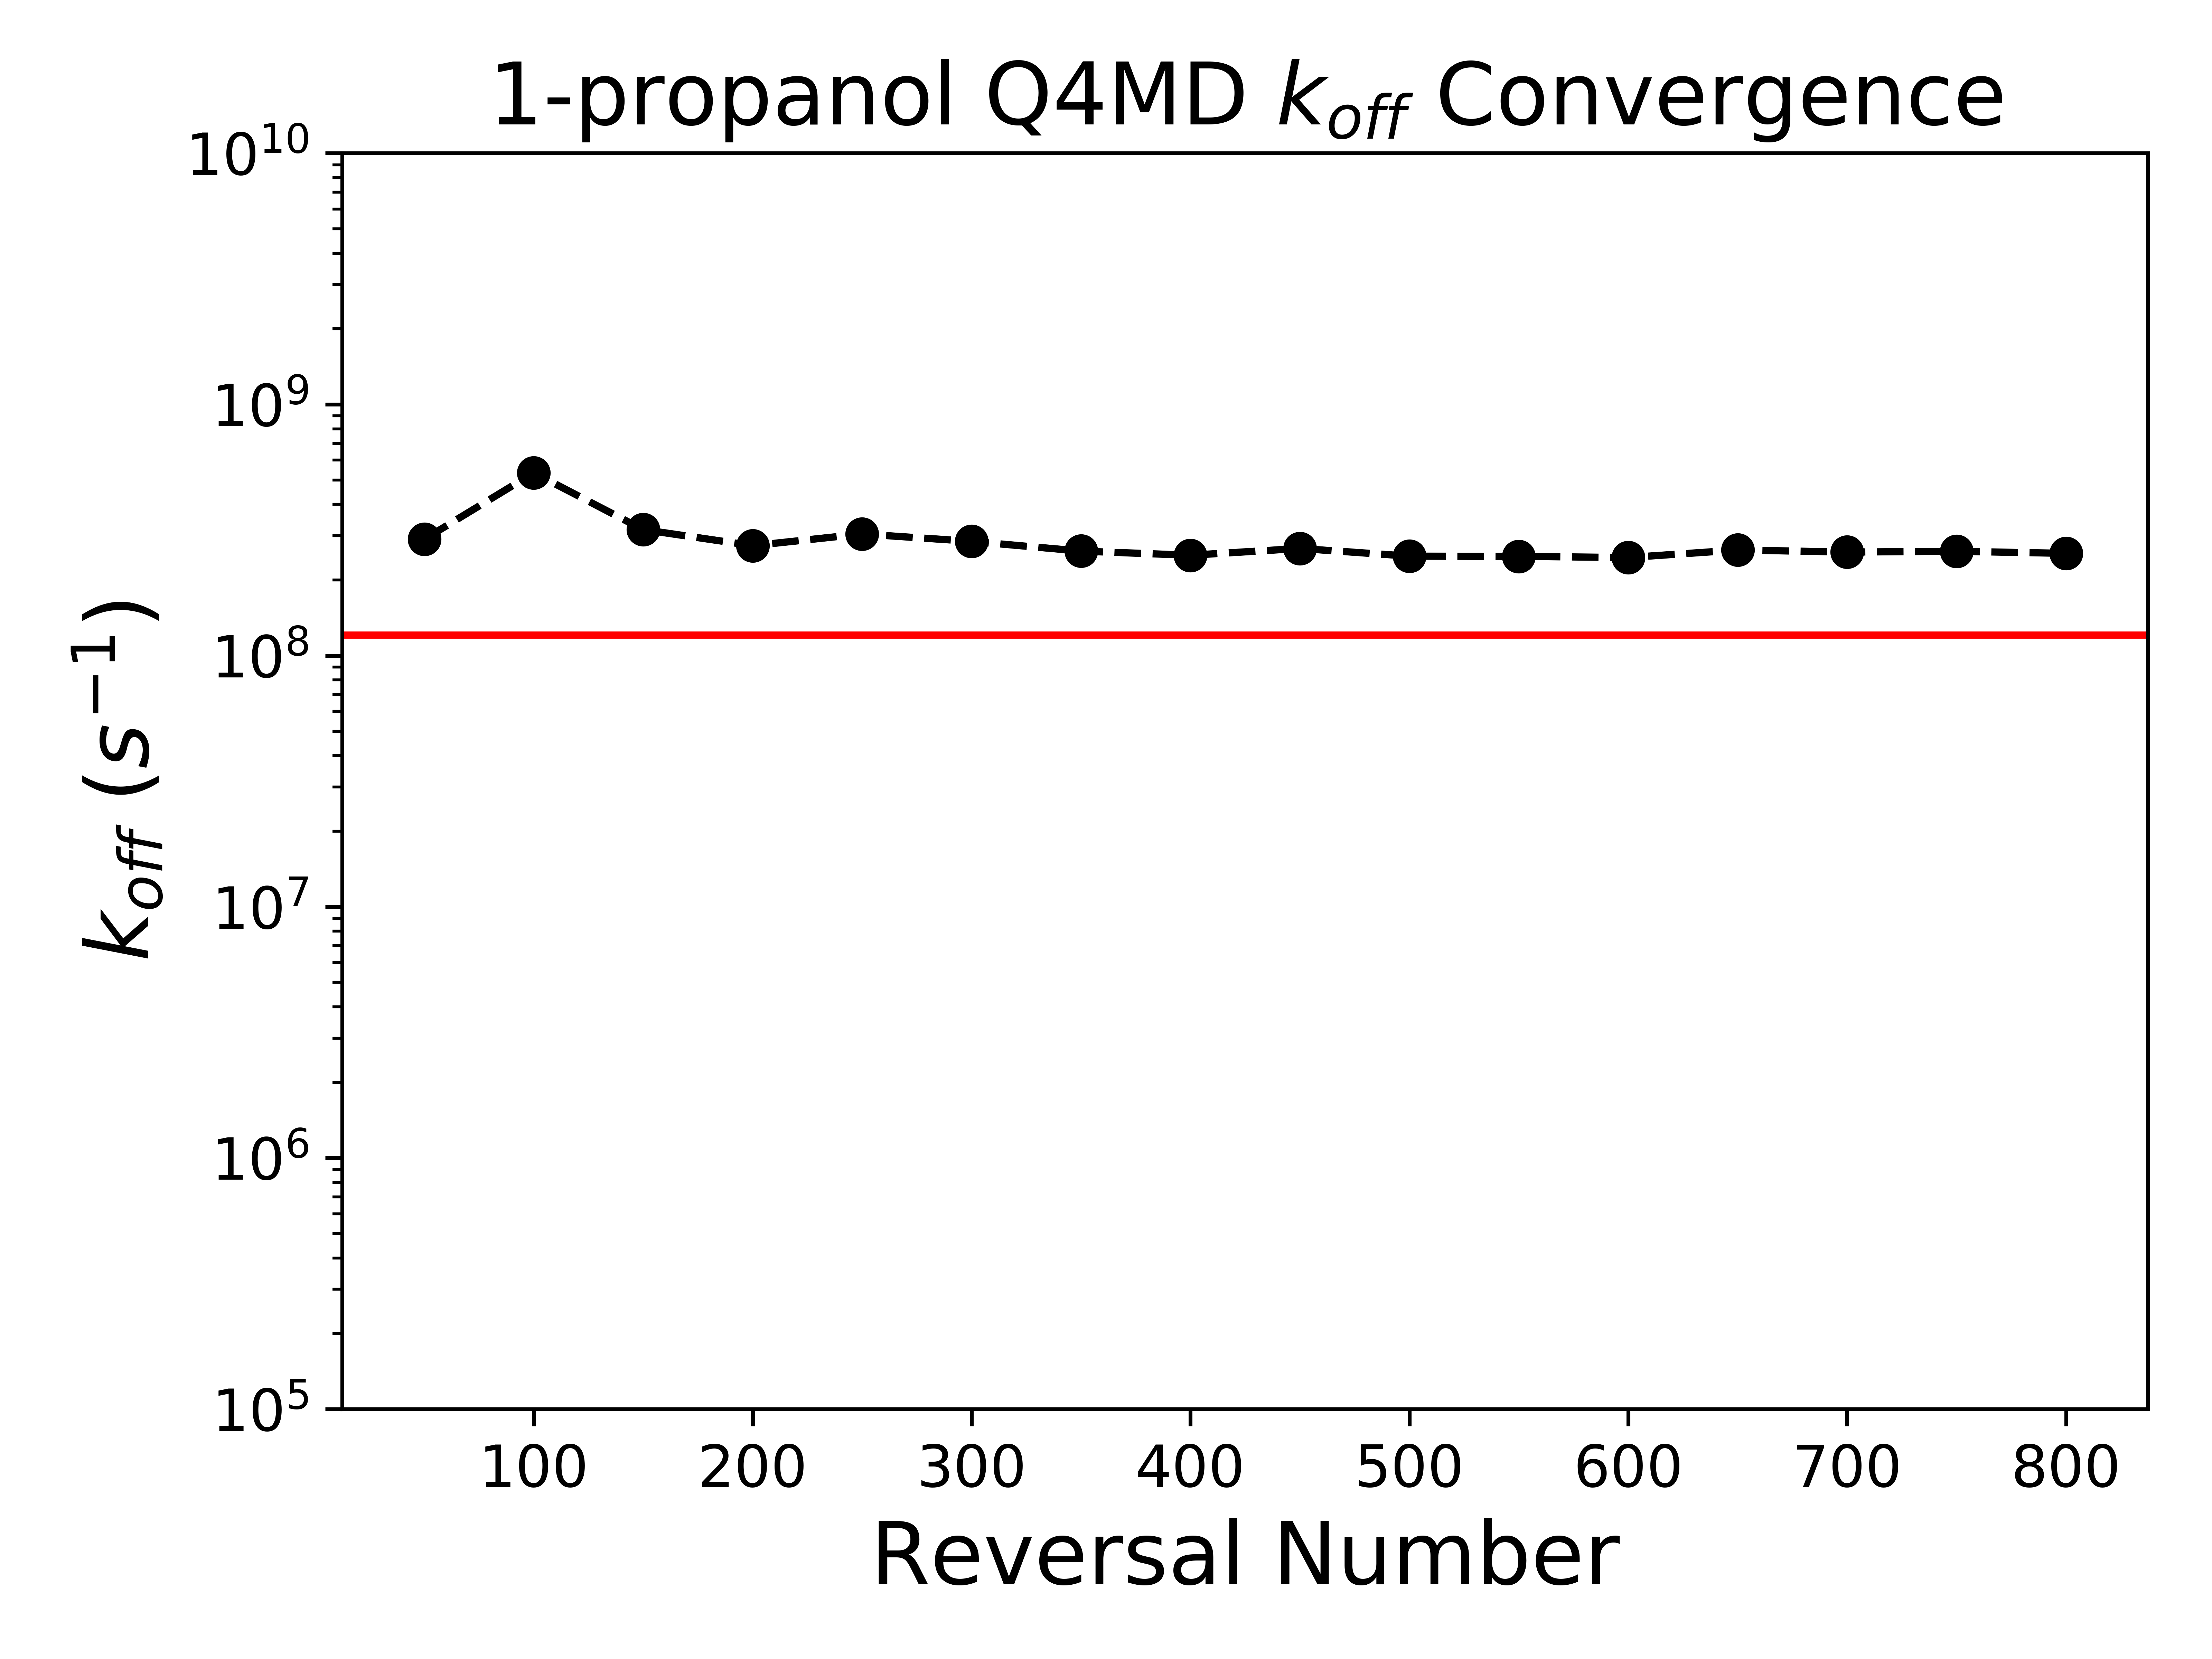
\includegraphics[width=\linewidth]{high_res_images/q4md_rate_conv_images/1-propanol_q4md_off_conv.png}
	\end{subfigure}
	\begin{subfigure}{0.3\linewidth}
		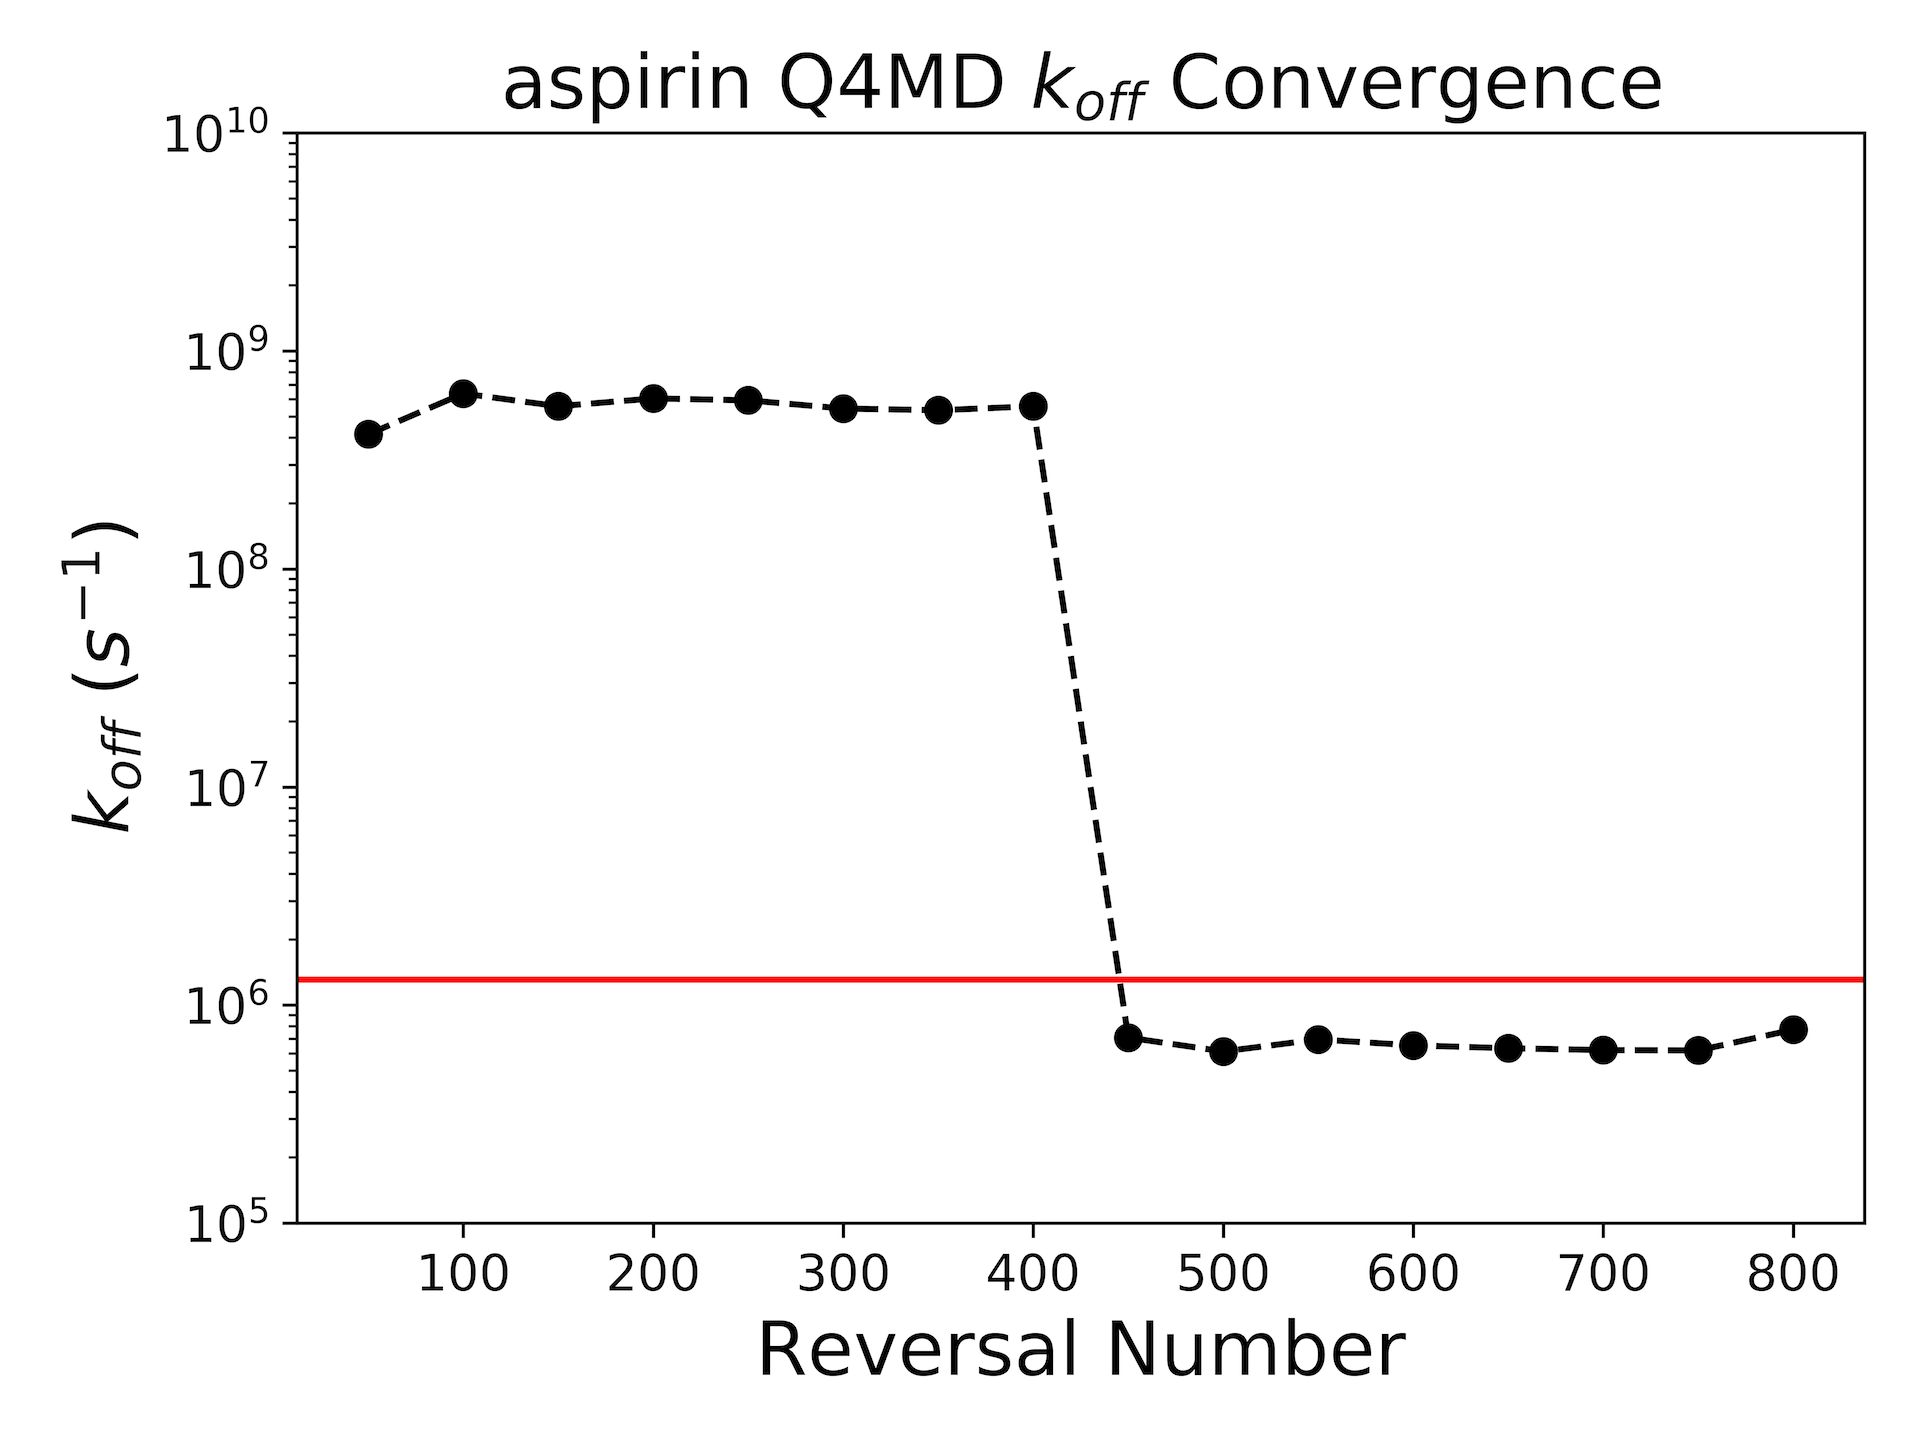
\includegraphics[width=\linewidth]{high_res_images/q4md_rate_conv_images/aspirin_q4md_off_conv.png}
	\end{subfigure}
	\caption{Convergence of off rates as a function of the number of reversals included using the Q4MD forcefield}
\end{figure}

\par Convergence of the rate constant is a highly complicated quantity dependent 
on the transition probabilities as well as the incubation times obtained from 
each milestone. Therefore, a more detailed analysis of the convergence of 
these quantities on a per milestone level can provide further insight into the 
overall convergence of a rate calculation within SEEKR. Fig.~\ref{fig:aspirin_conv_fig}a,b shows the convergence
of \kon and \koff, respectively, as a function of the number of reversals
launched for the representative system of Q4MD \bcd with aspirin. Reversal number is directly related to the length of
equilibrium sampling, the current bottleneck of a SEEKR
calculation.
While both values appear to converge in fewer than the maximum
number of reversals, the dramatic change in \koff after
reversal number 400 is of note. Further analysis of the
per-milestone transition counts (Fig.~\ref{fig:aspirin_conv_fig}c) and
incubation times (Fig.~\ref{fig:aspirin_conv_fig}d) revealed
that this change in \koff was due to poor initial sampling of
the -1.5 \AA milestone, which once sampled decreased the overall \koff. 

\begin{figure}
	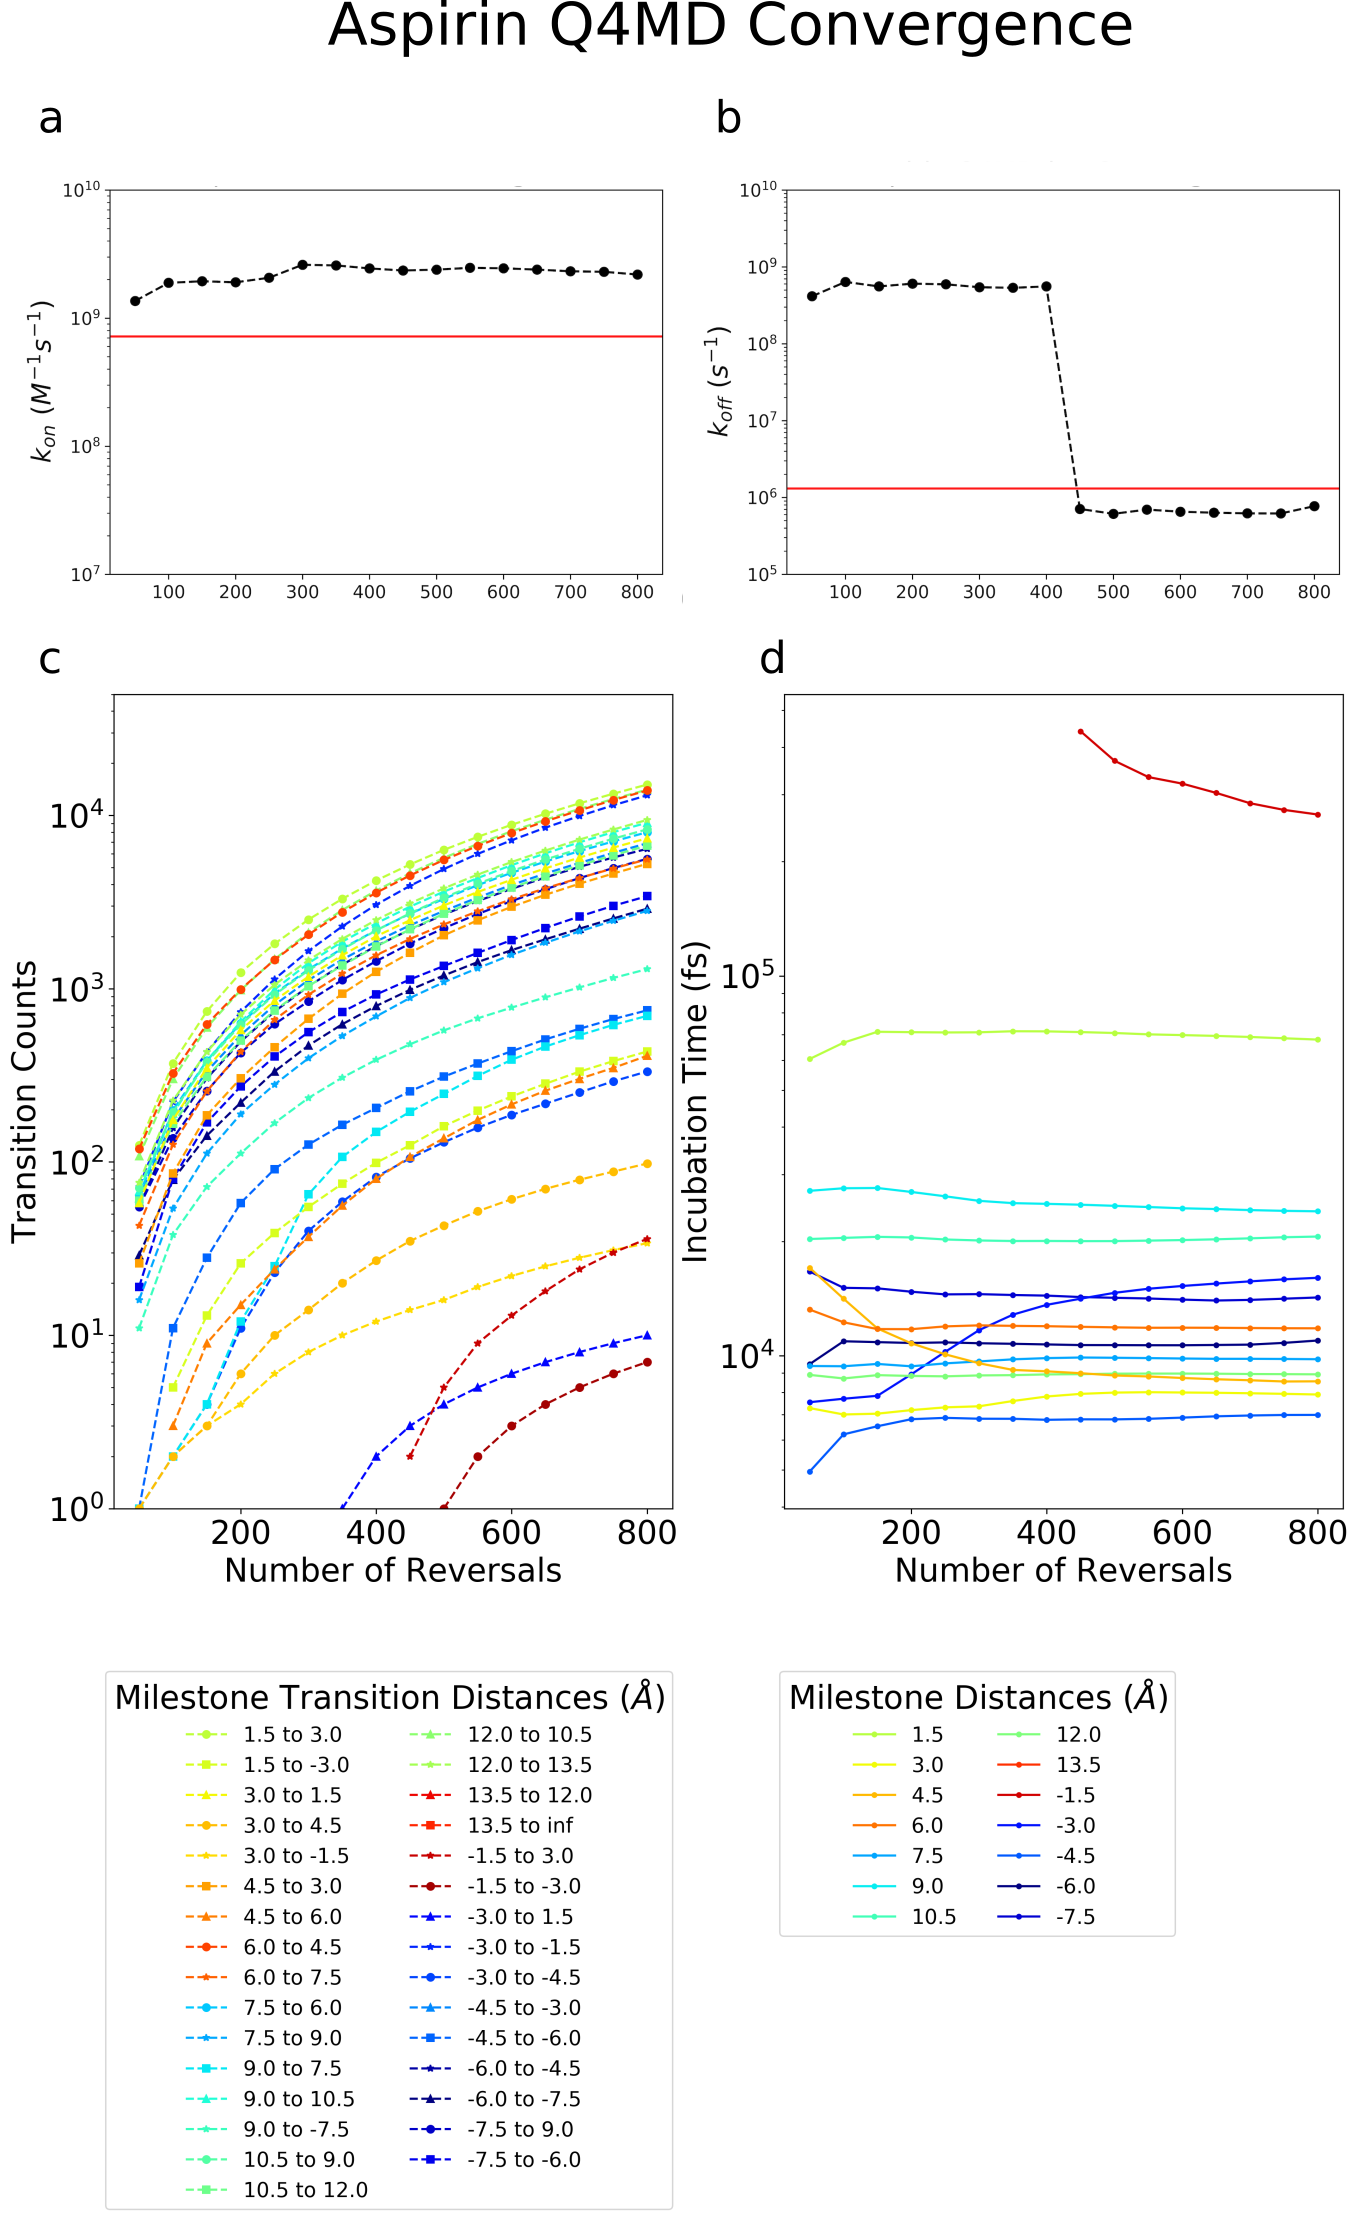
\includegraphics{images/aspirin_conv_comb.png}

	\caption{Convergence analysis for a representative ligand,  aspirin, and \bcd with the Q4MD forcefield. Convergence of a) \kon, b) \koff,  c) transition counts, and d) incubation times for each milestone are plotted as a function of the number of reversals launched.  Reversal number is directly related to the length of equilibrium sampling, as reversals were launched at 2 ns intervals from the equilibrium trajectory.}
	\label{fig:aspirin_conv_fig}
\end{figure}

This was only observed for the aspirin ligand, one of the bulkiest ligands, where it was extremely unlikely to observe transitions outward from the primary face due to steric effects. 
Evaluation of these convergence properties on a 
per milestone basis is a valuable diagnostic tool; identifying which 
milestones contribute most to the mean first passage time (and therefore \kon 
and \koff) and milestones where the ligand spends only a short time, providing 
detailed molecular insight into the binding and unbinding processes.
Furthermore, this analysis is also useful during the simulation process, 
as the convergence of each milestone can be assessed ``on the fly'' and individual simulations 
can be terminated or extended accordingly for each milestone.



%\subsubsection*{Milestoning Model}
\par We also explore the sensitivity of the calculated rate constants to the milestoning model construction. In particular, the appropriate 
spacing of milestones is critical for the calculation. Milestones must not be 
spaced so close such that the velocity of the system cannot decorrelate between 
transitions \cite{Vanden-Eijnden2008,West2007}. This assumption is typically 
valid for molecular dynamics simulations, as velocities typically decorrelate on 
the subpicosecond timescale \cite{Vanden-Eijnden2008}. However, if milestones are 
spaced far apart, transitions will require much longer simulations and 
milestioning sampling efficiency is lost.

For our systems, the incubation times of all milestones are on the order 
of multiple picoseconds or greater, which 
is longer than the sub-picosecond timescale typically necessary for decorrelation\cite{Vanden-Eijnden2008}.
When the milestone spacing was doubled to 3~\AA, simulation efficiency was 
dramatically reduced, such that few to no transitions between milestones were 
observed, precluding the calculation of rate constants. These observations suggest 
that the 1.5~\AA spacing used in our simulations was appropriate for the 
calculation of the desired kinetic parameters.

\par Our milestoning model differentiates the two faces 
of the cyclodextrin ring and therefore defines two bound states, corresponding 
to each face. Investigation into the effect of this on the resulting rate 
constants revealed that it had only minimal effects. When the two bound states 
were combined into a single milestone, only small changes to the rate were 
observed, within the error of both calculations. Furthermore, when the the two 
faces were not differentiated with unique milestones, minimal change in the 
calculated rate constants was observed. 

%\par We calculated the rates using both 
%milestoning models for the Q4MD system, where the calculated rate values are 
%smaller than the GAFF system and therefore changes in the value would be more 
%influential on the overall result.

%\par The calculated off rate values of all ligands were within the calculated 
%errors from both models. The only calculated on rate value that did not fall 
%within the error was aspirin, where the on rate increased from  
%$(2.19 \pm 0.12)\times 10^9$ $M^{-1}s^{-1}$ to $(2.90 \pm 0.14)\times 10^9$ $M^{-1}s^{-1}$.
%The minimal effect of these changes in the milestoning model on the calculated 
%rates is likely due to the extensive sampling achieved on both faces.

\par It is also important to note that our milestoning model did not explicitly 
resolve the ligand orientation in any way, and therefore any ligand orientational 
sampling was achieved entirely through simulation. This resulted in some ligand 
orientations being unsampled in the deepest milestones where the orientation was 
sterically restricted to the starting conformation on that milestone. While this 
is a limitation that will be addressed in future developments of SEEKR, it also 
highlights that a relatively simplistic model was able effectively calculate 
kinetic parameters with good agreement to experimental values.

\par The simplicity of this model has many advantages. The bound state is 
defined naturally as the innermost milestone and all other milestones can be 
defined at the same time, including what defines the unbound state. The long 
timescale MD employed a more empirical definition of the bound state where the 
ligand was only considered bound when the COM of the ligand was within 7.5~\AA 
of the COM of the $\beta$-cyclodextrin for at least 1.0~ns. Similarly the ligand 
was considered unbound when it left this 7.5~\AA bound state for at least 1.0~ns.
With the SEEKR approach, minimal prior knowledge of the system is required, as 
binding and unbinding are determined only from the milestone surfaces. No time 
cutoff is required, as short excursions that do not result in full binding and 
unbinding events are captured naturally in the milestoning model. The simplicity of SEEKR milestoning calculation setup, in conjunction with
the ability to monitor convergence for each milestone and terminate
simulations accordingly, makes this approach well-suited for
calculations with multiple ligands as would be necessary in a drug
discovery setting.

% Conclusions  (JC?)
%  *difficulties that arise in the calculations - slow membrane reorganization, solute reorientation, etc.  (here and/or maybe intro?)
%  *what method to use, when, how to prepare?
%  *where best to invest limited computational time? 
%  *how much sampling is really needed to get within a certain error?  (e.g., +/- 1 log unit)
%  *take home message: can MD ever be used to reliably predict permeabilities?  
%   -is there a way to streamline the process for high throughput calculations?
%

\section*{Conclusions}

We have computed the membrane permeability to three compounds using a variety of simulation-based methods, namely US and ABF, along with their multiple-copy variants, REUS and MW-ABF, respectively.  These three compounds, codeine, benzoic acid, and urea, span a range of chemical properties and, most importantly, permeabilities (see Table~\ref{table:results}).  All simulation methods were able to predict the permeability within one log unit typically, except in a few cases that were off by 1.5 (see Fig.~\ref{fig:deltaP}).  Interestingly, of the four methods tested, none stood out as unequivocally better than the others.  The root-mean-square error in log units for each method was 0.821 (US), 1.23 (REUS), 1.33 (ABF), and 1.08 (MW-ABF). 

Because of their similar performances, no one simulation method is recommended over another.  However, regardless of the method chosen, certain procedures can improve convergence.   It was found that simulation over the entire range, i.e., from one side of the membrane to the other, followed by symmetrization of the resulting PMF converged much faster than simulating over just half the range, i.e., from one side to the membrane center (see Fig.~S5).  Additionally, the states used to seed the windows for production sampling should be well equilibrated.  Methods such as SMD used to produce these initial states induce significant non-equilibrium perturbations to the membrane that may take hundreds of nanoseconds or more to equilibrate.  Alternatives to SMD include building the membrane {\it de novo} around the permeant at varying depths~\cite{Dorairaj2007} or introducing the permeant in a perturbative fashion at different values of $z$.  Regardless of the method, equilibration should be carried out for as long as is feasible (50-100\,ns/window at least, depending on membrane depth), particularly when the permeant's stability relies upon the spontaneous formation of membrane defects and penetration of water.

Two methods for calculating the diffusivity were explored.  The first, more commonly used Generalized Langevin method, based on restraining the solute and measuring the correlation of the system forces acting on it, was combined with the PMFs in the US and REUS; the second, the Bayesian inference method, was combined with PMFs from ABF and MW-ABF.  Both methods present a number of subtleties that prevent a straightforward calculation of $D$($z$), e.g., a proper choice of the force constant in the Generalized Langevin method or the discretization time step in Bayesian inference.  Furthermore, they are both plagued by long correlation times that are not amenable to the usual MD time scales.  Despite these caveats, they produced diffusivity profiles in rough agreement, although those from the Bayesian inference method are consistently slightly higher in the membrane than those from the Generalized Langevin method (see Fig.~\ref{fig:Dz}).  

Because the solubility-diffusion model relies on two position-dependent quantities, the PMF and the diffusivity, it is natural to assume they must be calculated to determine the permeability.  However, as demonstrated in the section ``Comparison of methods and tolerance to error'', only a few data points contribute significantly to it.  Therefore, permeability can be estimated from a handful of parameters, namely the values of $W$($z$) and $D$($z$) at the membrane/water interface and at the membrane center, with the remainder interpolated from an expected smooth topology.  Going even further, extrapolating from just a single value each of the PMF and the diffusivity at the membrane center for urea (see Fig.~\ref{fig:models}A) produced a log\perm~almost identical to the experimental value.  Thus, we recommend that sampling be focused on critical regions where barriers are expected, e.g., the membrane core and/or interfacial region.

Taken together, the results show the robustness of a variety of MD-based methods in calculating membrane permeability for small molecules.  In particular, all methods {\color{red} appear to} converge on sub-$\mu$s time scales, although the determined log\perm~values are nearly all 0.5 to 1.5 log units above the experimental values.  This consistent overestimation is in agreement with a previous MD study from 2004~\cite{Bemporad2004}, despite using 10-100$\times$ longer simulations in the current study.  {\color{red} The membranes compared, DMPC in simulation with egg PC in experiment, are not identical, which may contribute to the discrepancy.}  Another possible reason could be slow membrane reorganization that occurs on a time scale even an additional 2-3 orders of magnitude greater~\cite{Neale2011}.  The lack of polarizability is another tempting possibility, given the vastly different environments experienced by the permeating molecule~\cite{Riahi2014}.  
Similarly, the most commonly used force fields (including CGenFF used in this study) are primarily parameterized to reproduce phenomena obtained in aqueous environments. Thus, it may be unrealistic to expect that solute phenomena within the non-polar membrane environment is as well represented. Therefore, further exploration of the force-field effects within lipid-like or non-polar environments are warranted.  In particular, inclusion of explicit polarizability may improve accuracy, although at a computational cost of 2-6$\times$~\cite{Chowdhary2013,Wang2013}.  {\color{red} However, given the lack of convergence of the four methods to a single value for each permeant, all of which use the same force field, it cannot be known a priori to what degree, if any, changes to the force field will improve agreement with experiment.}
Additionally, the assumptions of the solubility-diffusion model, such as the reliance on a single reaction coordinate and that permeation obeys classical diffusion, may need to be challenged to obtain improved quantitative agreement with experimental measures~\cite{Orsi2010,Parisio2013,Comer2014}.

Finally, we draw attention to the potential benefit of our results to QSPR models.   
%Even if the explicit-membrane permeability calculations reported here were perfectly accurate, they are still too computationally demanding to replace QSPR, taking weeks where results are needed in less than a day.  However, 
We have shown that only one or two points in the PMF and diffusivity contribute significantly to the permeability.  Thus, calculations for a single permeant focusing on these critical points could be done in hours on a sufficiently fast cluster.  Furthermore, the location of these points, typically at the membrane center or at the water/membrane interface, suggest reduced systems that could represent them reasonably well, e.g., octanol for the interfacial region.  
Combined with improved force fields, fast calculations on such reduced systems could augment the molecular descriptors used to design QSPR models, similar to the ``membrane-interaction QSAR'' approach pioneered by Hopfinger et al.~\cite{Kulkarni1999,Tseng2012}.





%!TEX root = BCD.tex

\section*{Computational Methods}

\par GAFF\cite{Wang2004,Wang2006} forcefield parameters for the seven guest molecule
along with both GAFF and Q4MD-CD\cite{Cezard2011} parameterizations of $\beta$-cyclodextrin 
were obtained from Tang and Chang\cite{Tang2017}. For comparison we use identical structures and
parameterizations as those used in their study. These initial structures were 
used by the SEEKR software for preparation of the milestoning simulations. 
The preparation procedure was the same for each of the seven guest molecules and 
followed standard SEEKR protocols\cite{Votapka2017}. All systems were solvated 
with TIP3P waters\cite{Jorgensen1983a}. All BD simulations were performed using the BrownDye software package\cite{Huber2010}. 
Electrostatic potentials of the host and guest molecules used as inputs for the 
BD simulation were calculated with APBS version 1.4\cite{Baker2001}. 
A modified version of NAMD 2.12 was used for all MD simulations\cite{Phillips2005}.
For all 13 milestones in the MD region, the standard SEEKR procedure for 
minimization, equilibration and simulation was followed. In total, 2.6~${\mu}s$ of equilibrium sampling (160~ns for 16 milestones) were 
used and approximately 570~ns of FHPD sampling for a total of 3.2~${\mu}s$ of 
simulation used in the milestoning model. The total cost per ligand (including 
simulation discarded for equilibration) was therefore $\sim$3.8 ${\mu}s$. 
\section*{Supporting Information}

The following is made available online:
Additional computational details, calculated rate values, 
convergence plots for all ligands

\section*{Acknowledgements}
We thank Zhiye Tang and Chia-en Chang for sharing structures and parameters as 
well as helpful discussions. This work is funded in part by the Director's 
New Innovator Award Program NIH DP2-OD007237, the National Biomedical Computation
Resource (NBCR) NIH P41-GM103426, and the National Science Foundation through 
XSEDE supercomputing resources provided via TG-CHE060073 to R.E.A. B.R.J. 
and C.T.L. also acknowledge support from the NIH Molecular Biophysics 
Training Program (T32-GM008326).

\bibliography{libraryU.bib,journals_short.bib}

\end{document}  
